\documentclass[12pt,a4paper]{article}
\usepackage[utf8]{inputenc}
\usepackage{amsmath}
\usepackage{amsfonts}
\usepackage{amssymb}
\usepackage{graphicx}
\usepackage{subcaption}
\usepackage{float}

\author{Team Gamma \\ {\small Ajda Frankovič, Martin Preradović, Niki Bizjak}}
\title{Colour recognition}
\date{}
\begin{document}
	
	\maketitle
	
	For our second task we were training a classifier to recognize six different colours - red, green, blue, yellow, white and black. We divided the task into three parts. 

	\begin{enumerate}
		\item Obtaining data for training and testing set
		\item Training different classifiers
		\item Evaluating the performance of trained classifiers
	\end{enumerate}
		
	\section{Preparing training and testing data}

	The first, most time consuming part was obtaining training and testing sets - images of unicolor objects under different conditions (illumination and viewing angle). After the training and testing data sets were created, each image had to be labelled and cropped so it only contained the object of interest. \\

	\subsection{Taking photos}
	
	We chose to take two groups of photos. For the first set of images we took photos of unicolor circles under different viewing angles and under different light conditions. We played with not just the light intensity but also it's colour as can be seen in the photos below. We obtained around 200 images of this kind. For simplicity, we used a simple unicolor circles of different colours. The circular shape was selected because it is easy to detect and cropping can be done automatically using Hough transformation method. \\
	
	Below we present a subset of our training and testing images below. It can be seen that some of the pictures were taken in dark environment, some were taken under blue / yellow lights, we also tried using very high ISO to simulate grain, etc. We also included multiple different shades of the same colour. This is important because the color of 3D objects that our robot will encounter won't be of an uniform colour. Some parts of the objects will be darker, some lighter and the overall shade will change depending on which direction the robot will see the object from.

	\begin{figure}[H]
		\centering
		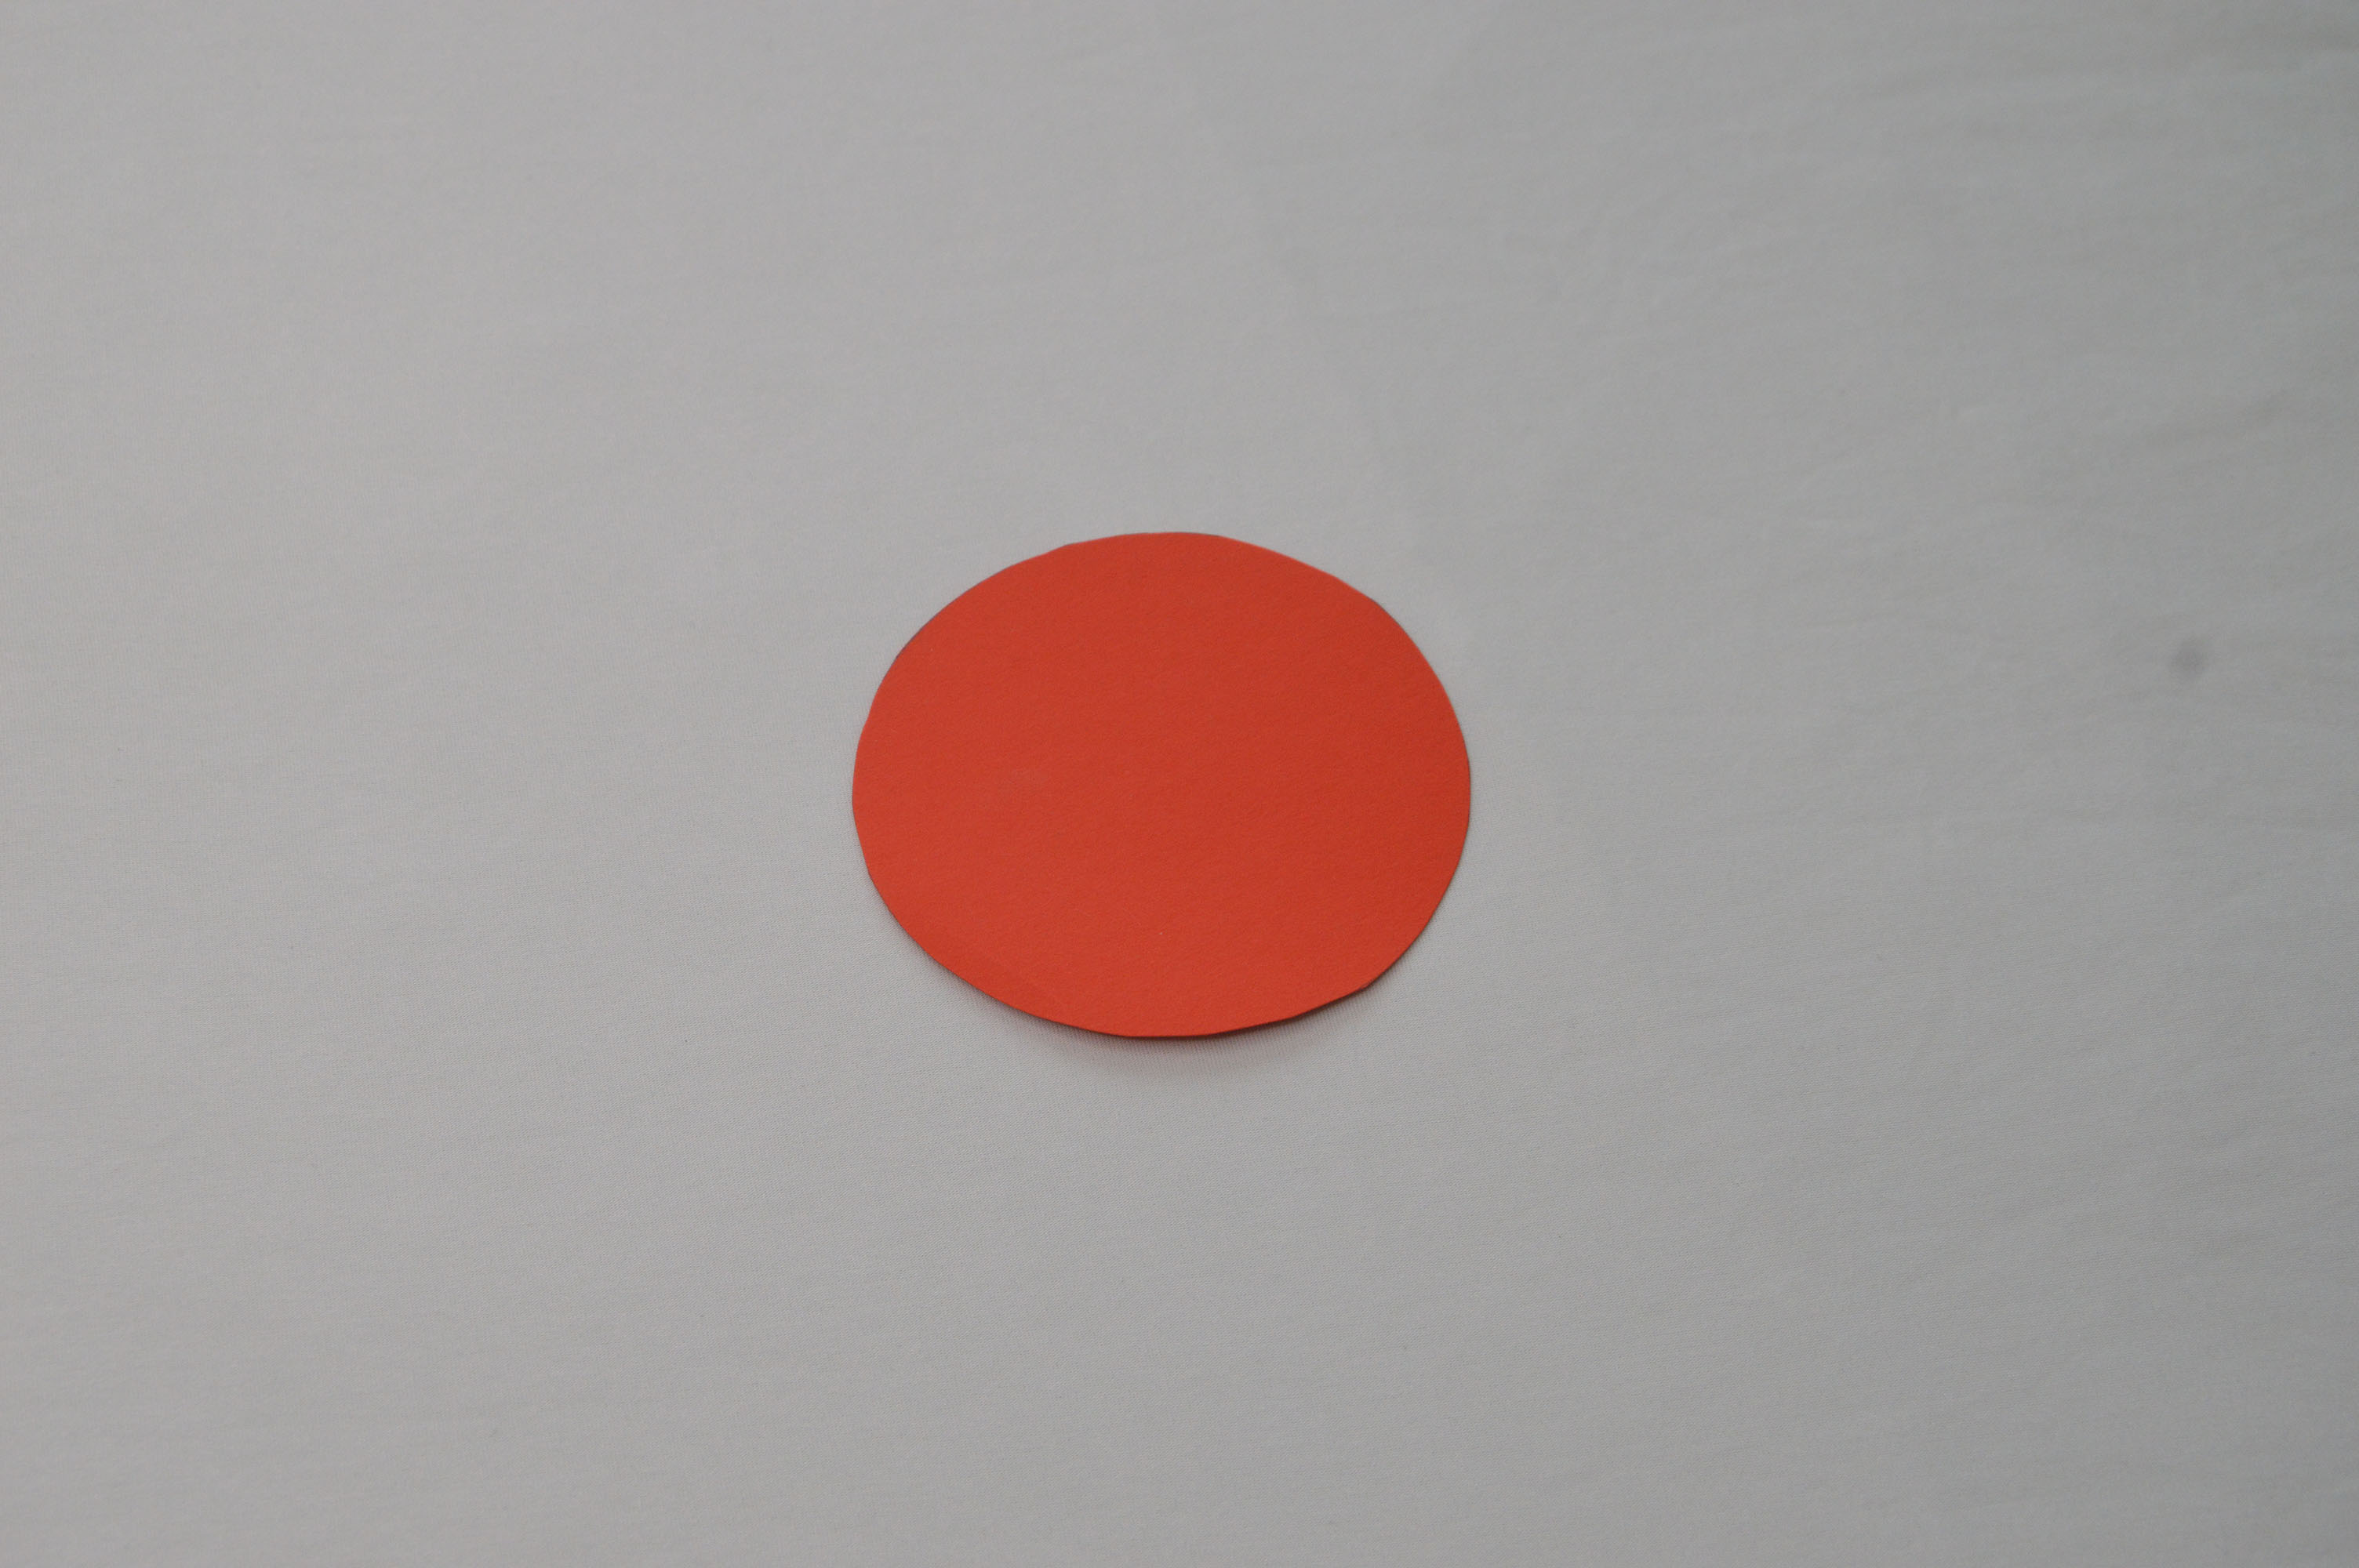
\includegraphics[width=.20\linewidth]{images/train01.jpg}
		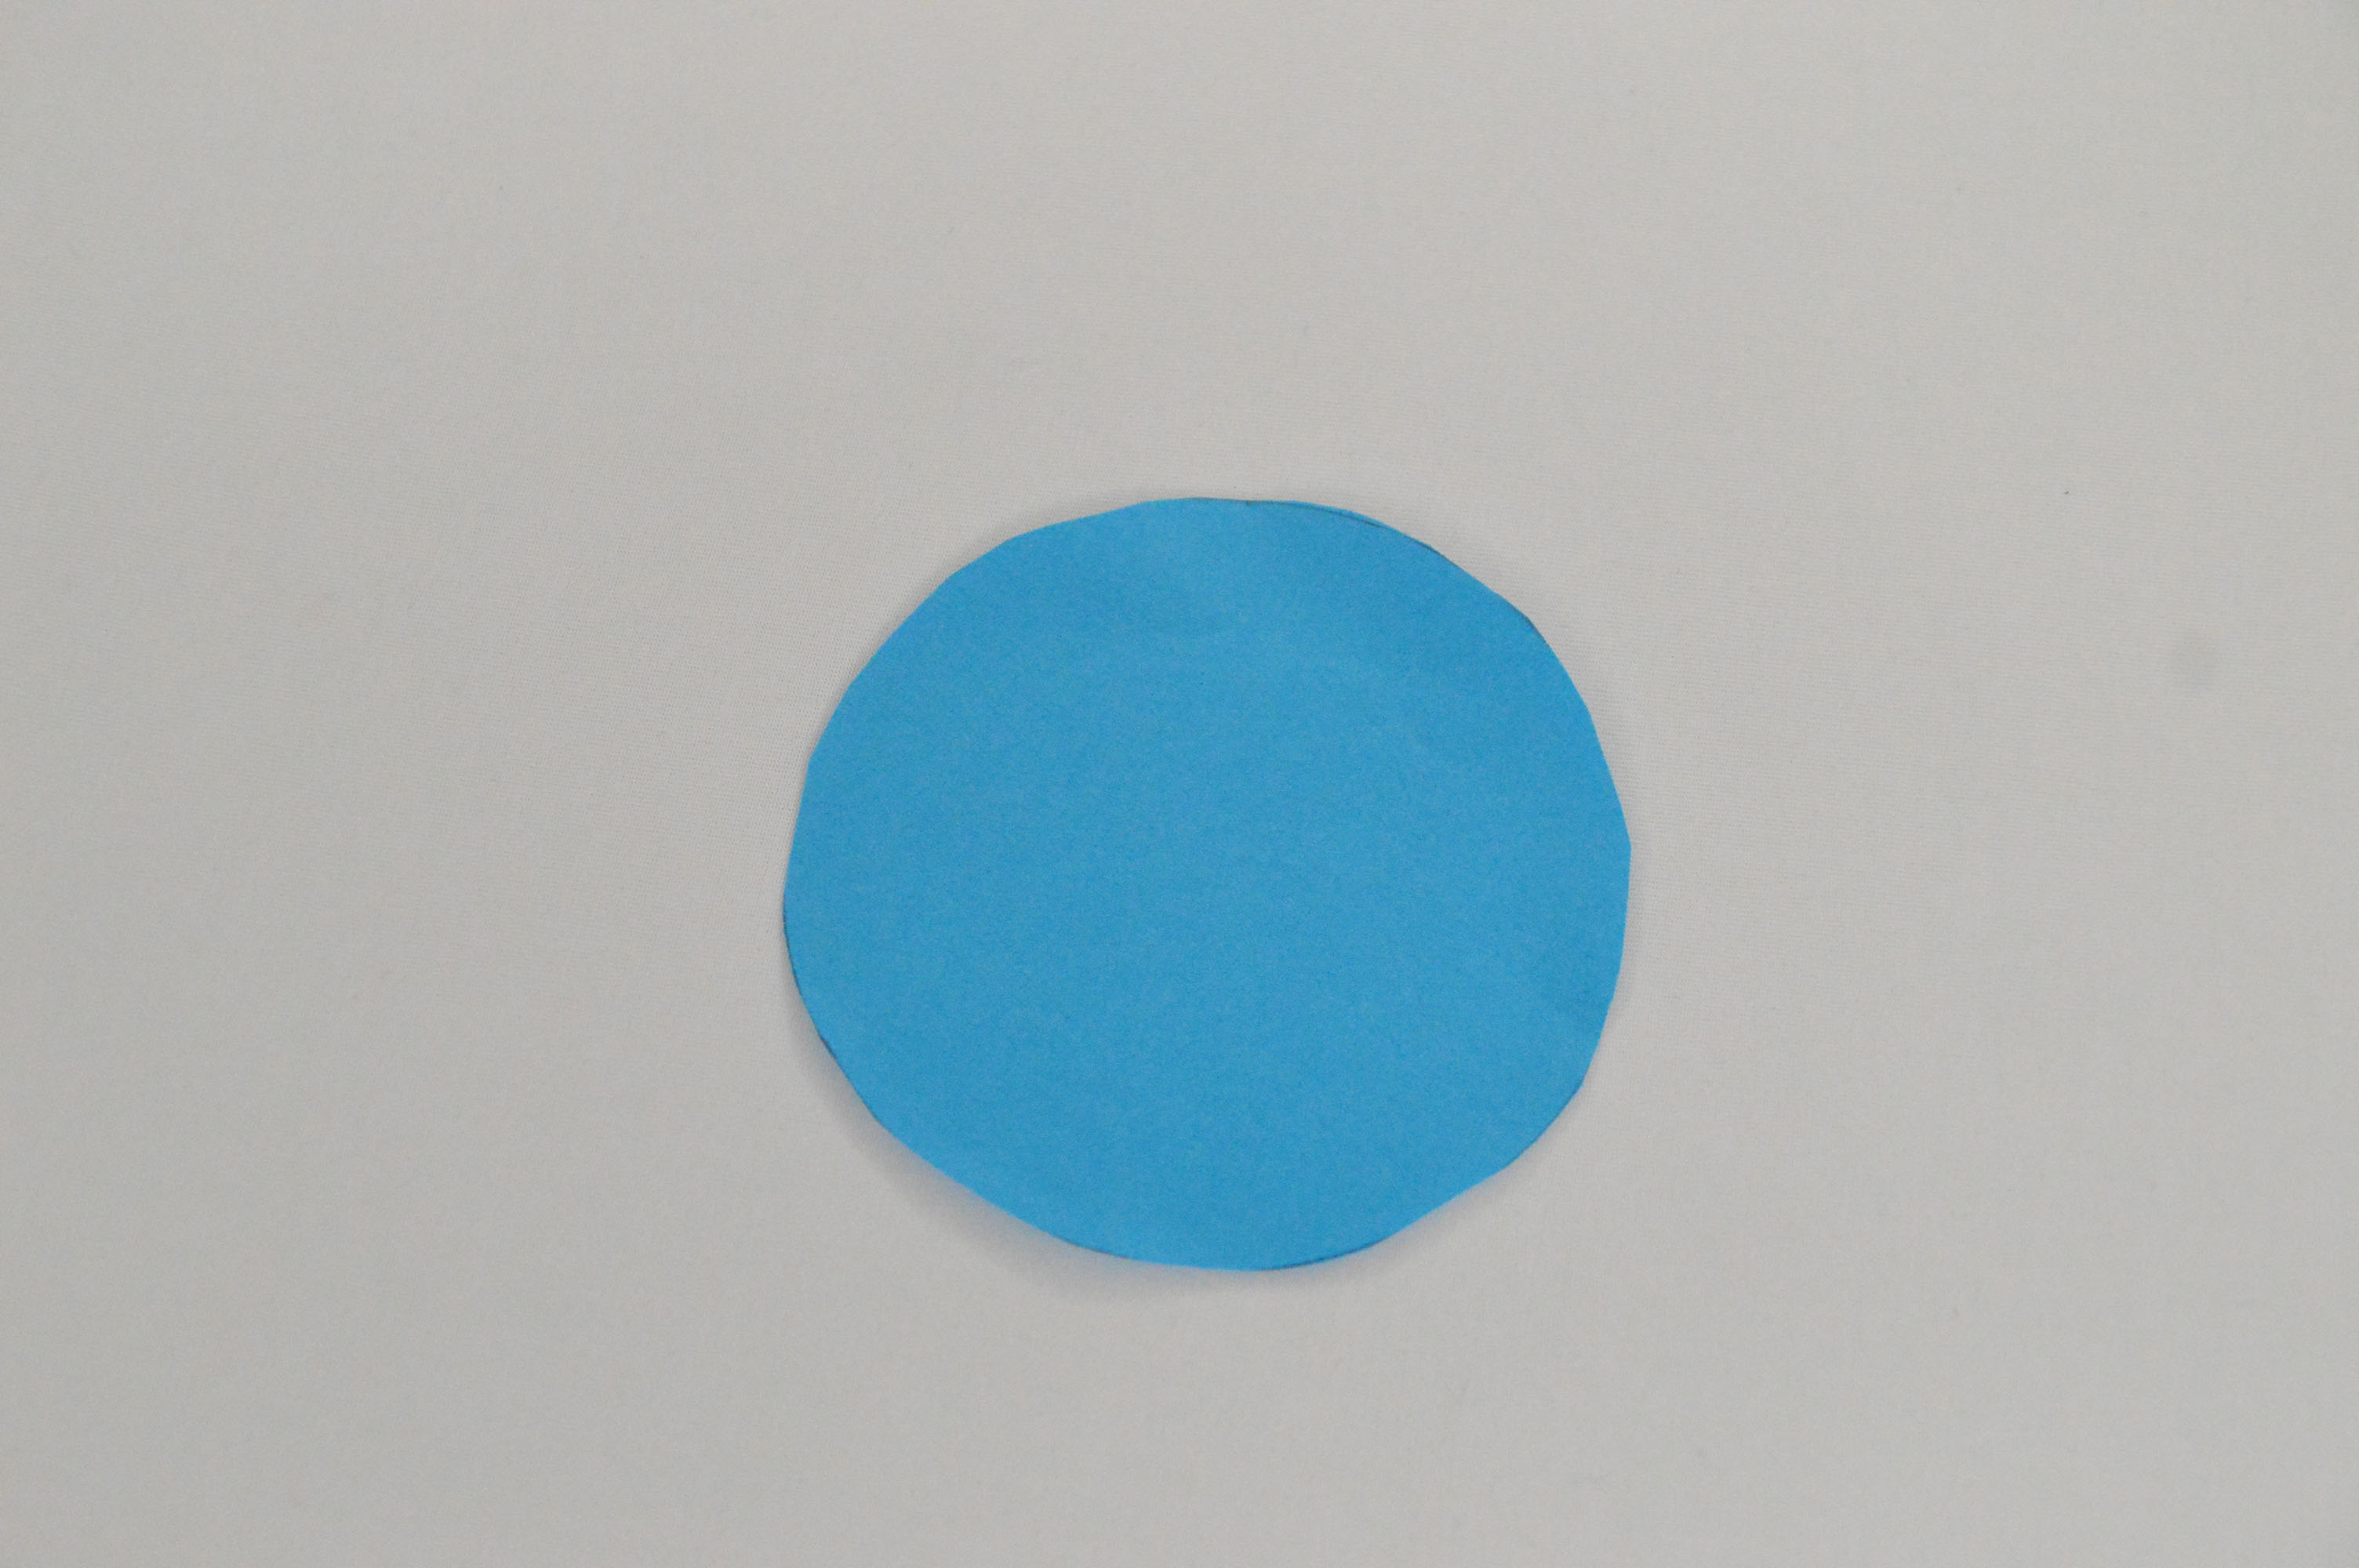
\includegraphics[width=.20\linewidth]{images/train02.jpg}
		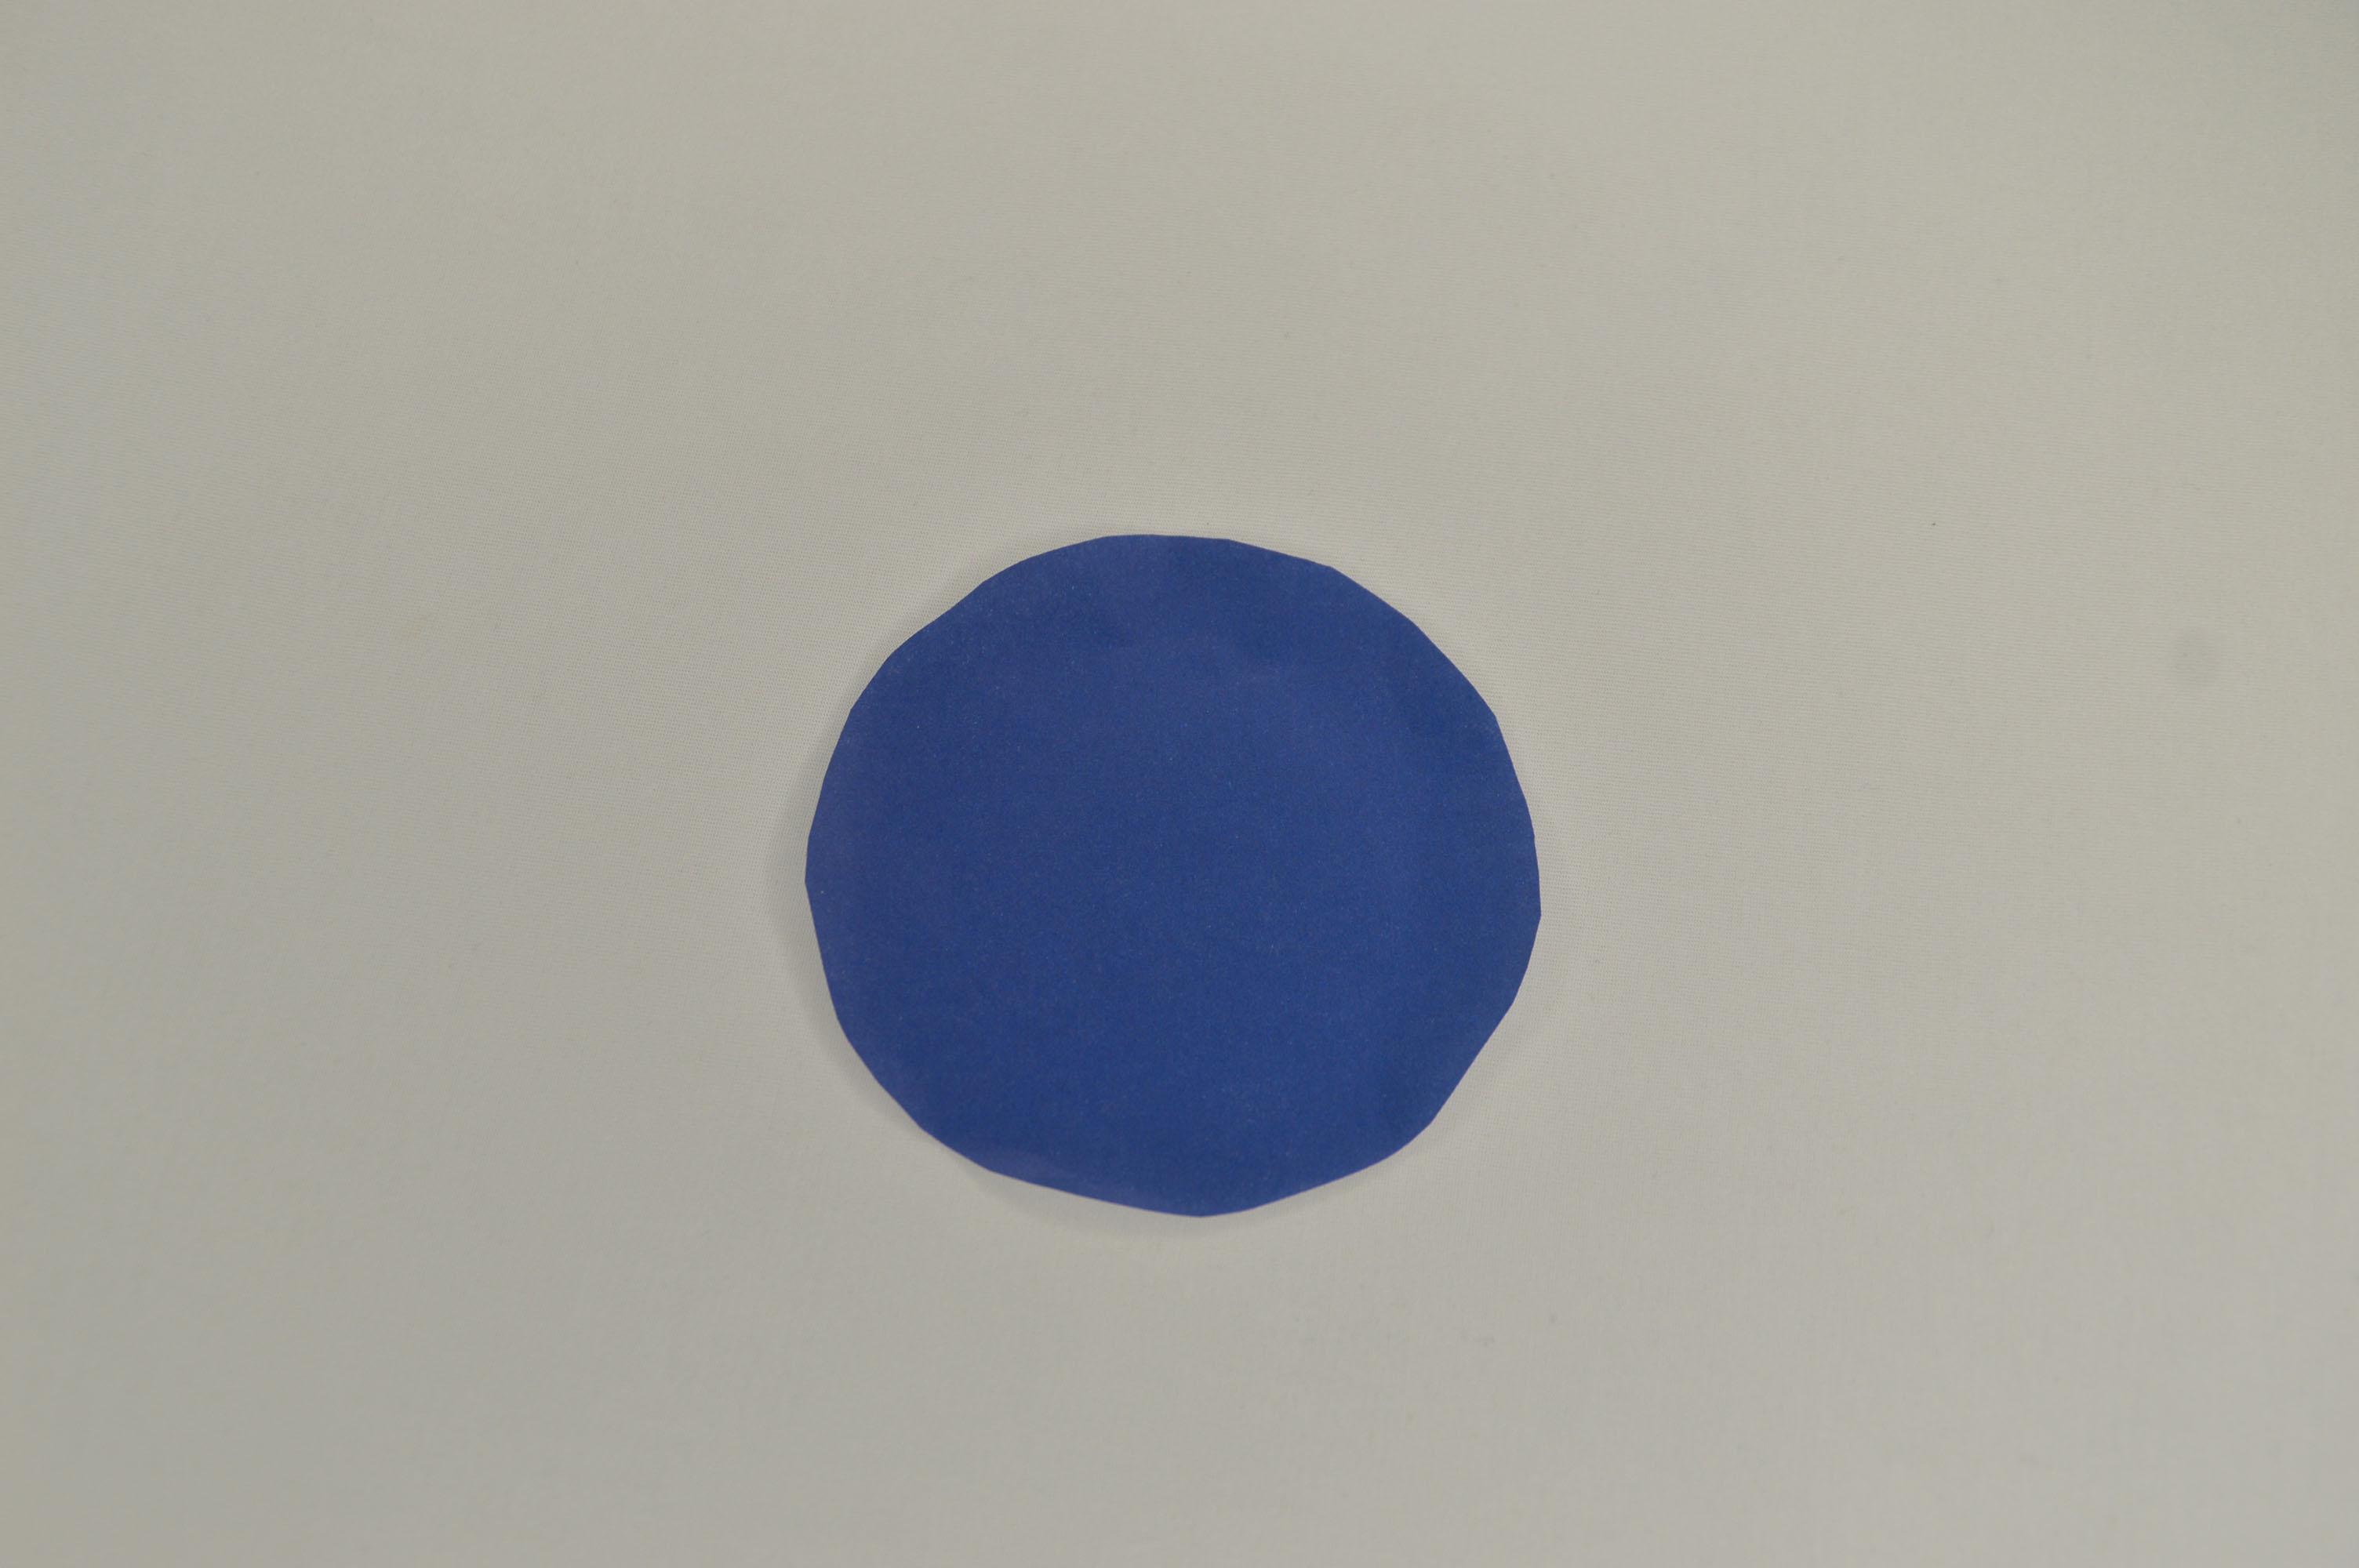
\includegraphics[width=.20\linewidth]{images/train03.jpg}
		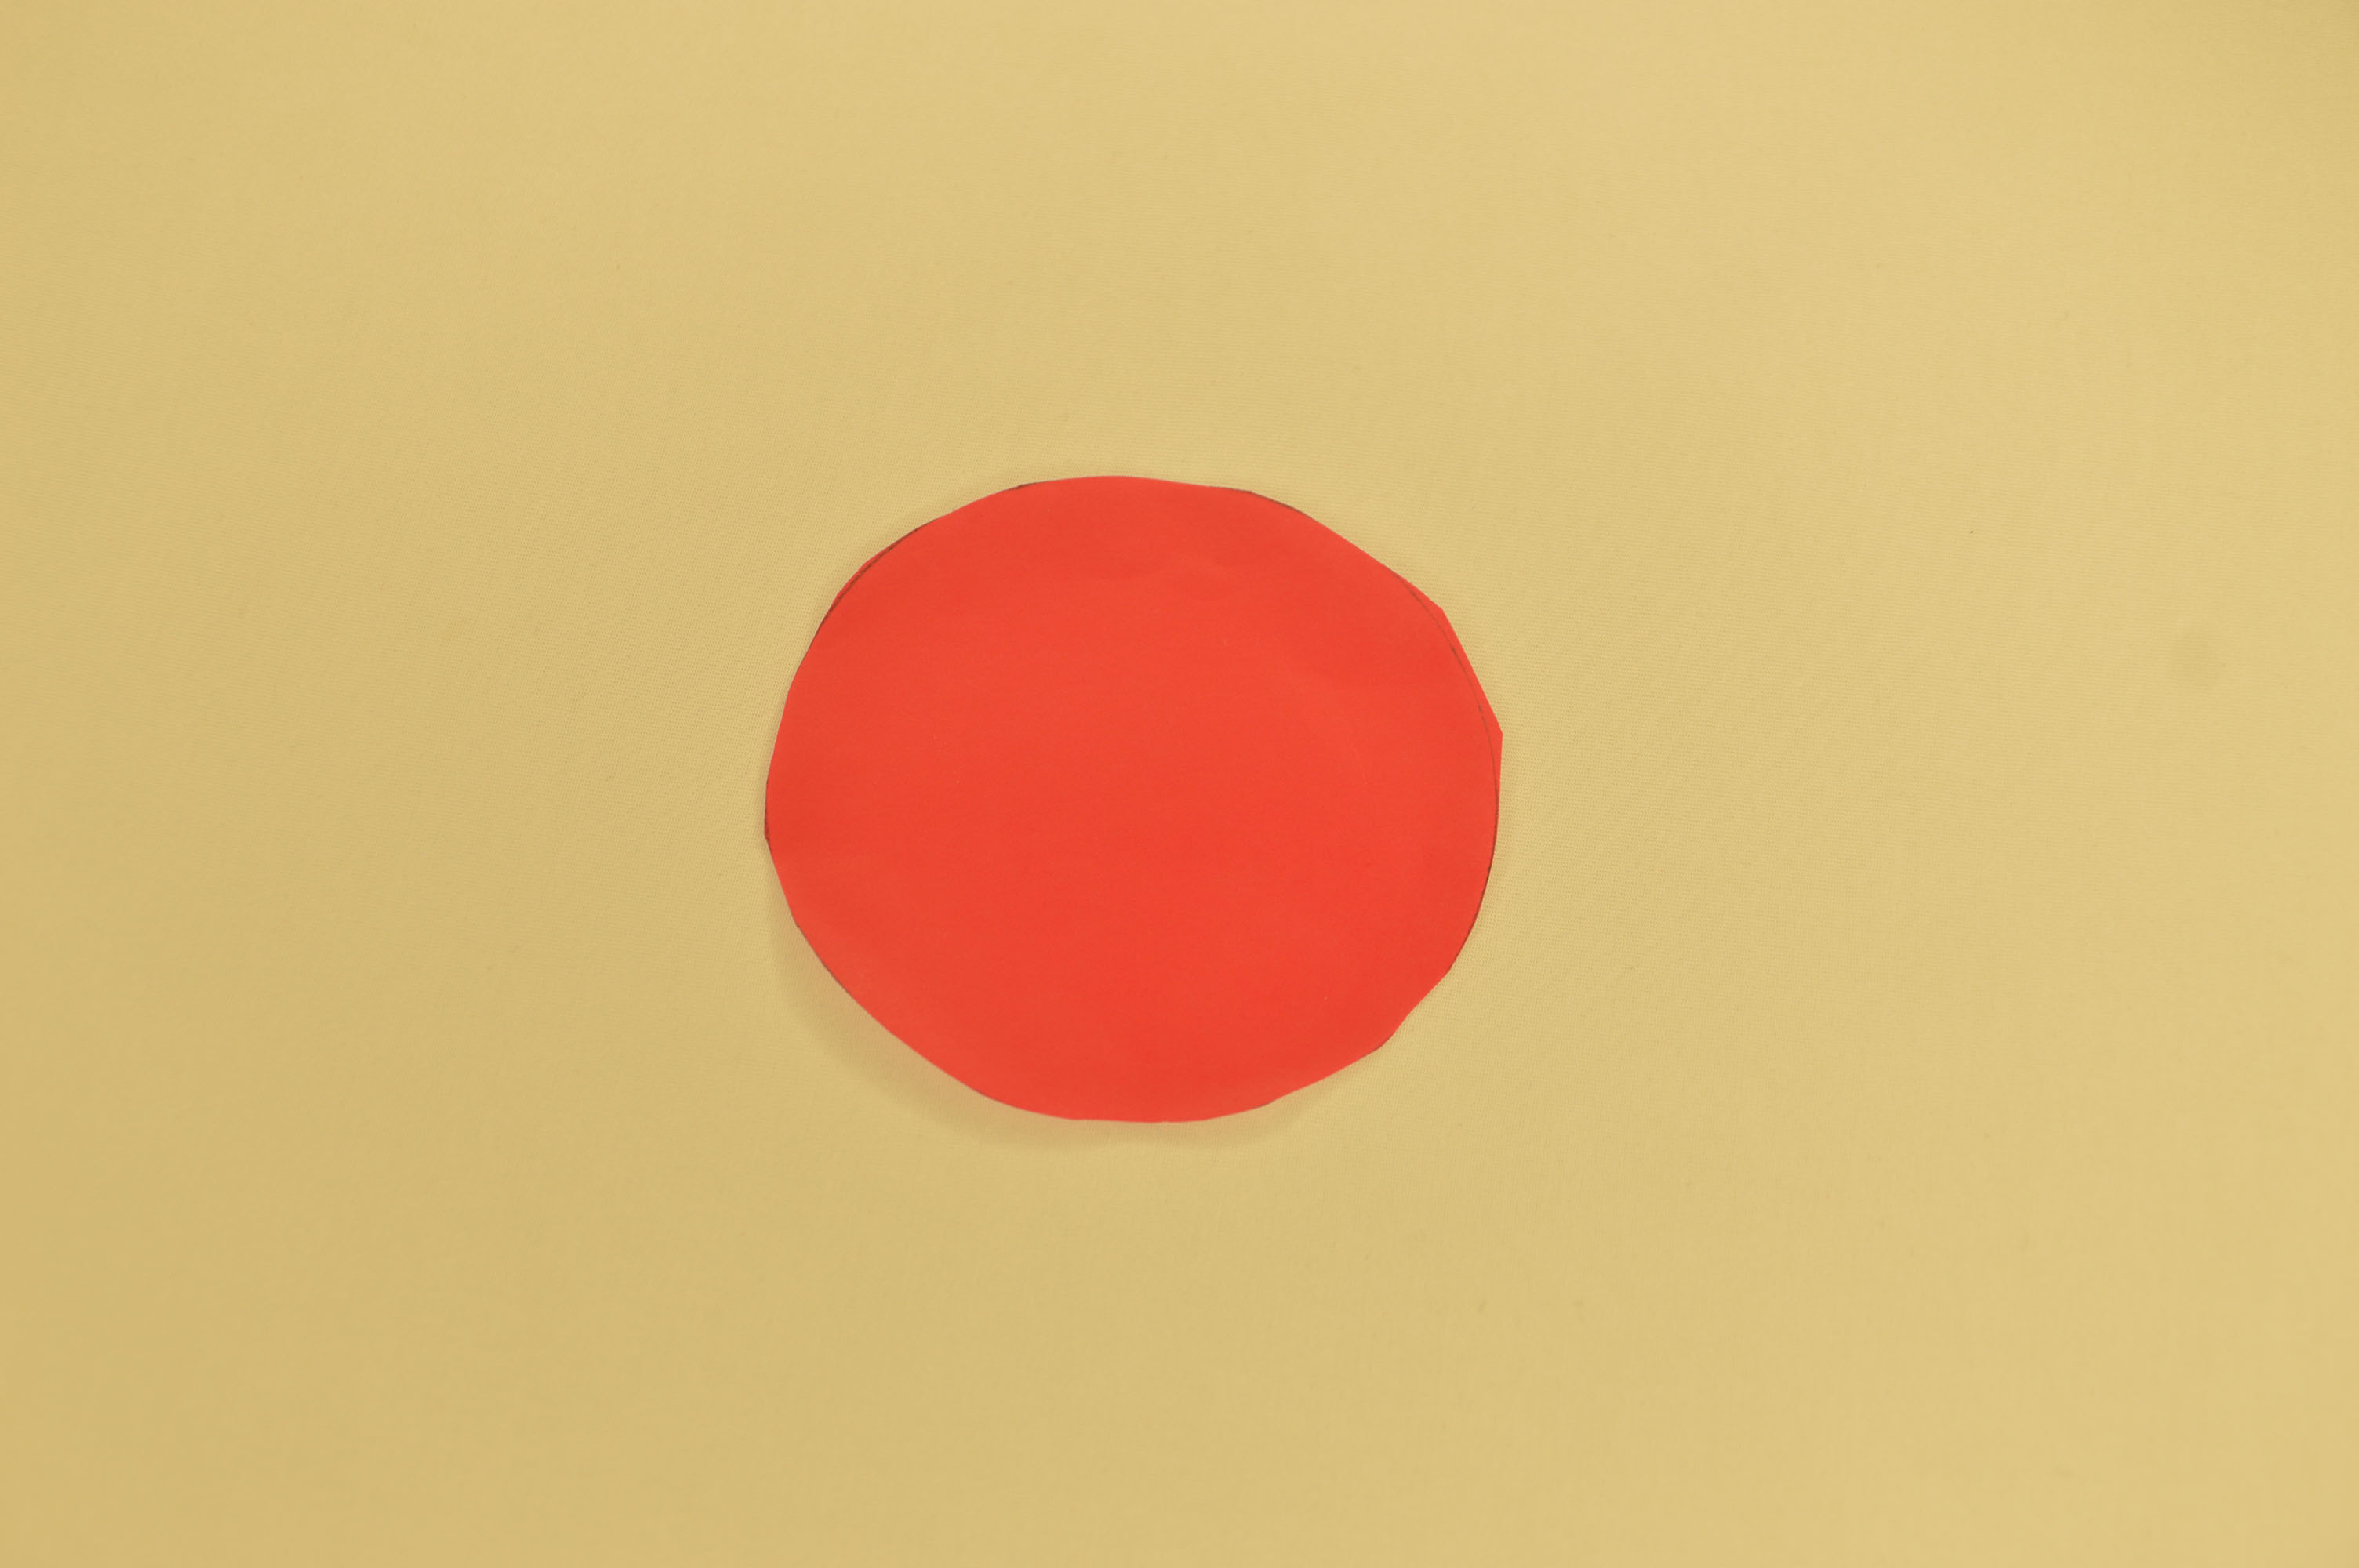
\includegraphics[width=.20\linewidth]{images/train04.jpg} \\
		\vspace{3pt}
		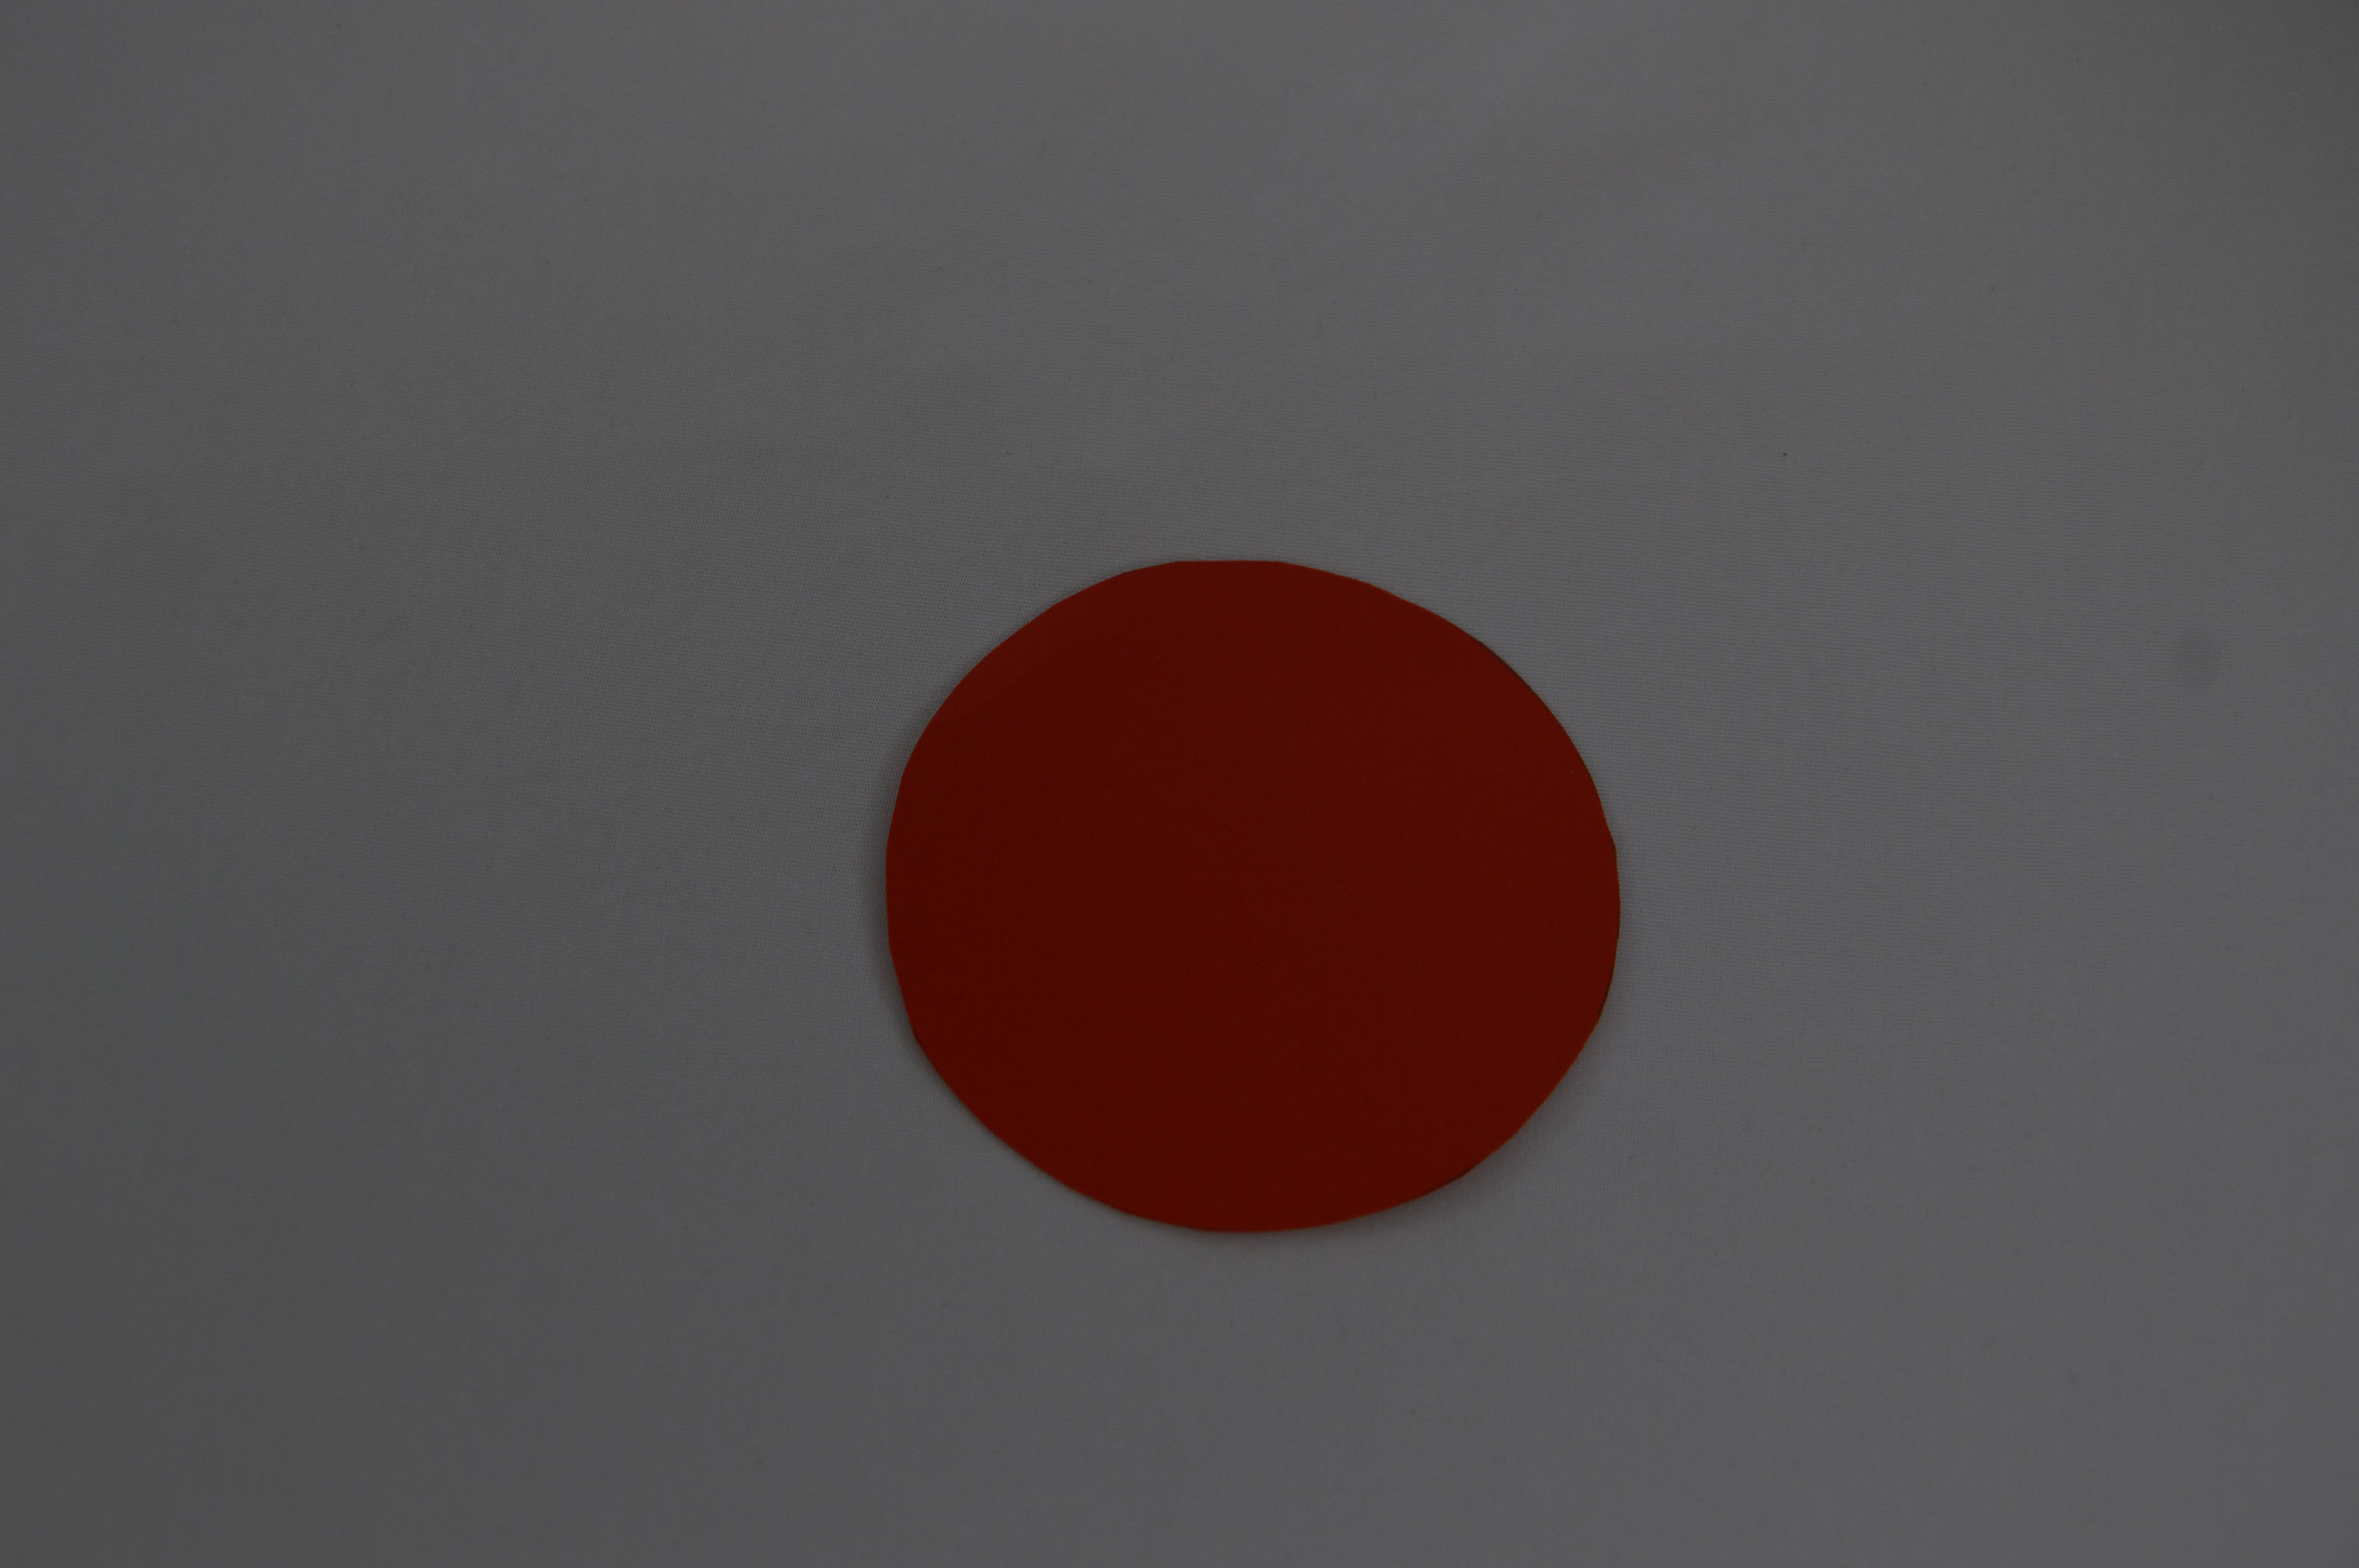
\includegraphics[width=.20\linewidth]{images/train05.jpg}
		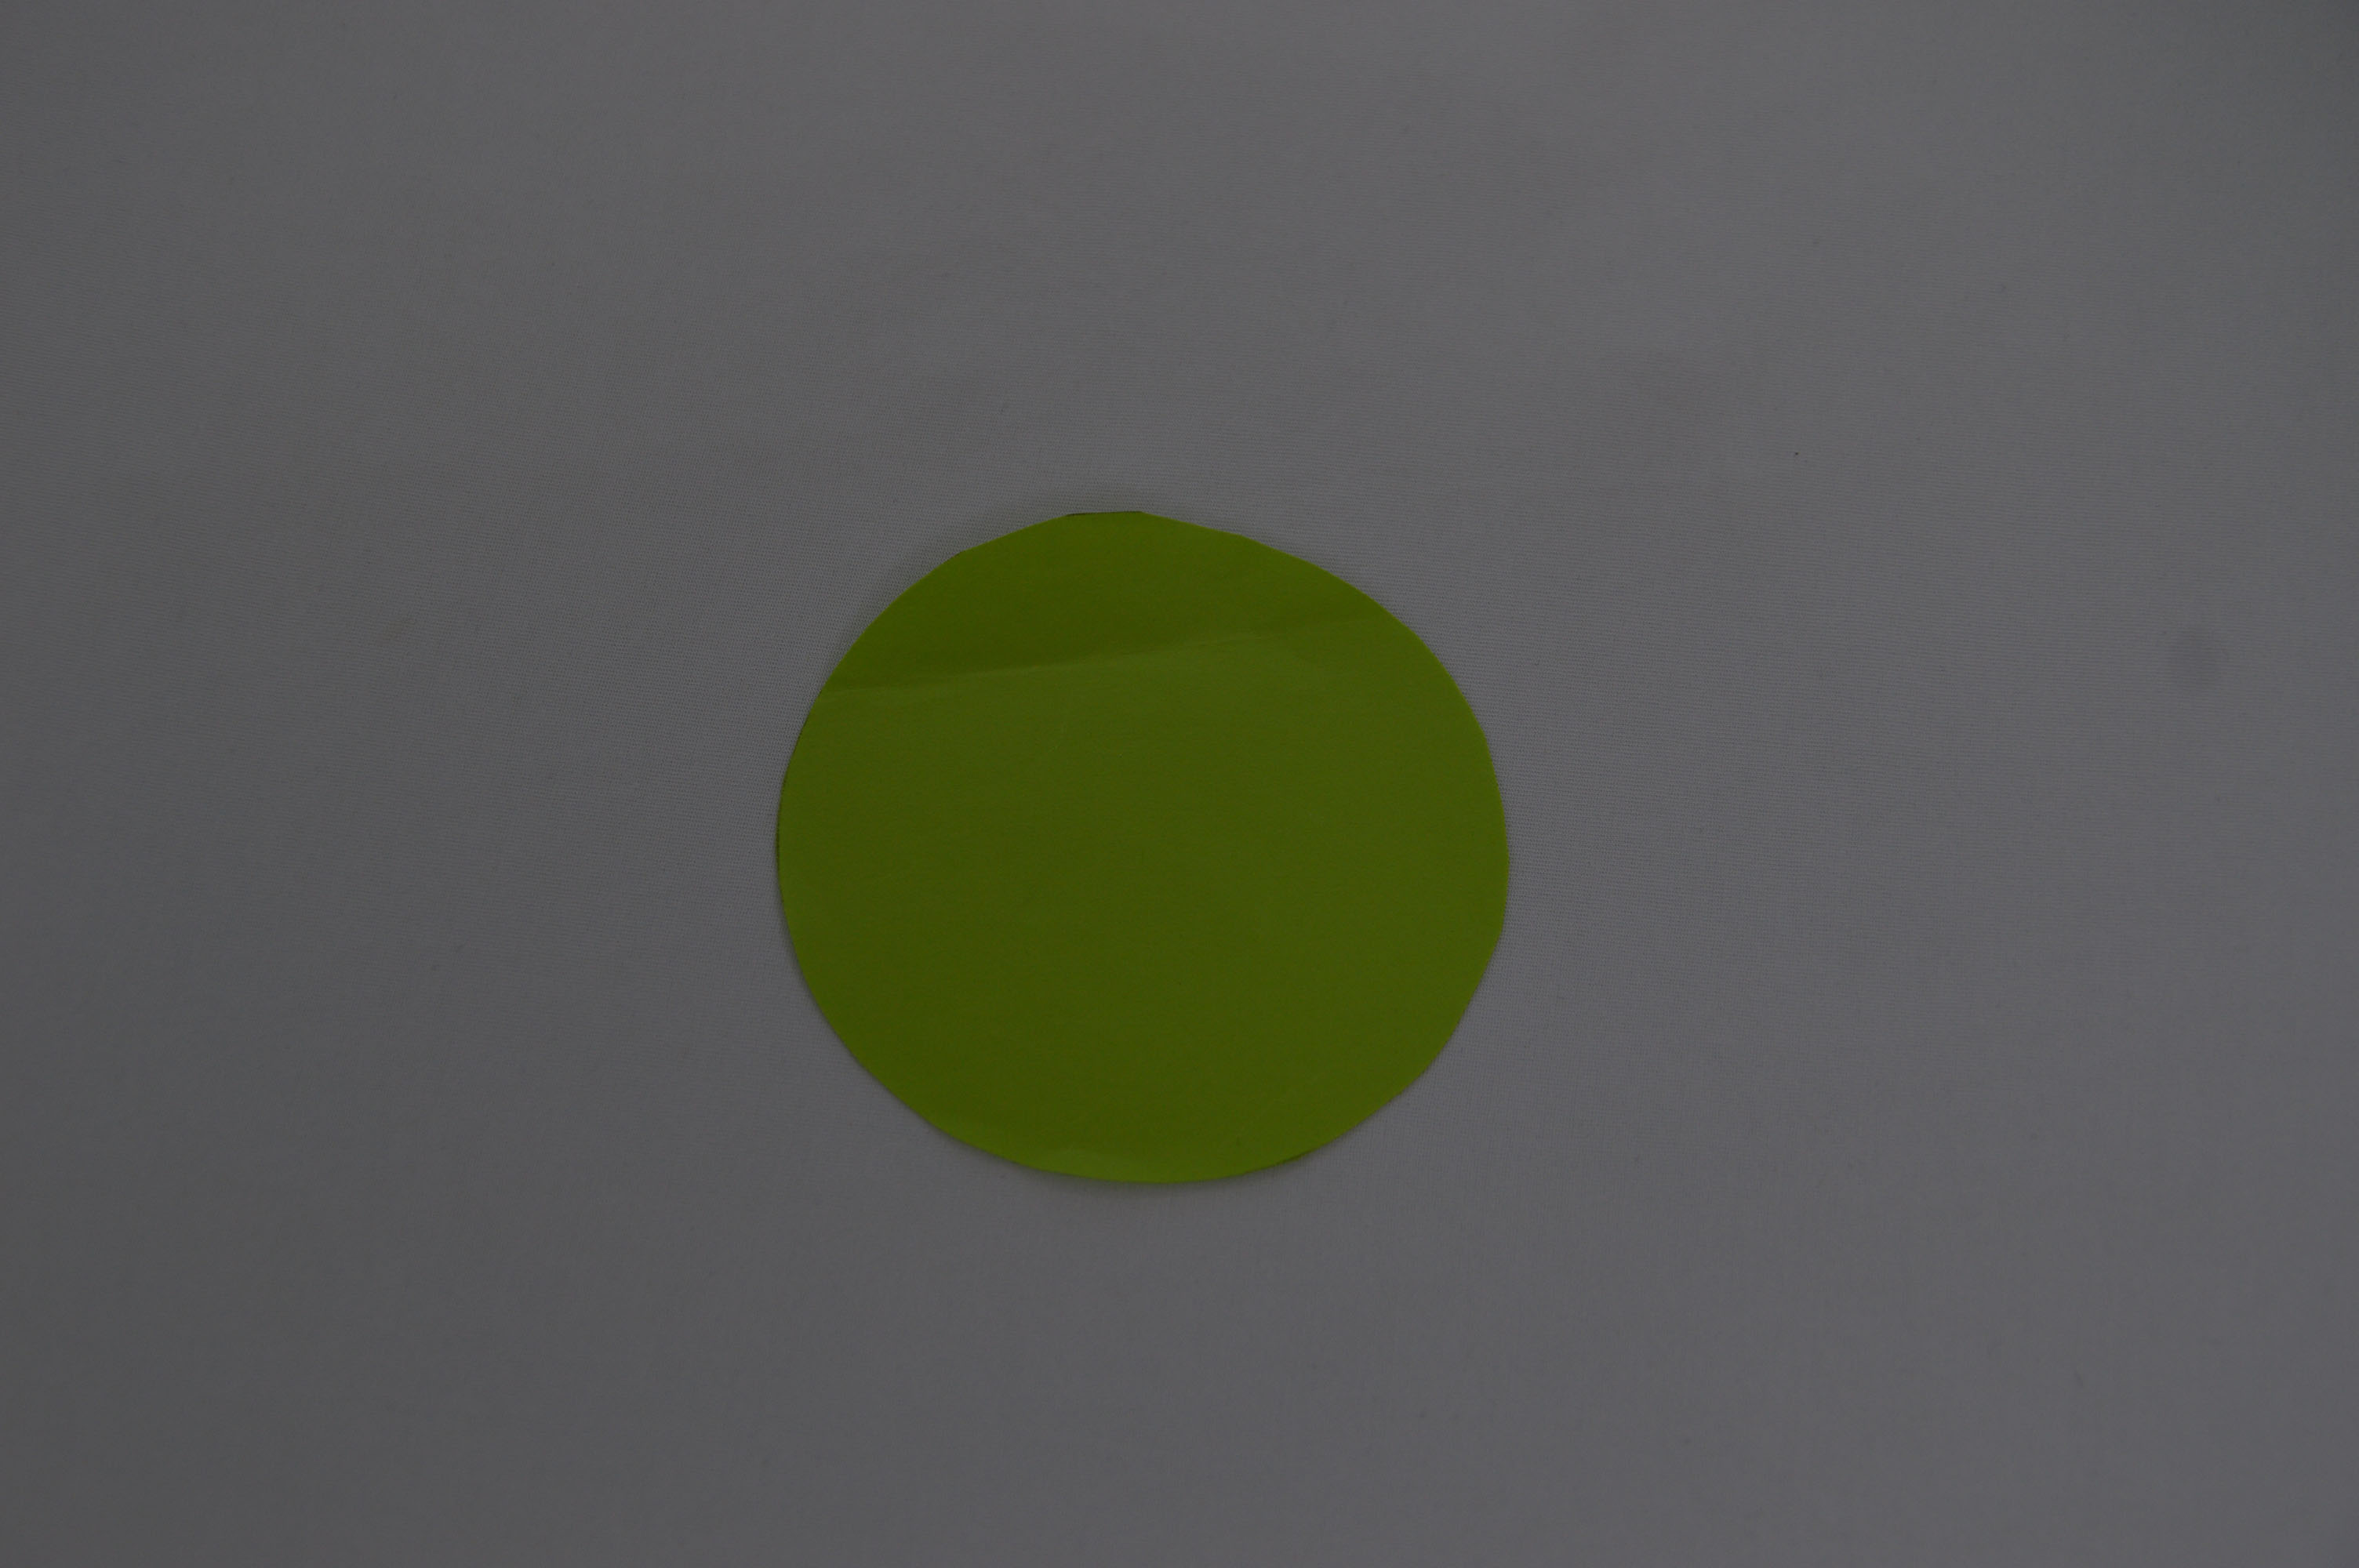
\includegraphics[width=.20\linewidth]{images/train06.jpg}
		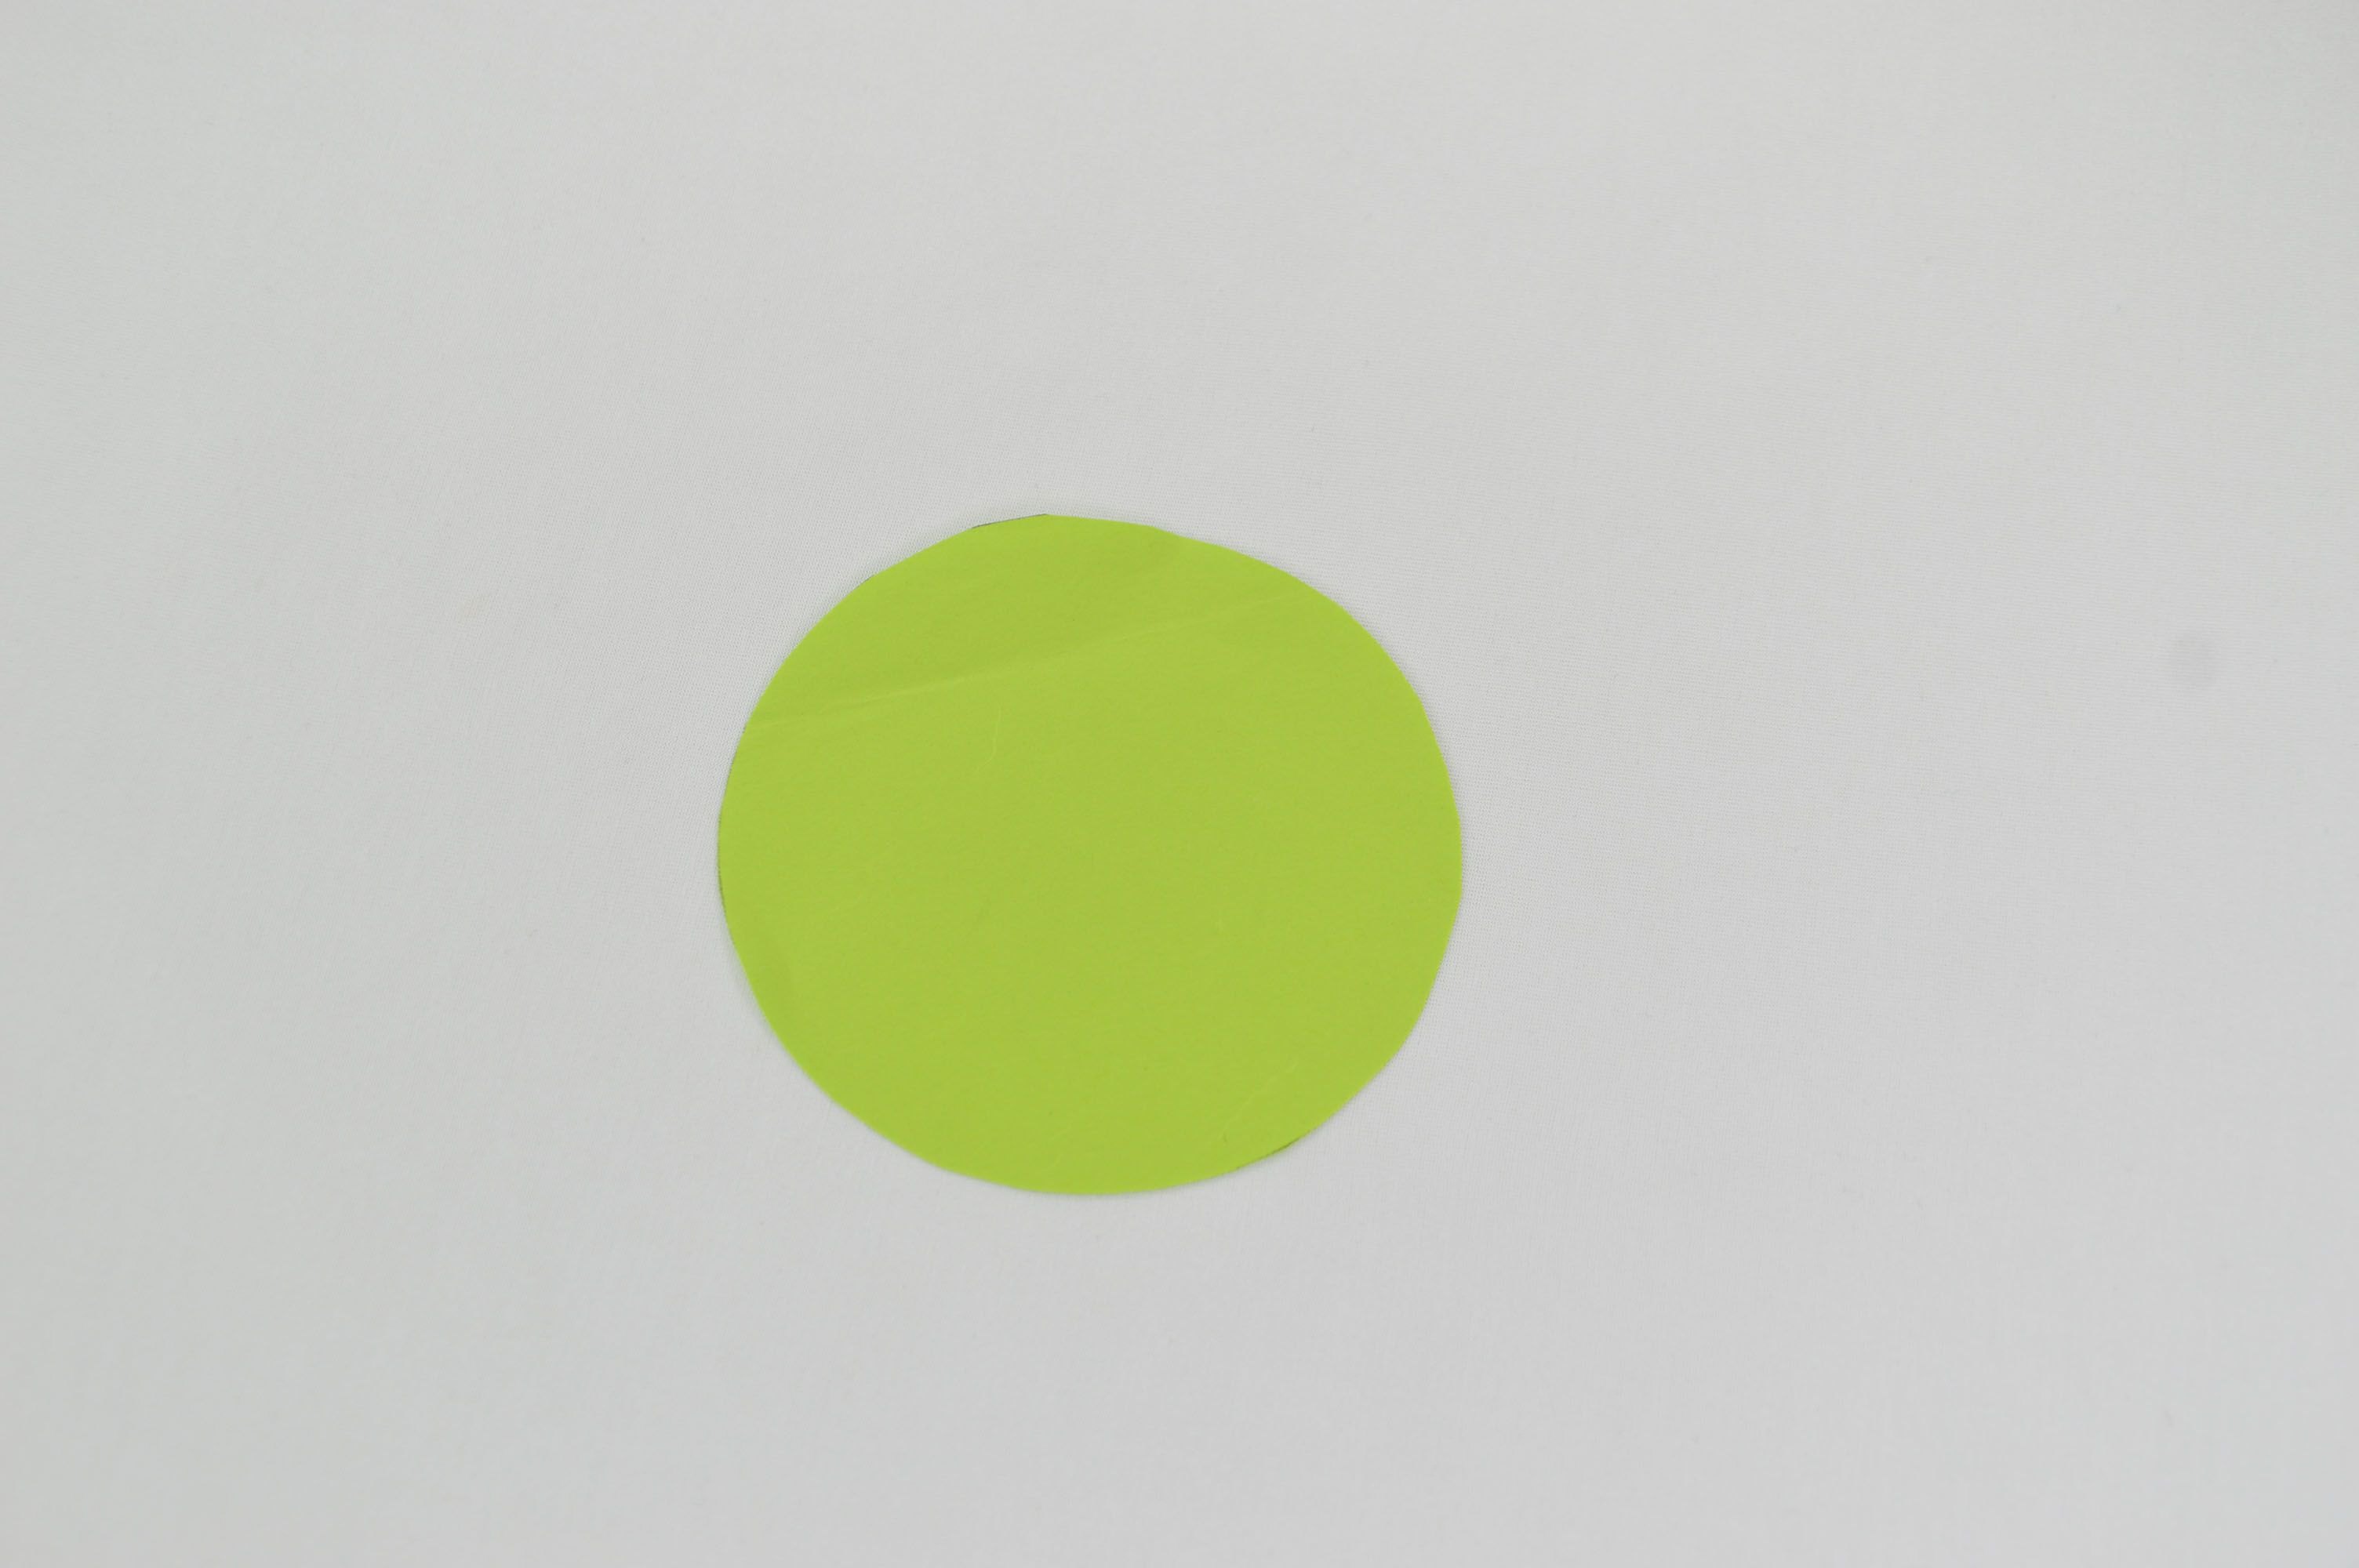
\includegraphics[width=.20\linewidth]{images/train07.jpg}
		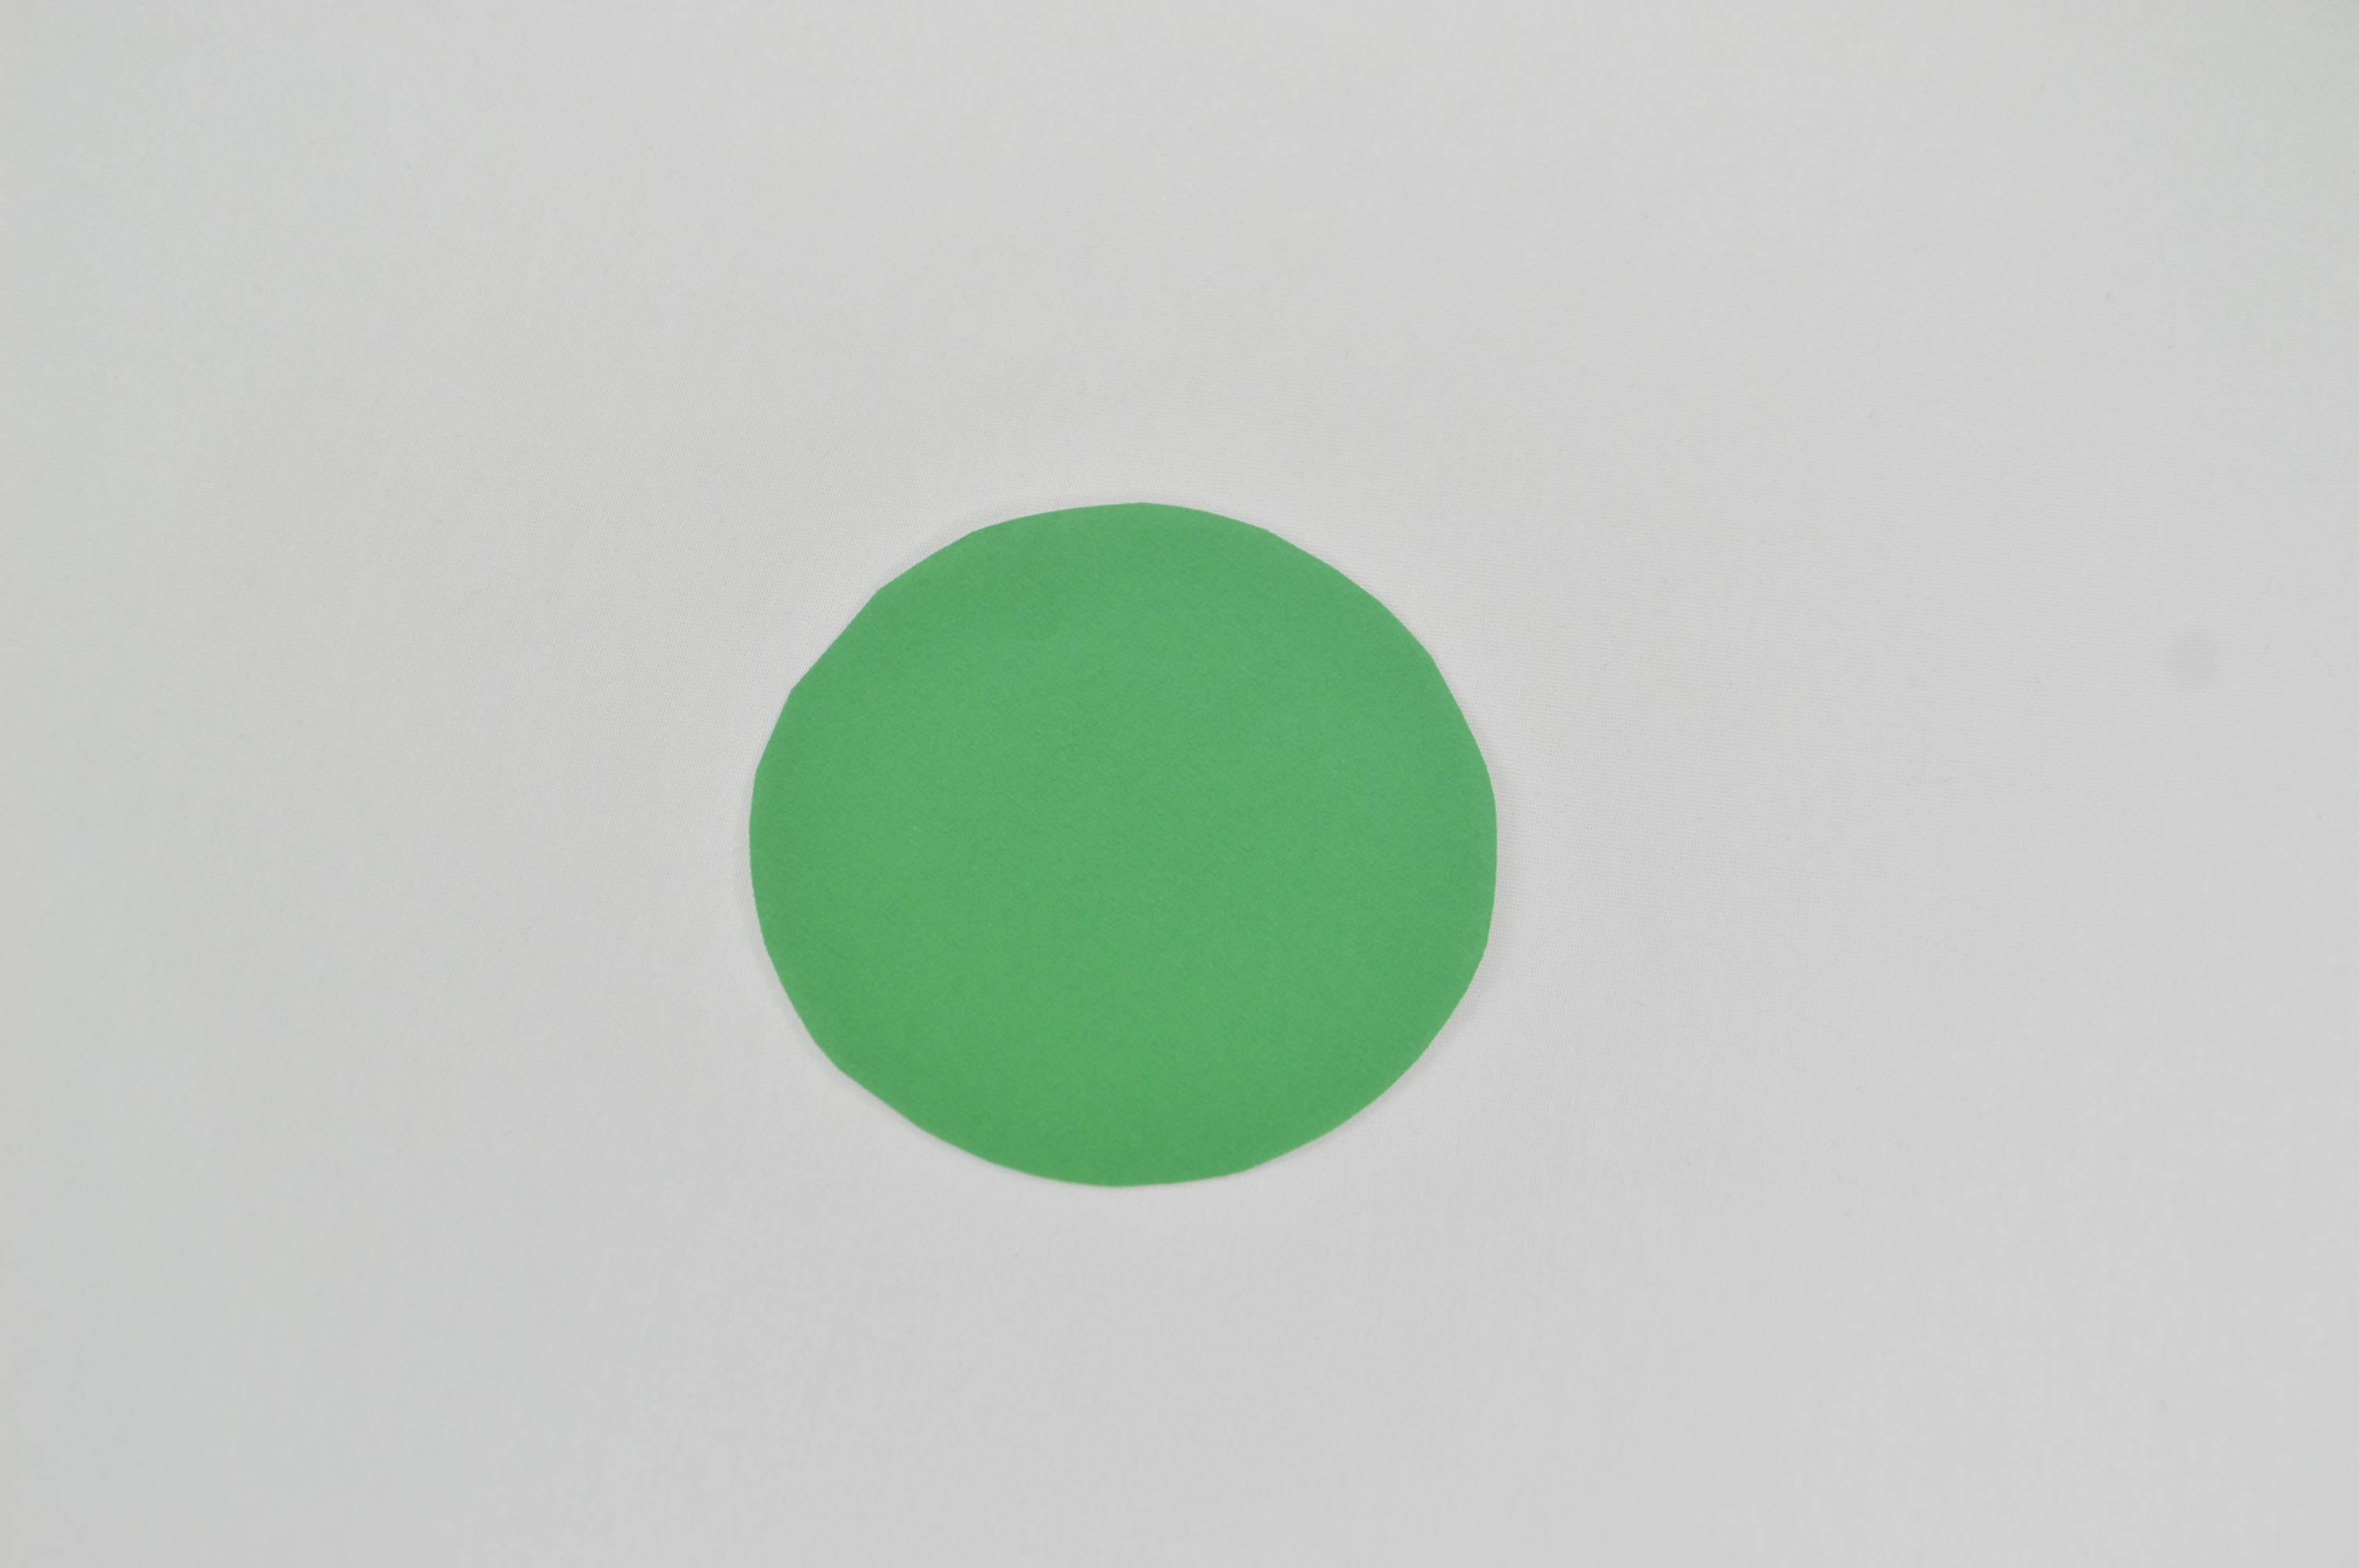
\includegraphics[width=.20\linewidth]{images/train08.jpg}
		\caption{First set of photos}
	\end{figure}

	For the second set of images, we took photos of single coloured cylinders from different sides with a "fixed" light source, the sun. All the cyliners had roughly the same diameter as they were created by wrapping paper around a plastic bottle. We used paper of different shades of each colour and of different textures. \\
	
	Photos were taken when the sun was low, so the light was hitting the cylinder more horizontally than vertically. Pictures were taken from 3 viewing points - towards the sunlight, against the sunlight and perpendicular to the sunlight. This ensured somewhat gradient distribution of the cololor in the images. This is important, because cylinders that the robot will encounter will also have gradient distribution of the color.\\
	
	We obtained around 130 photos of this kind. A subset of the images is included below.
	
	\begin{figure}[H]
		\centering
		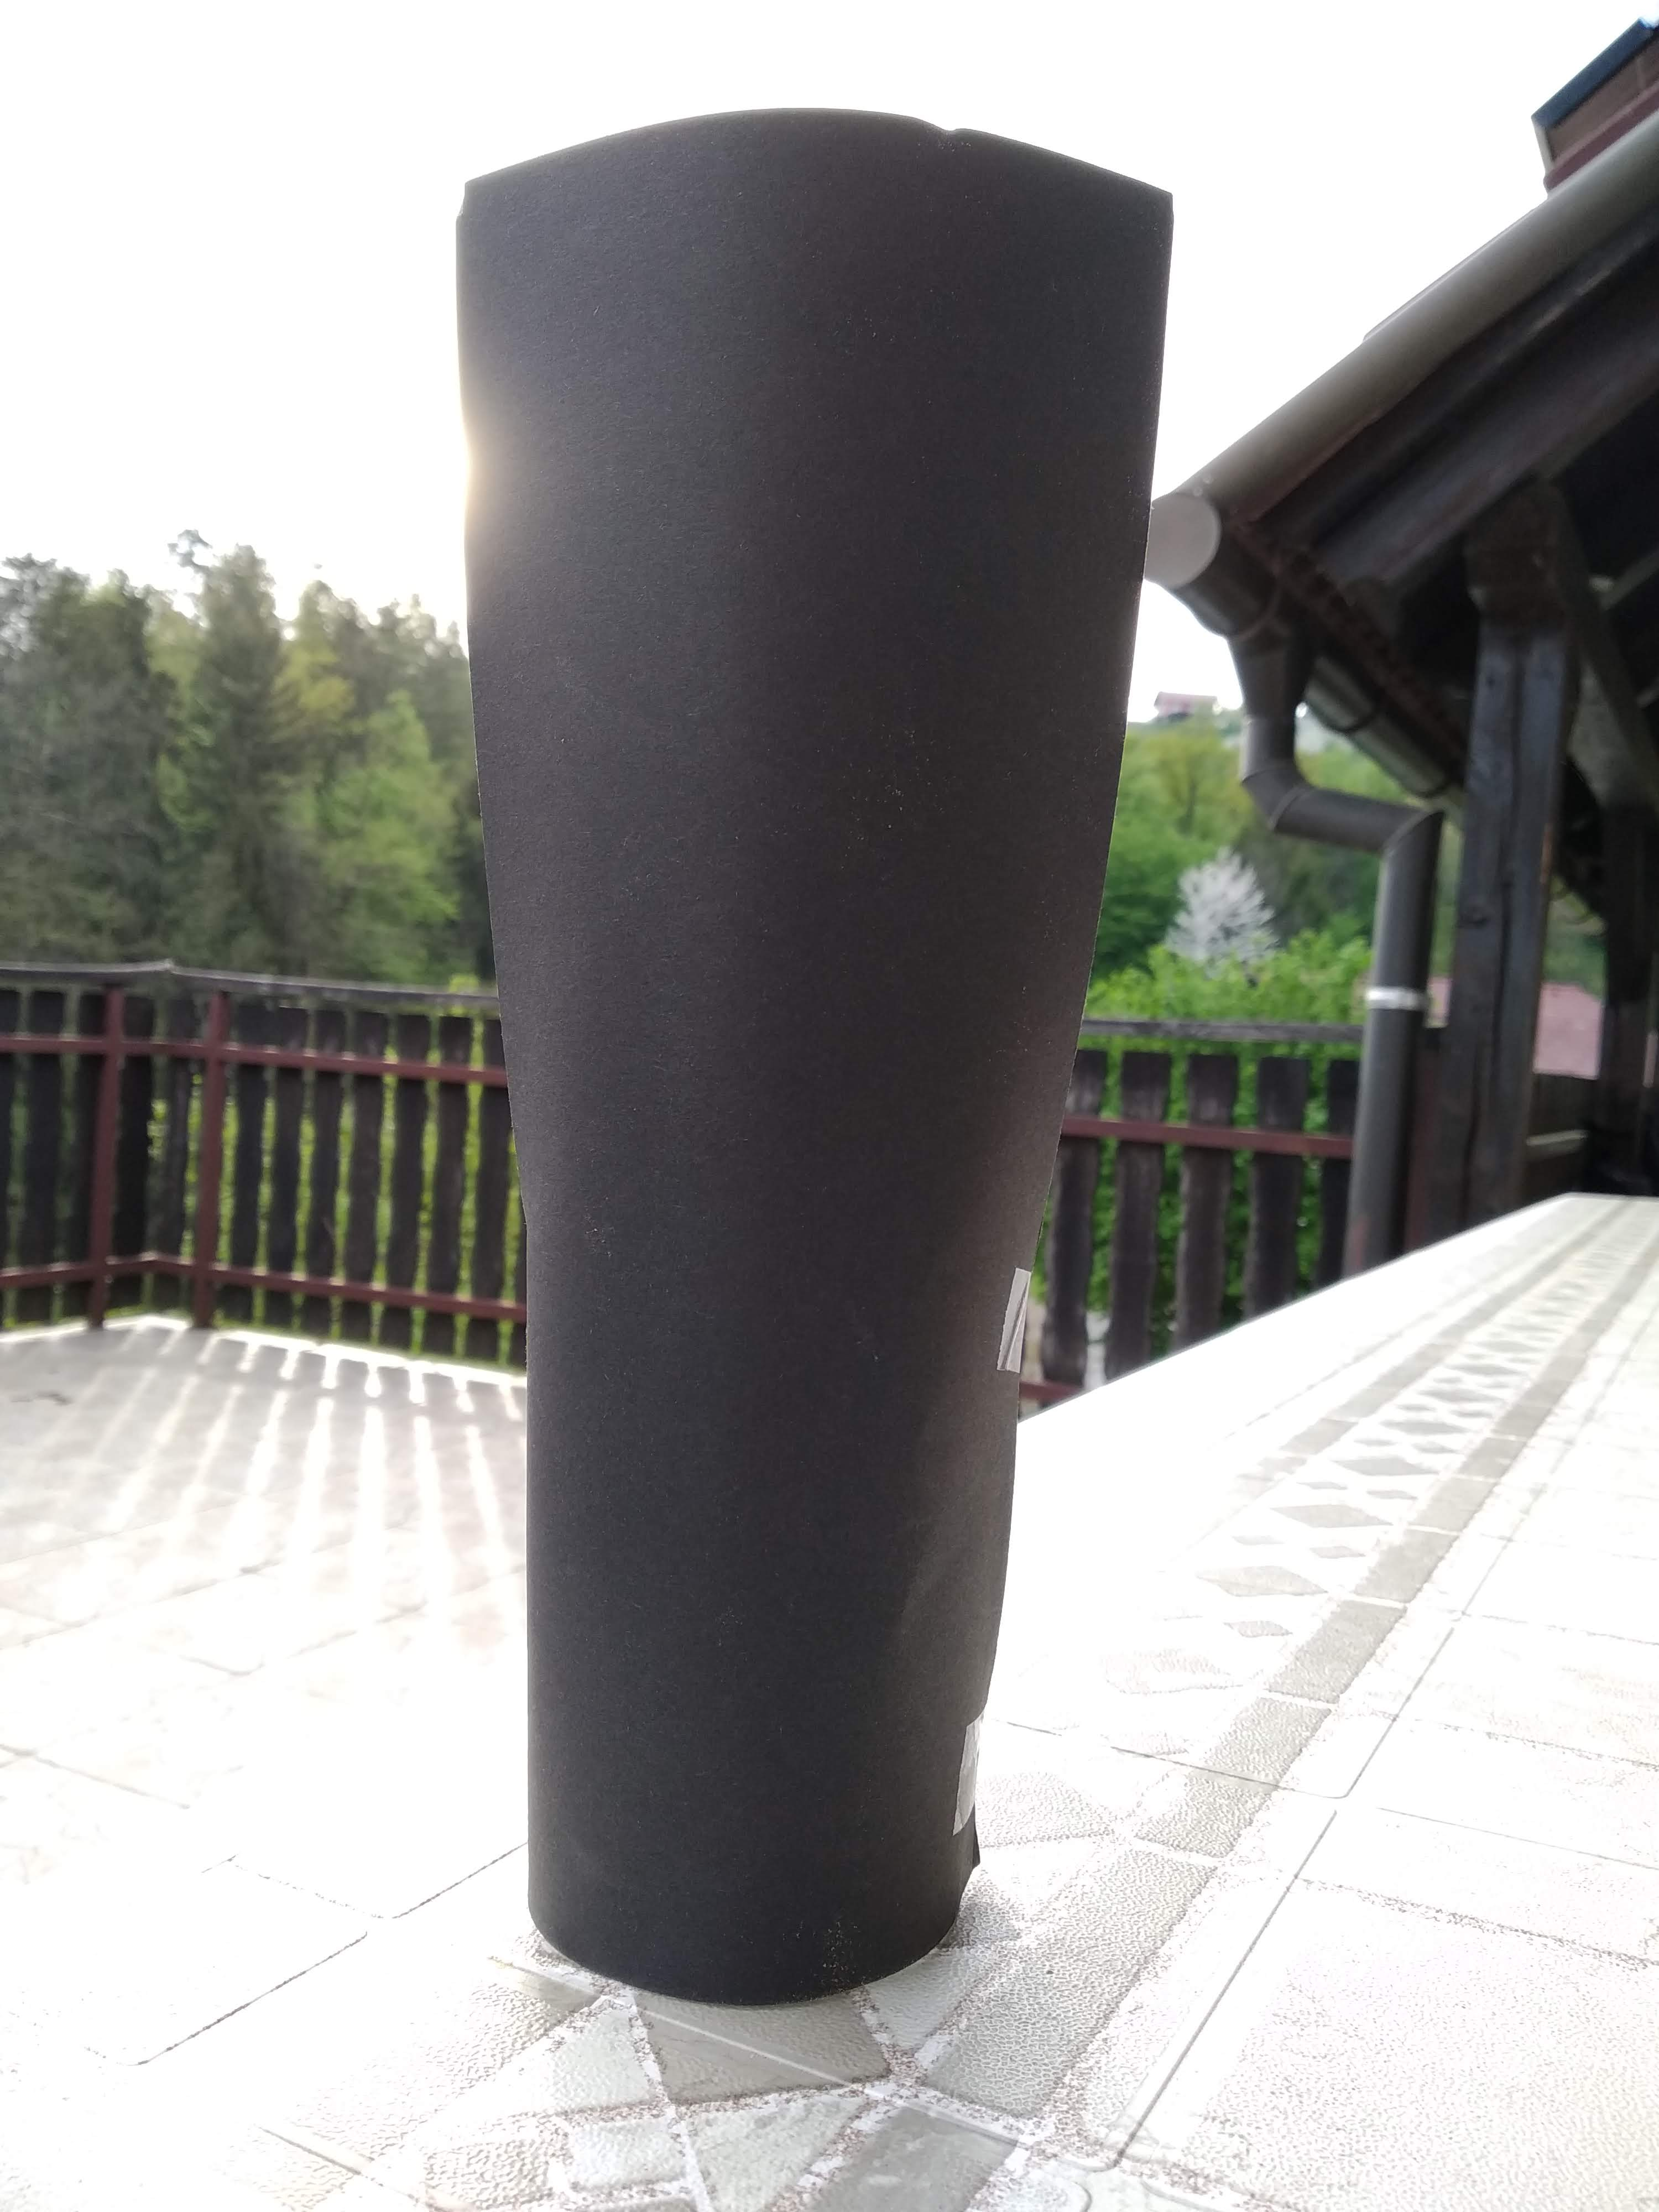
\includegraphics[width=.13\linewidth]{images/test01.jpg}
		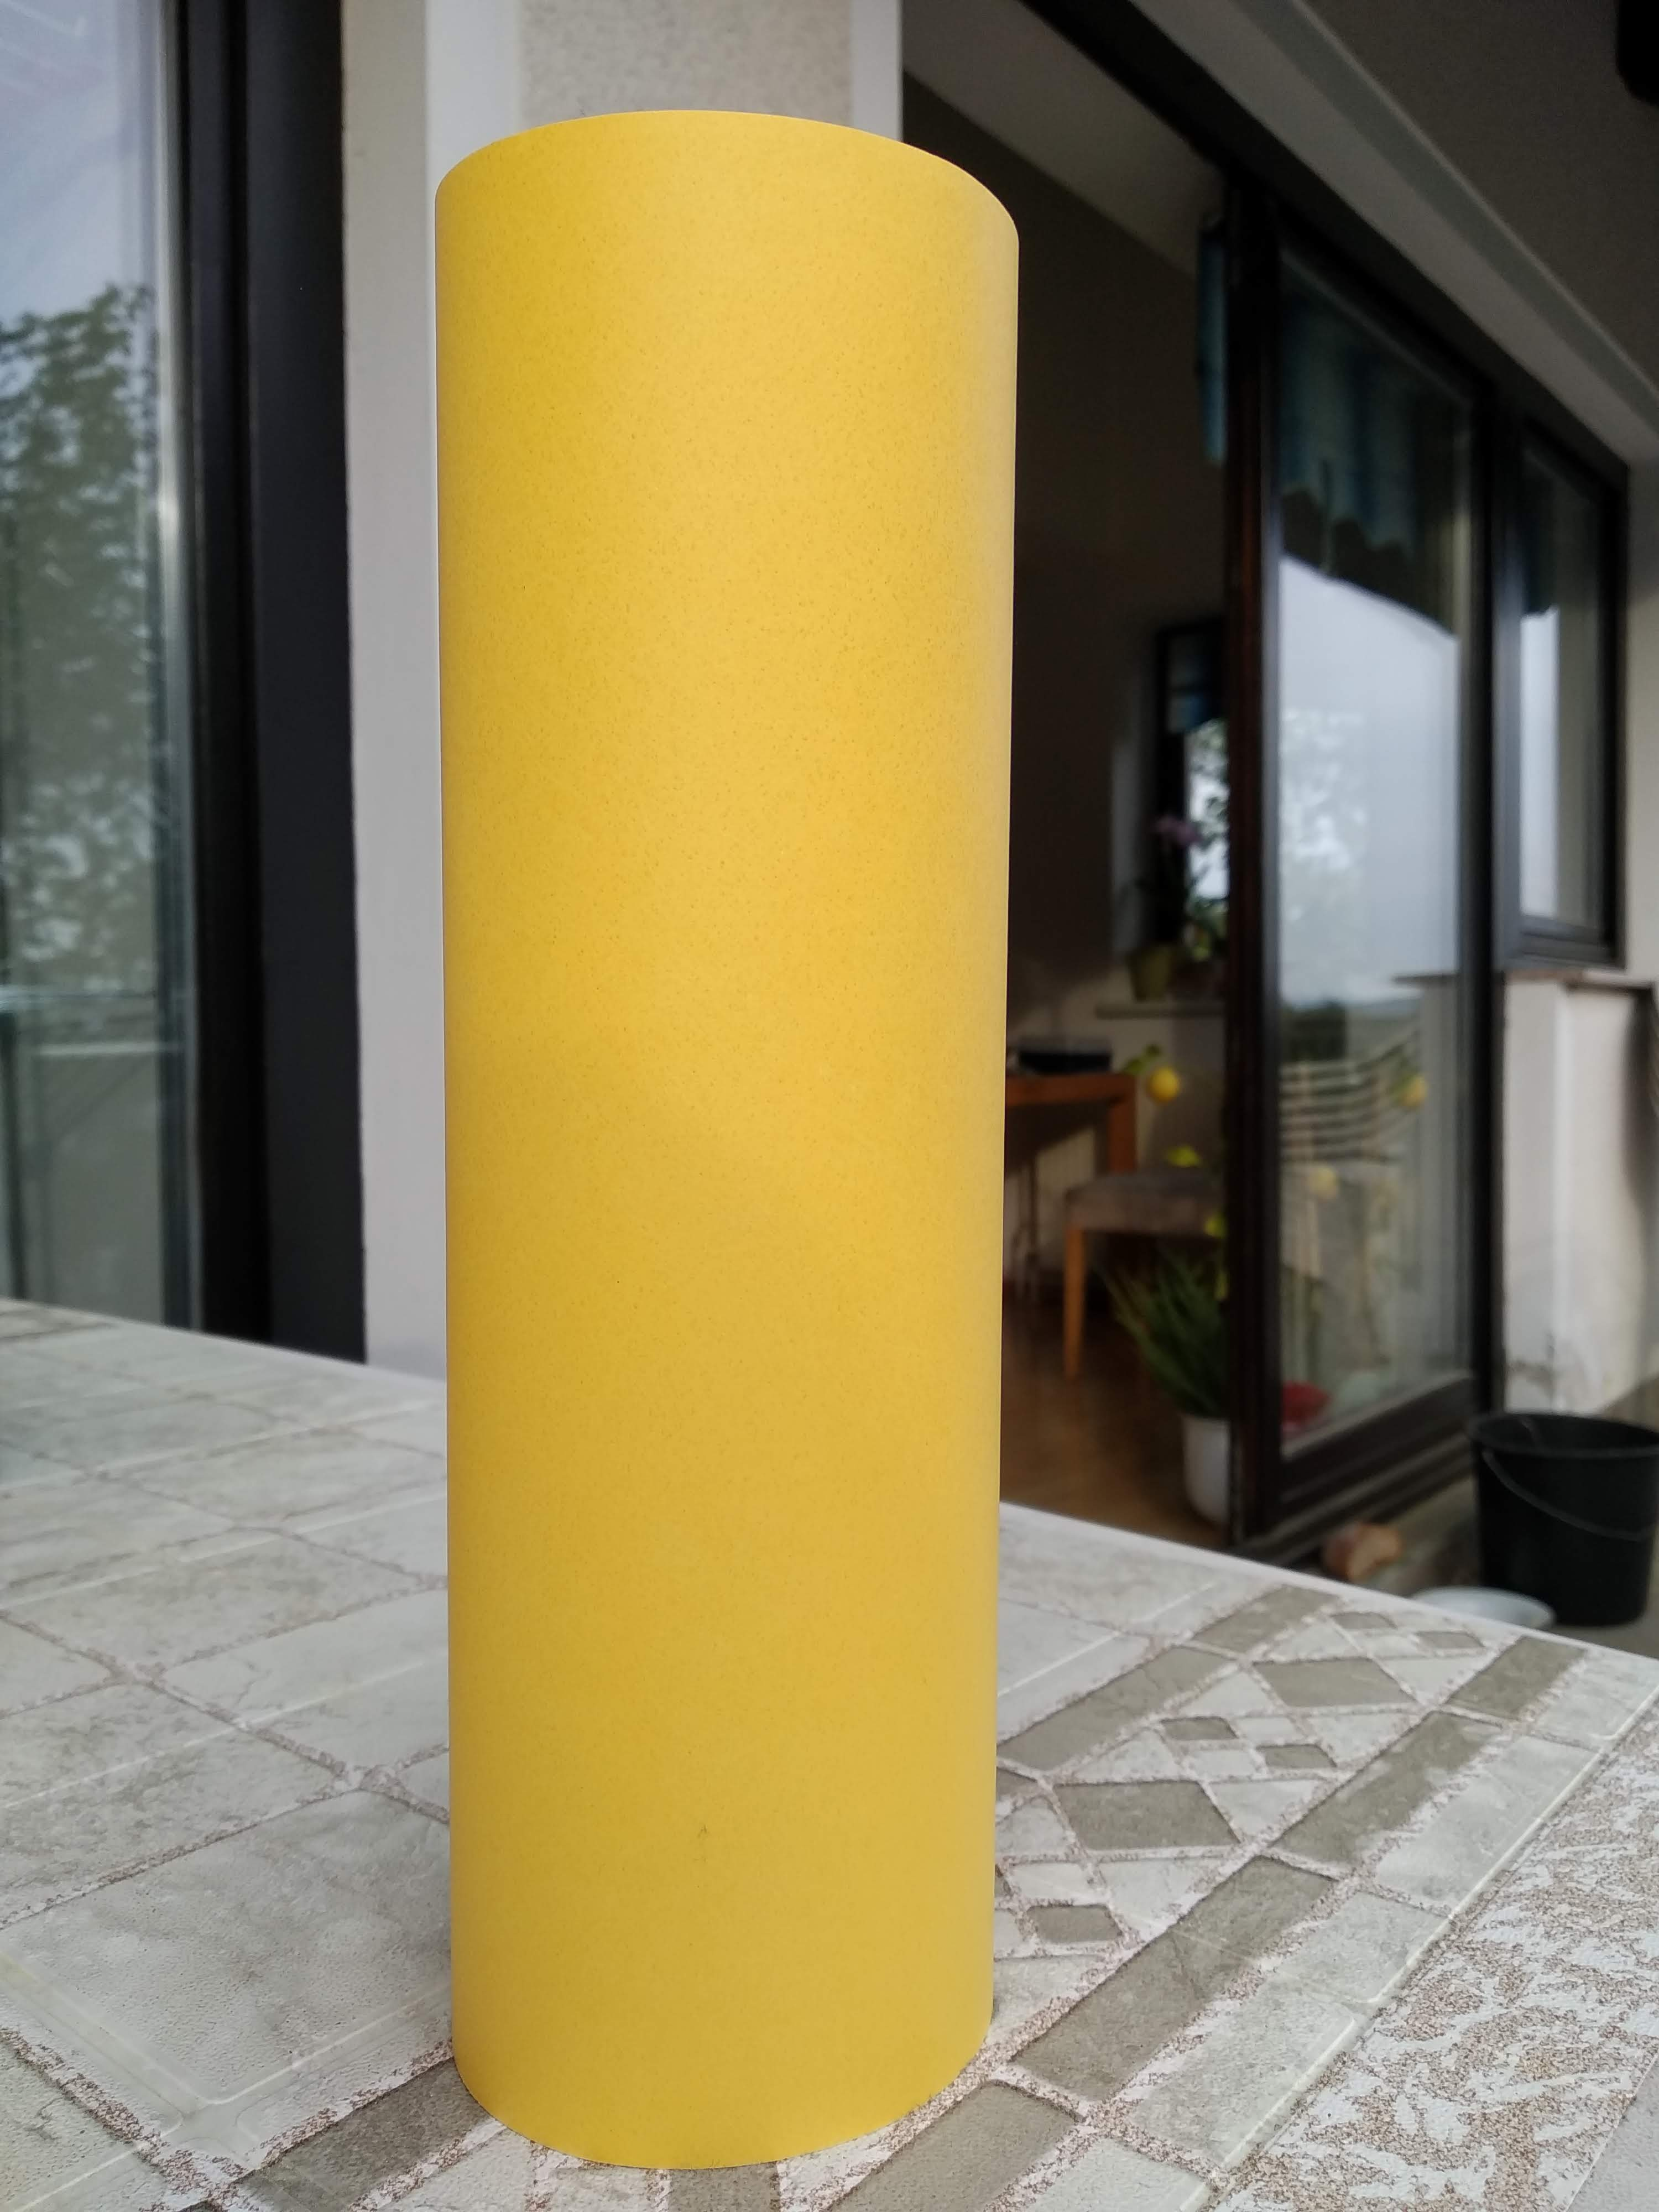
\includegraphics[width=.13\linewidth]{images/test02.jpg}
		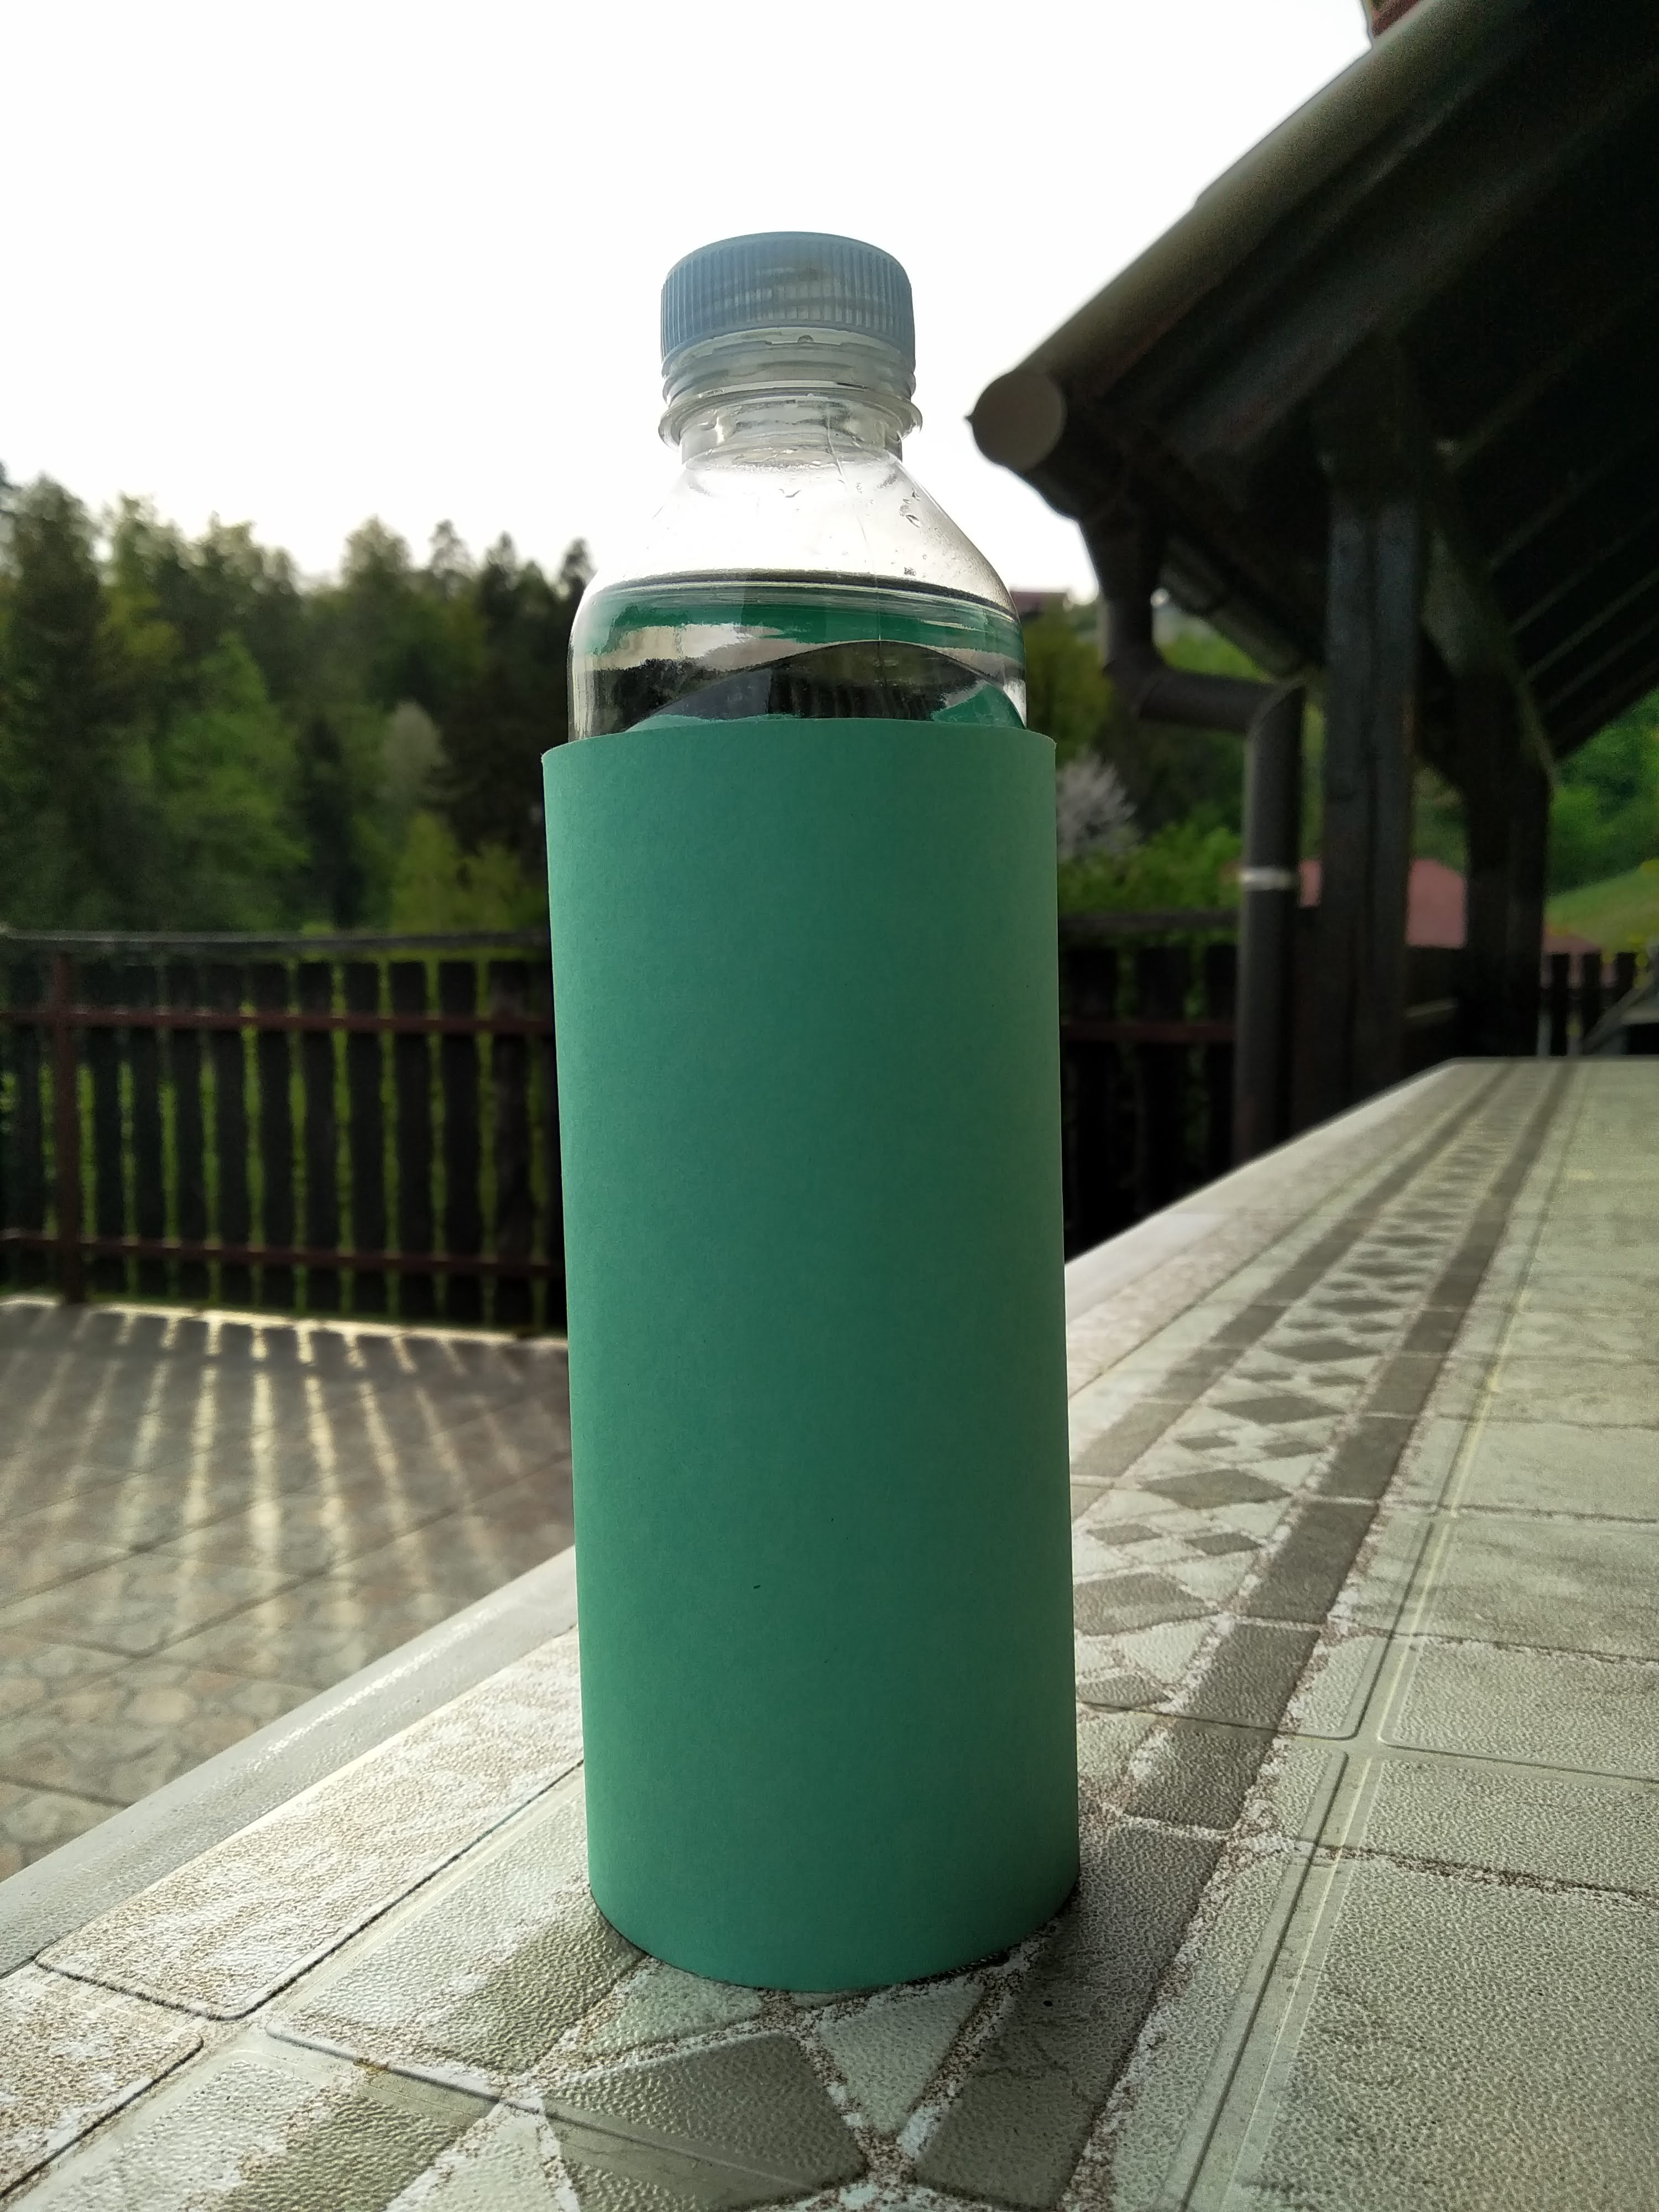
\includegraphics[width=.13\linewidth]{images/test03.jpg}
		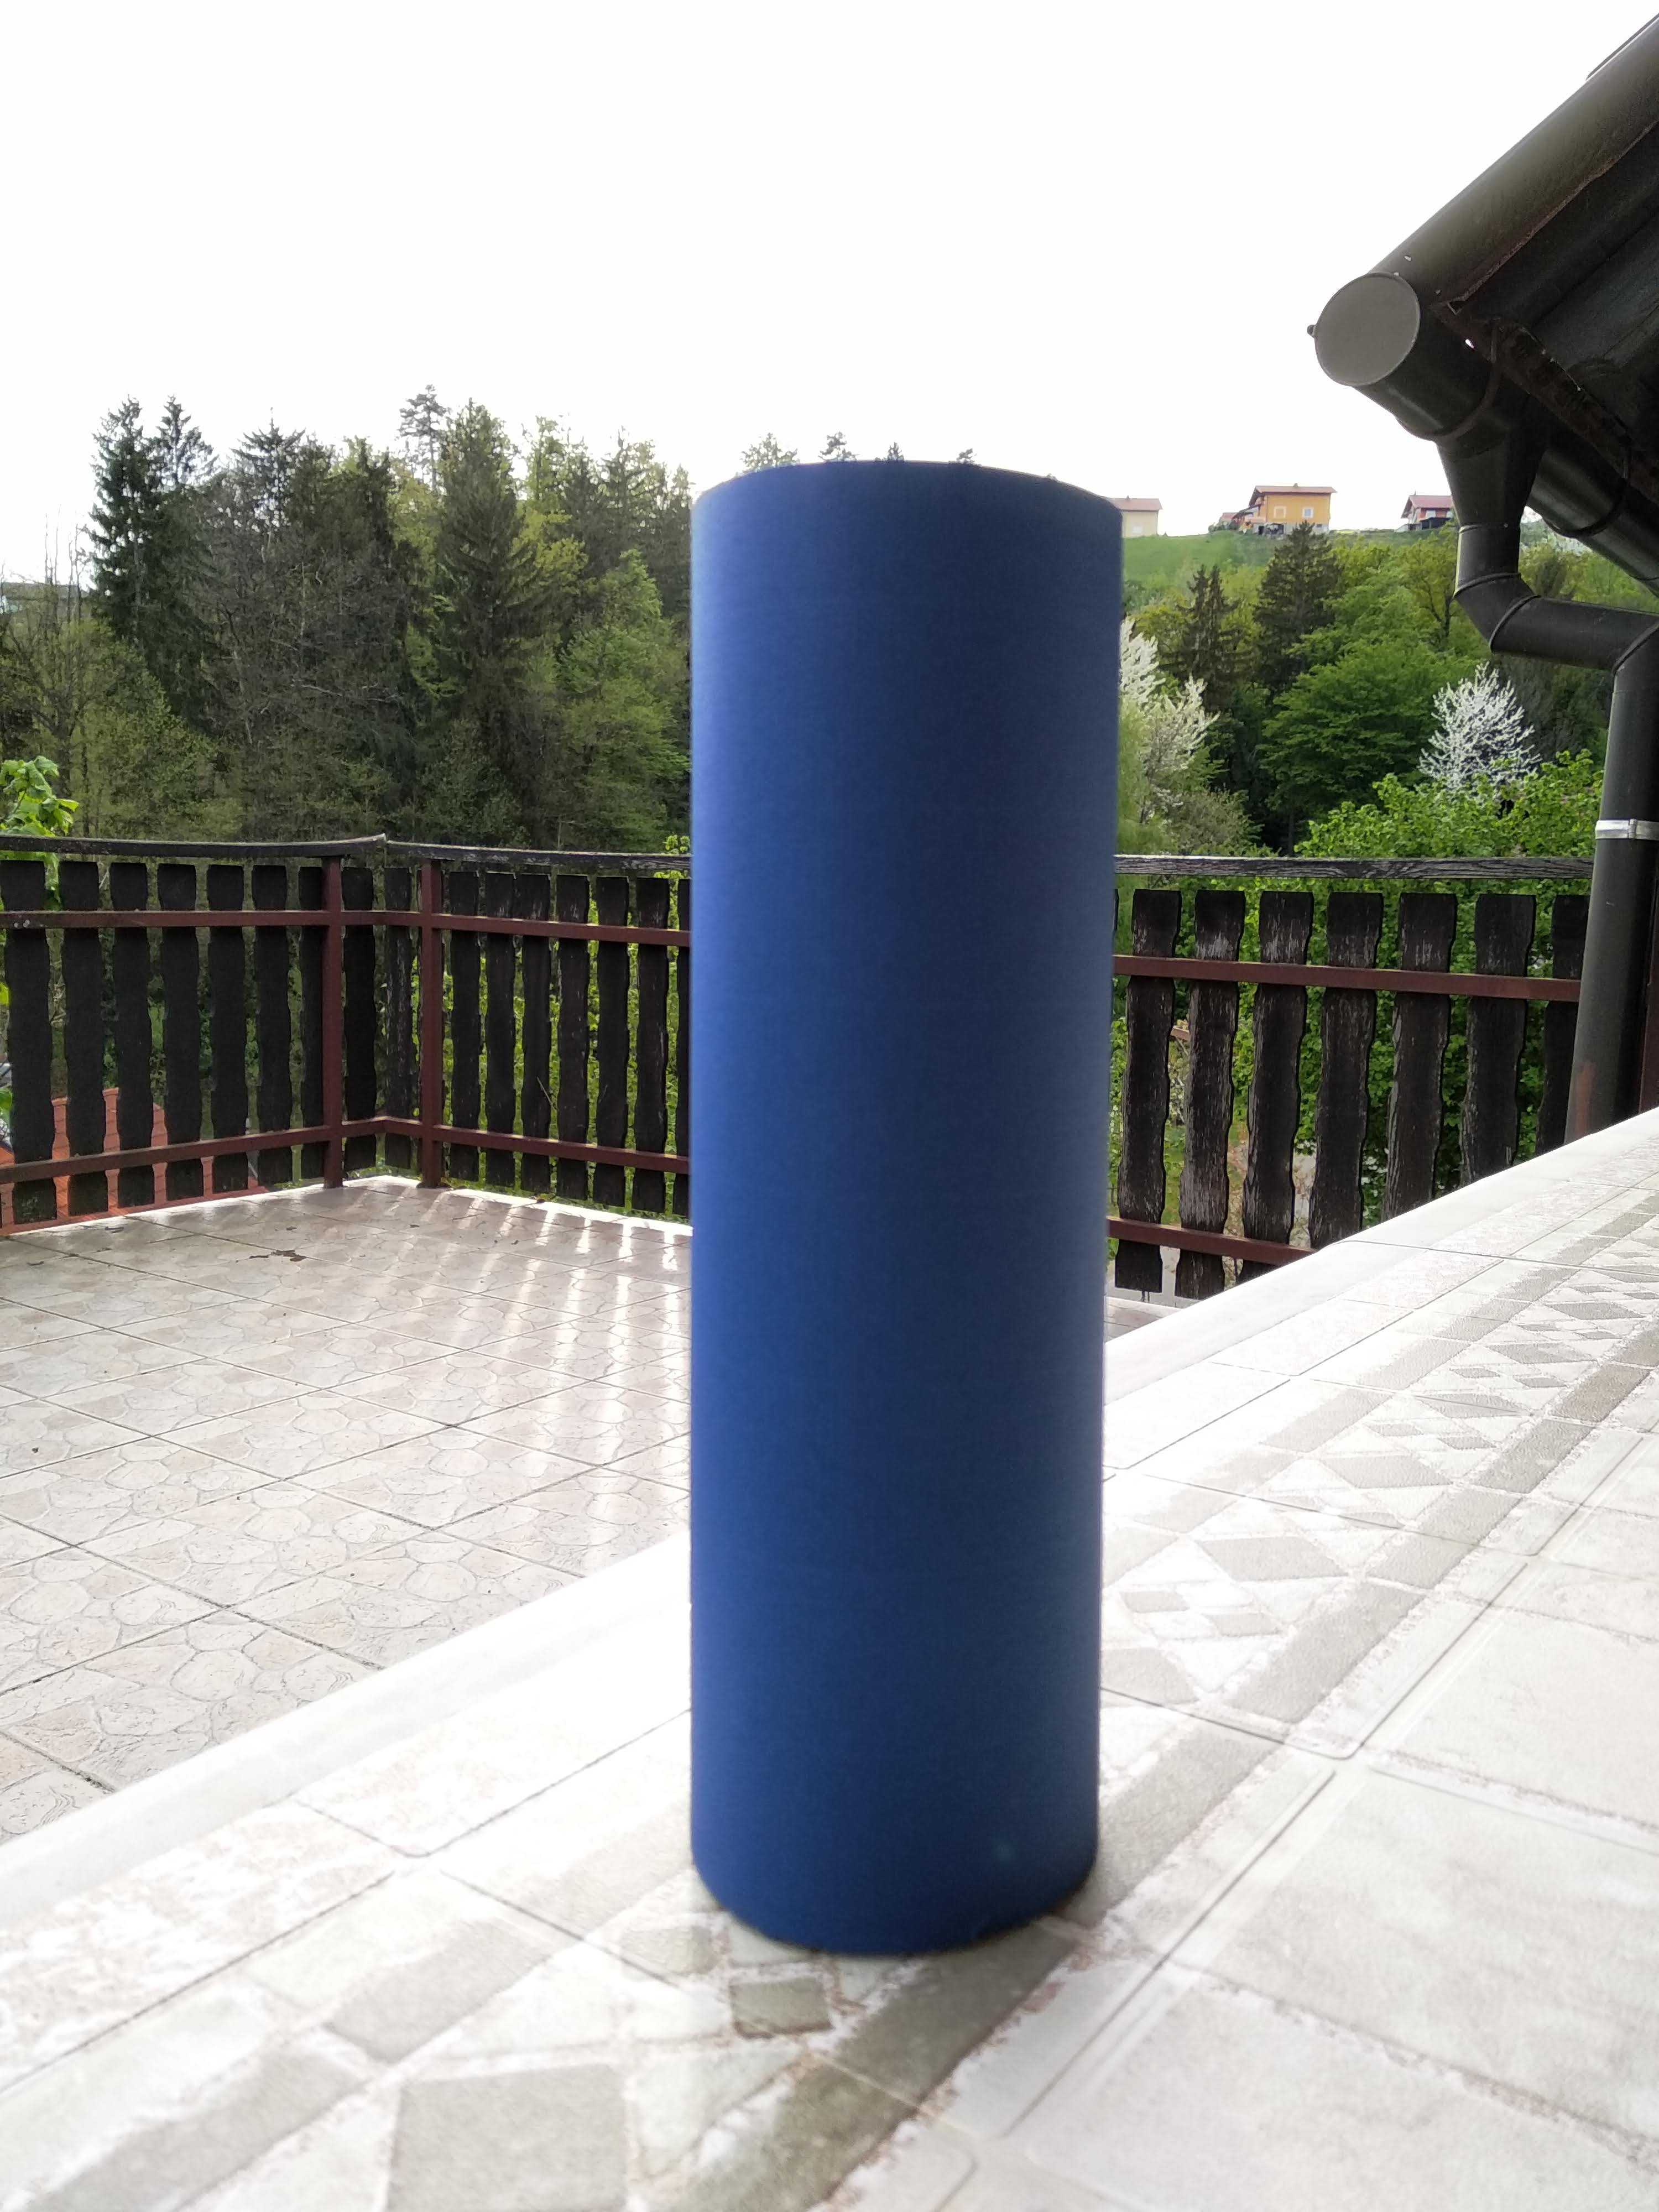
\includegraphics[width=.13\linewidth]{images/test04.jpg}
		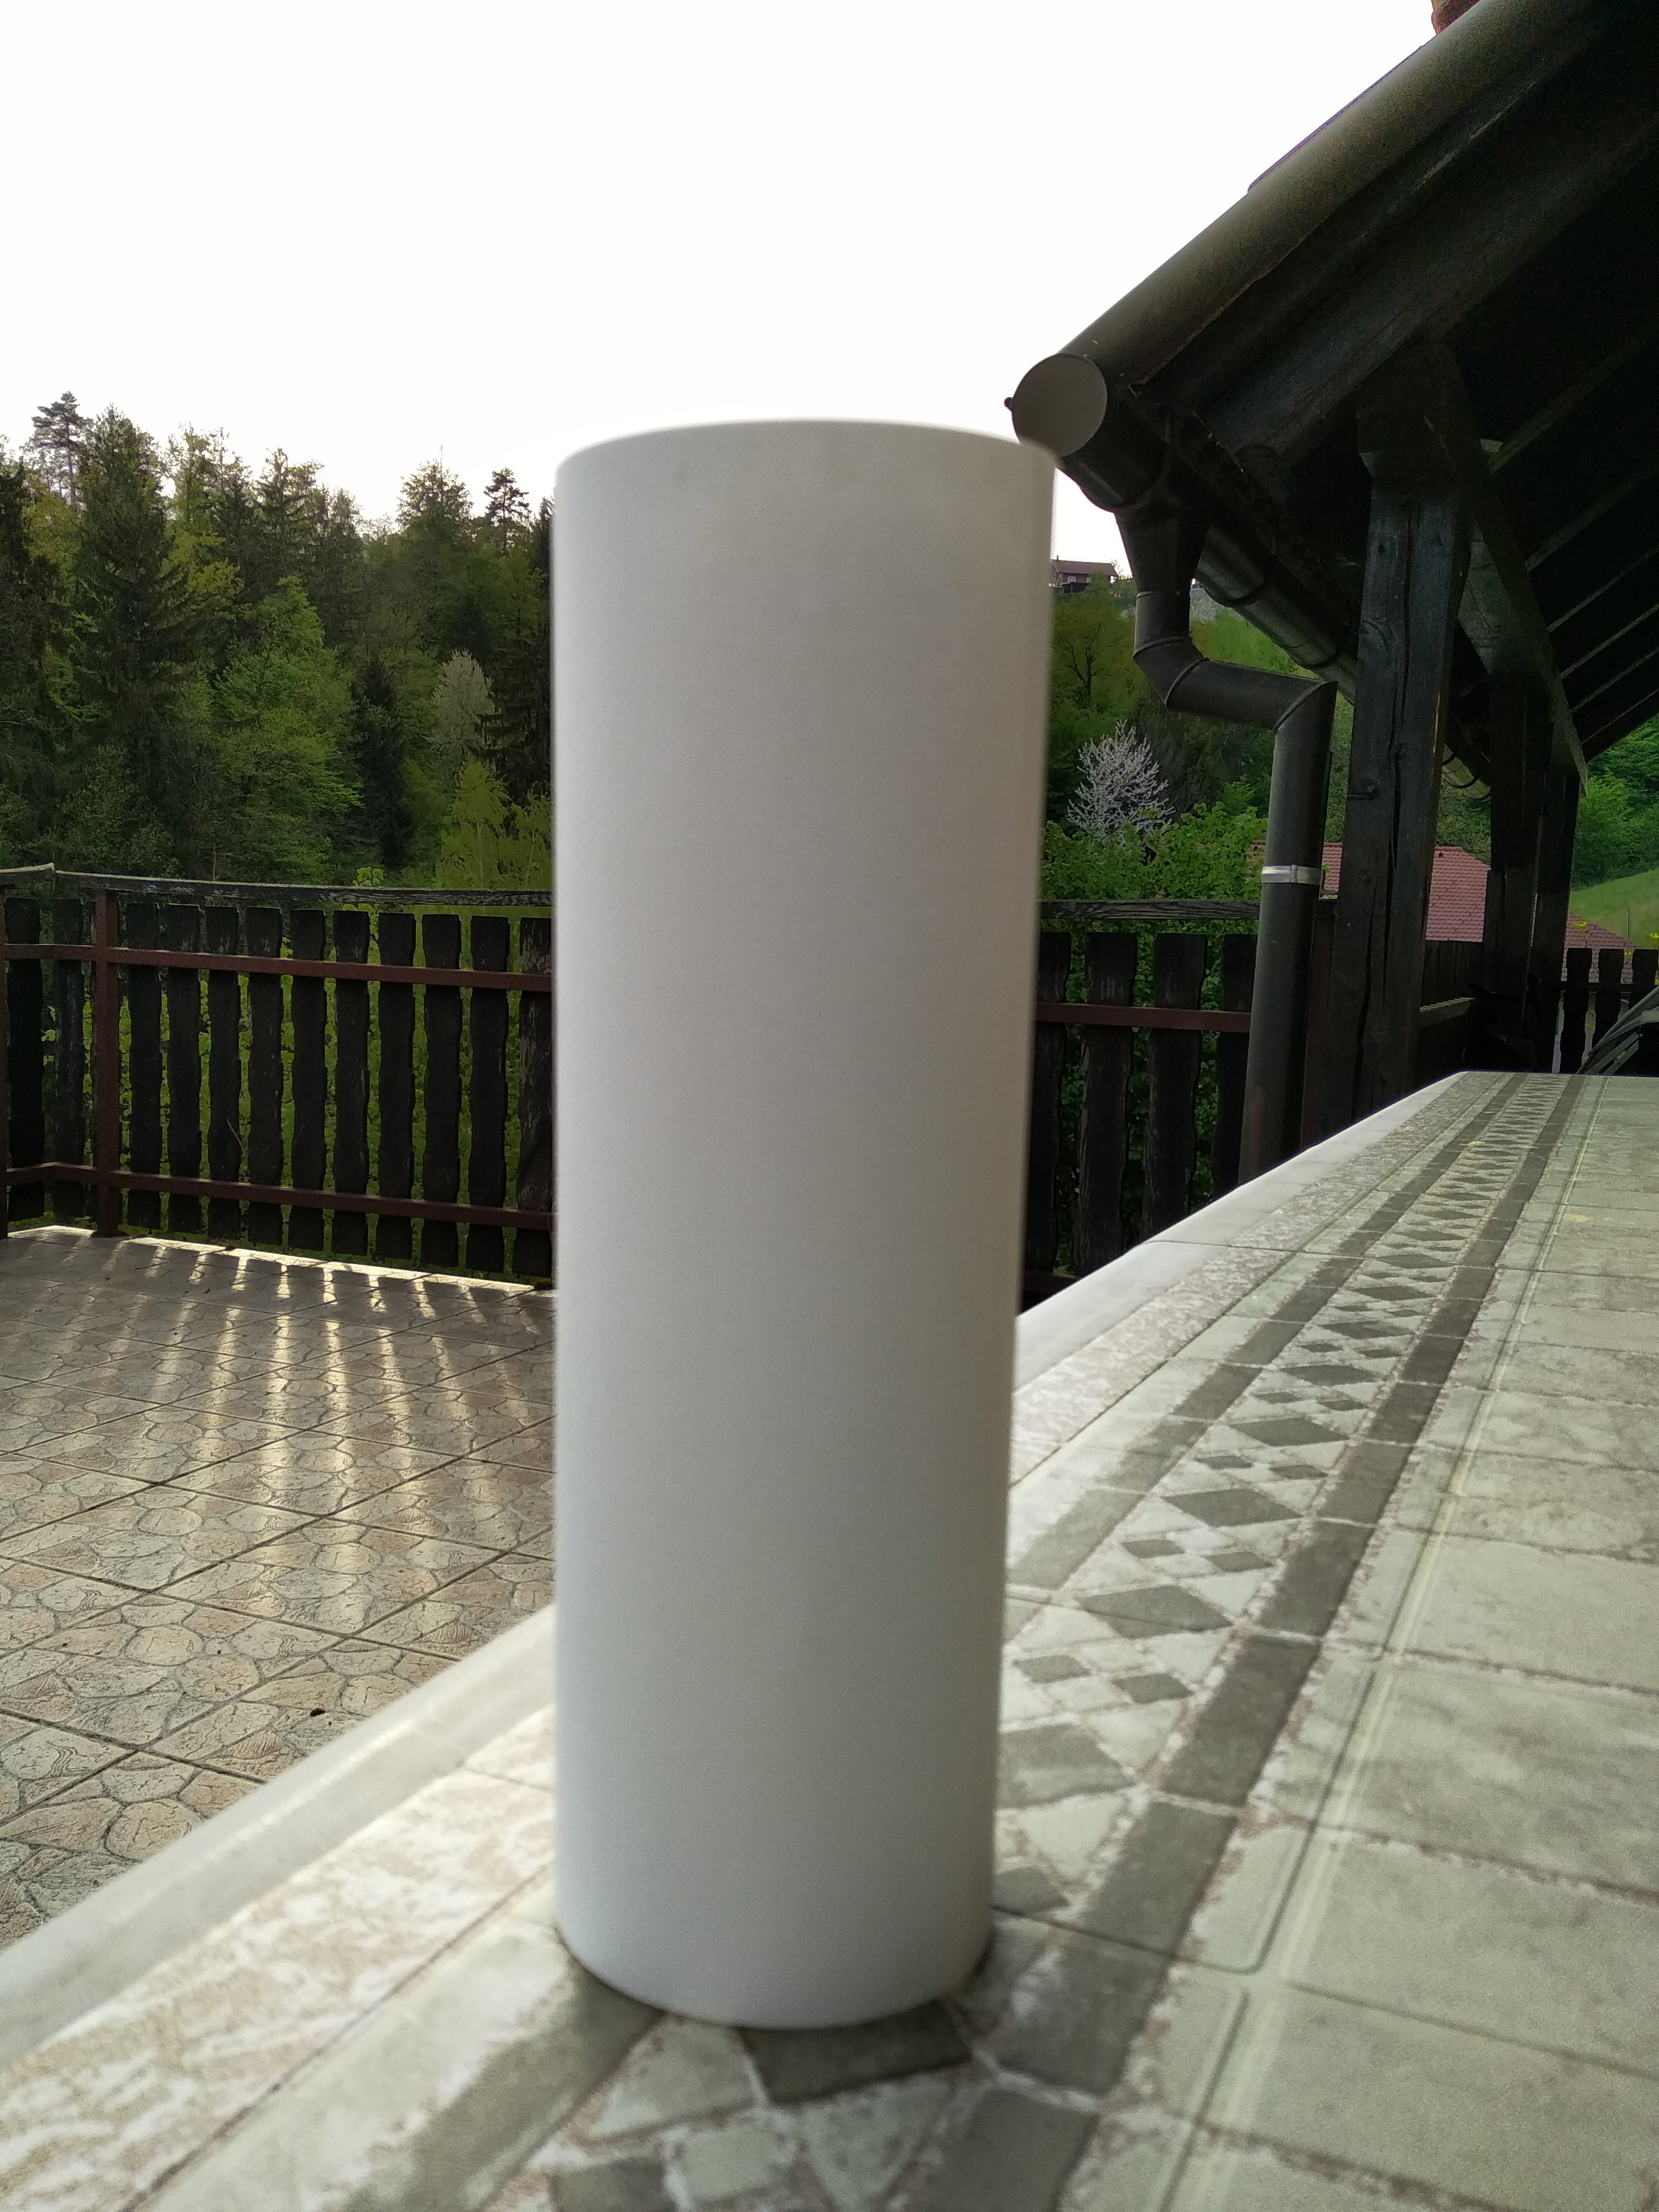
\includegraphics[width=.13\linewidth]{images/test05.jpg}
		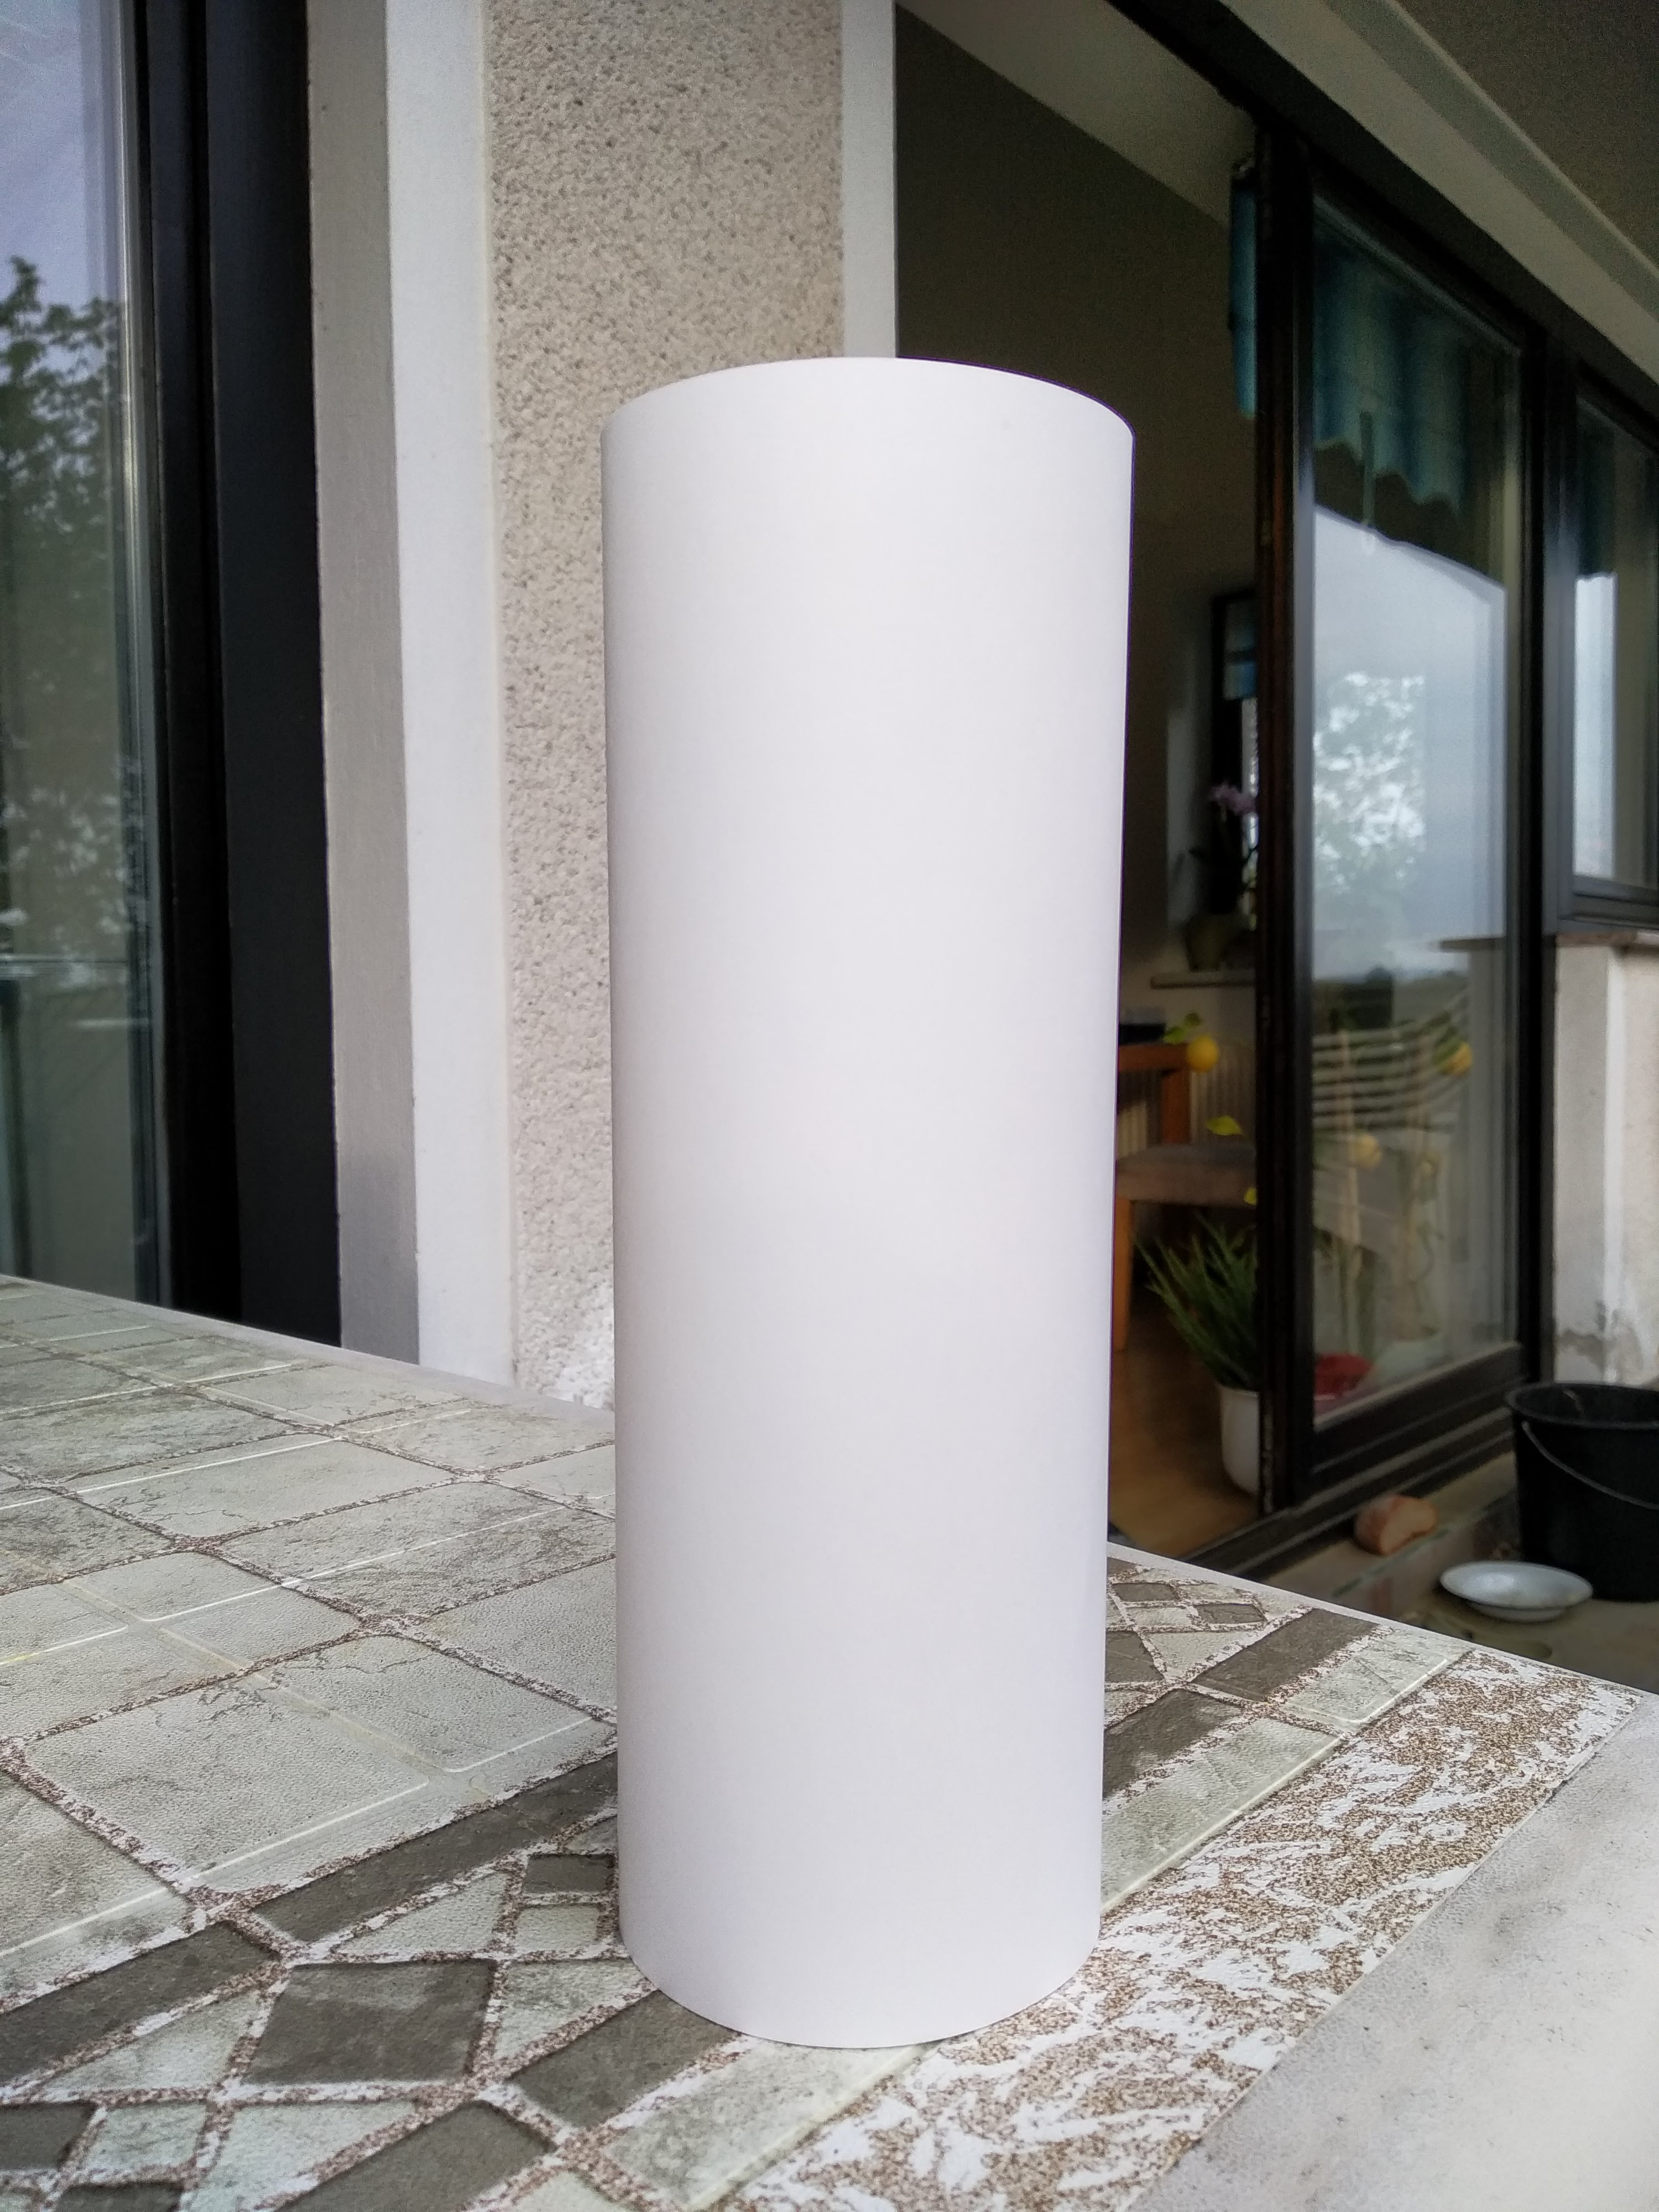
\includegraphics[width=.13\linewidth]{images/test06.jpg} \\
		\vspace{3pt}
		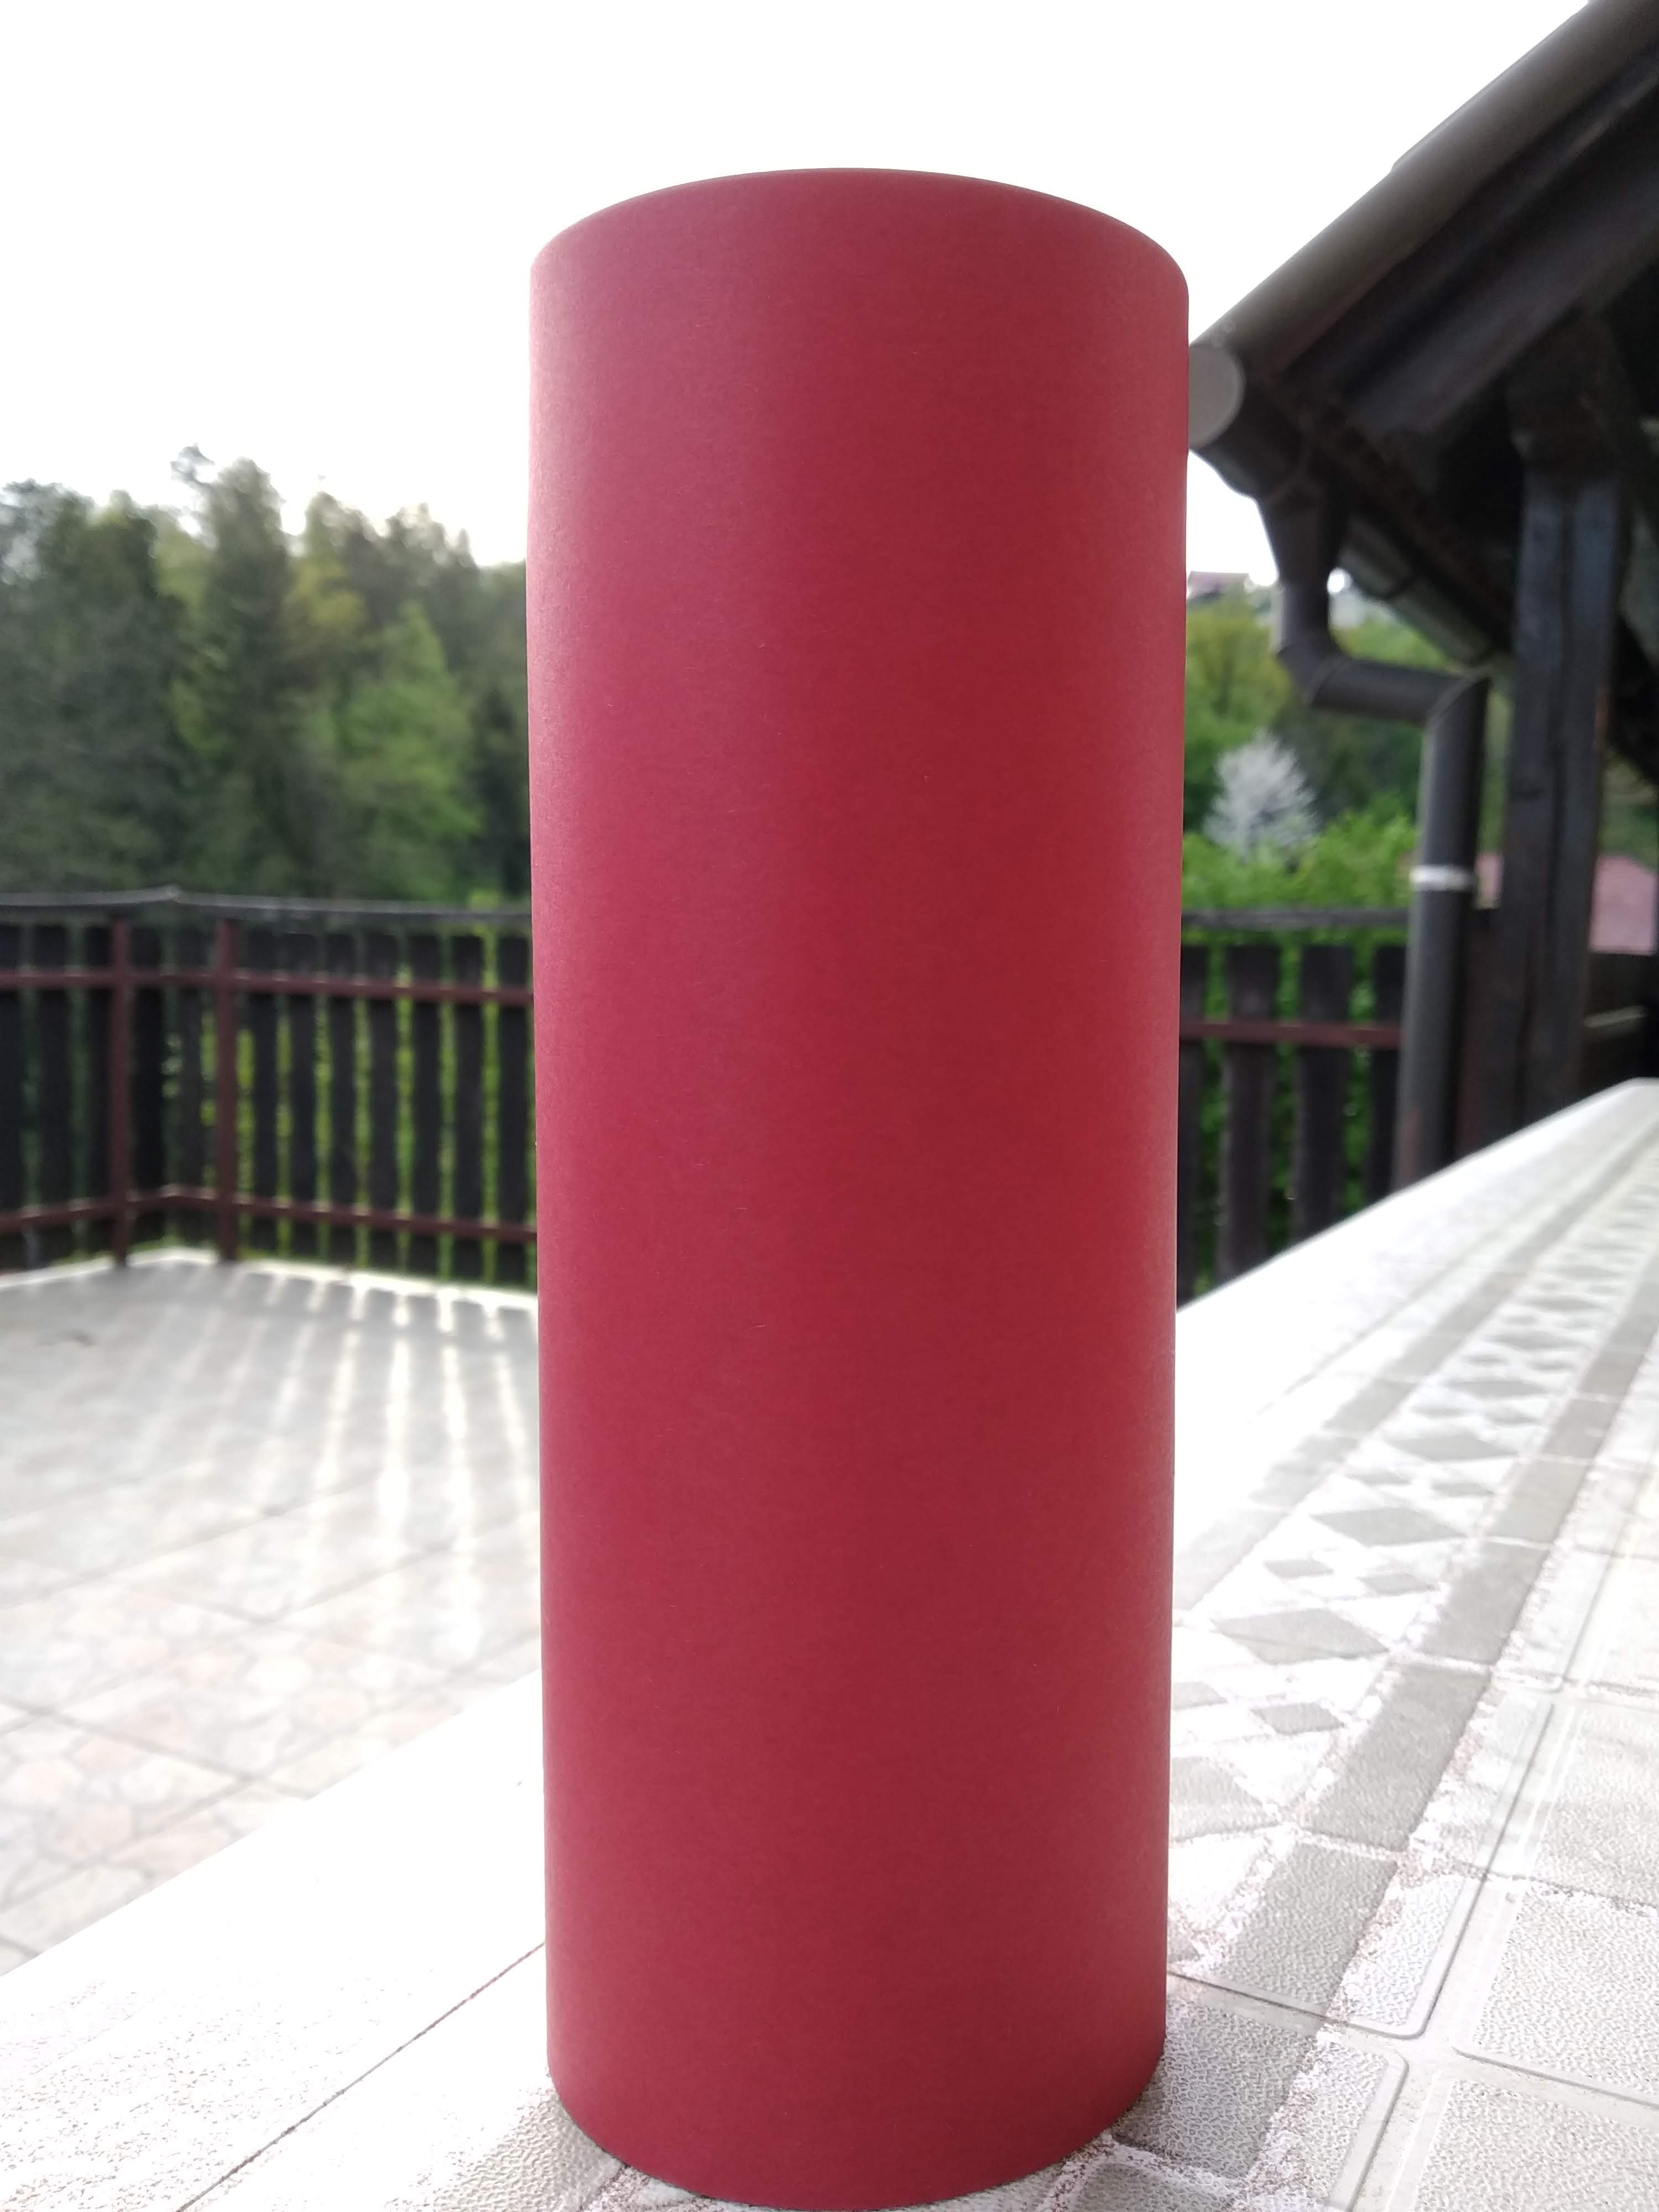
\includegraphics[width=.13\linewidth]{images/test07.jpg}
		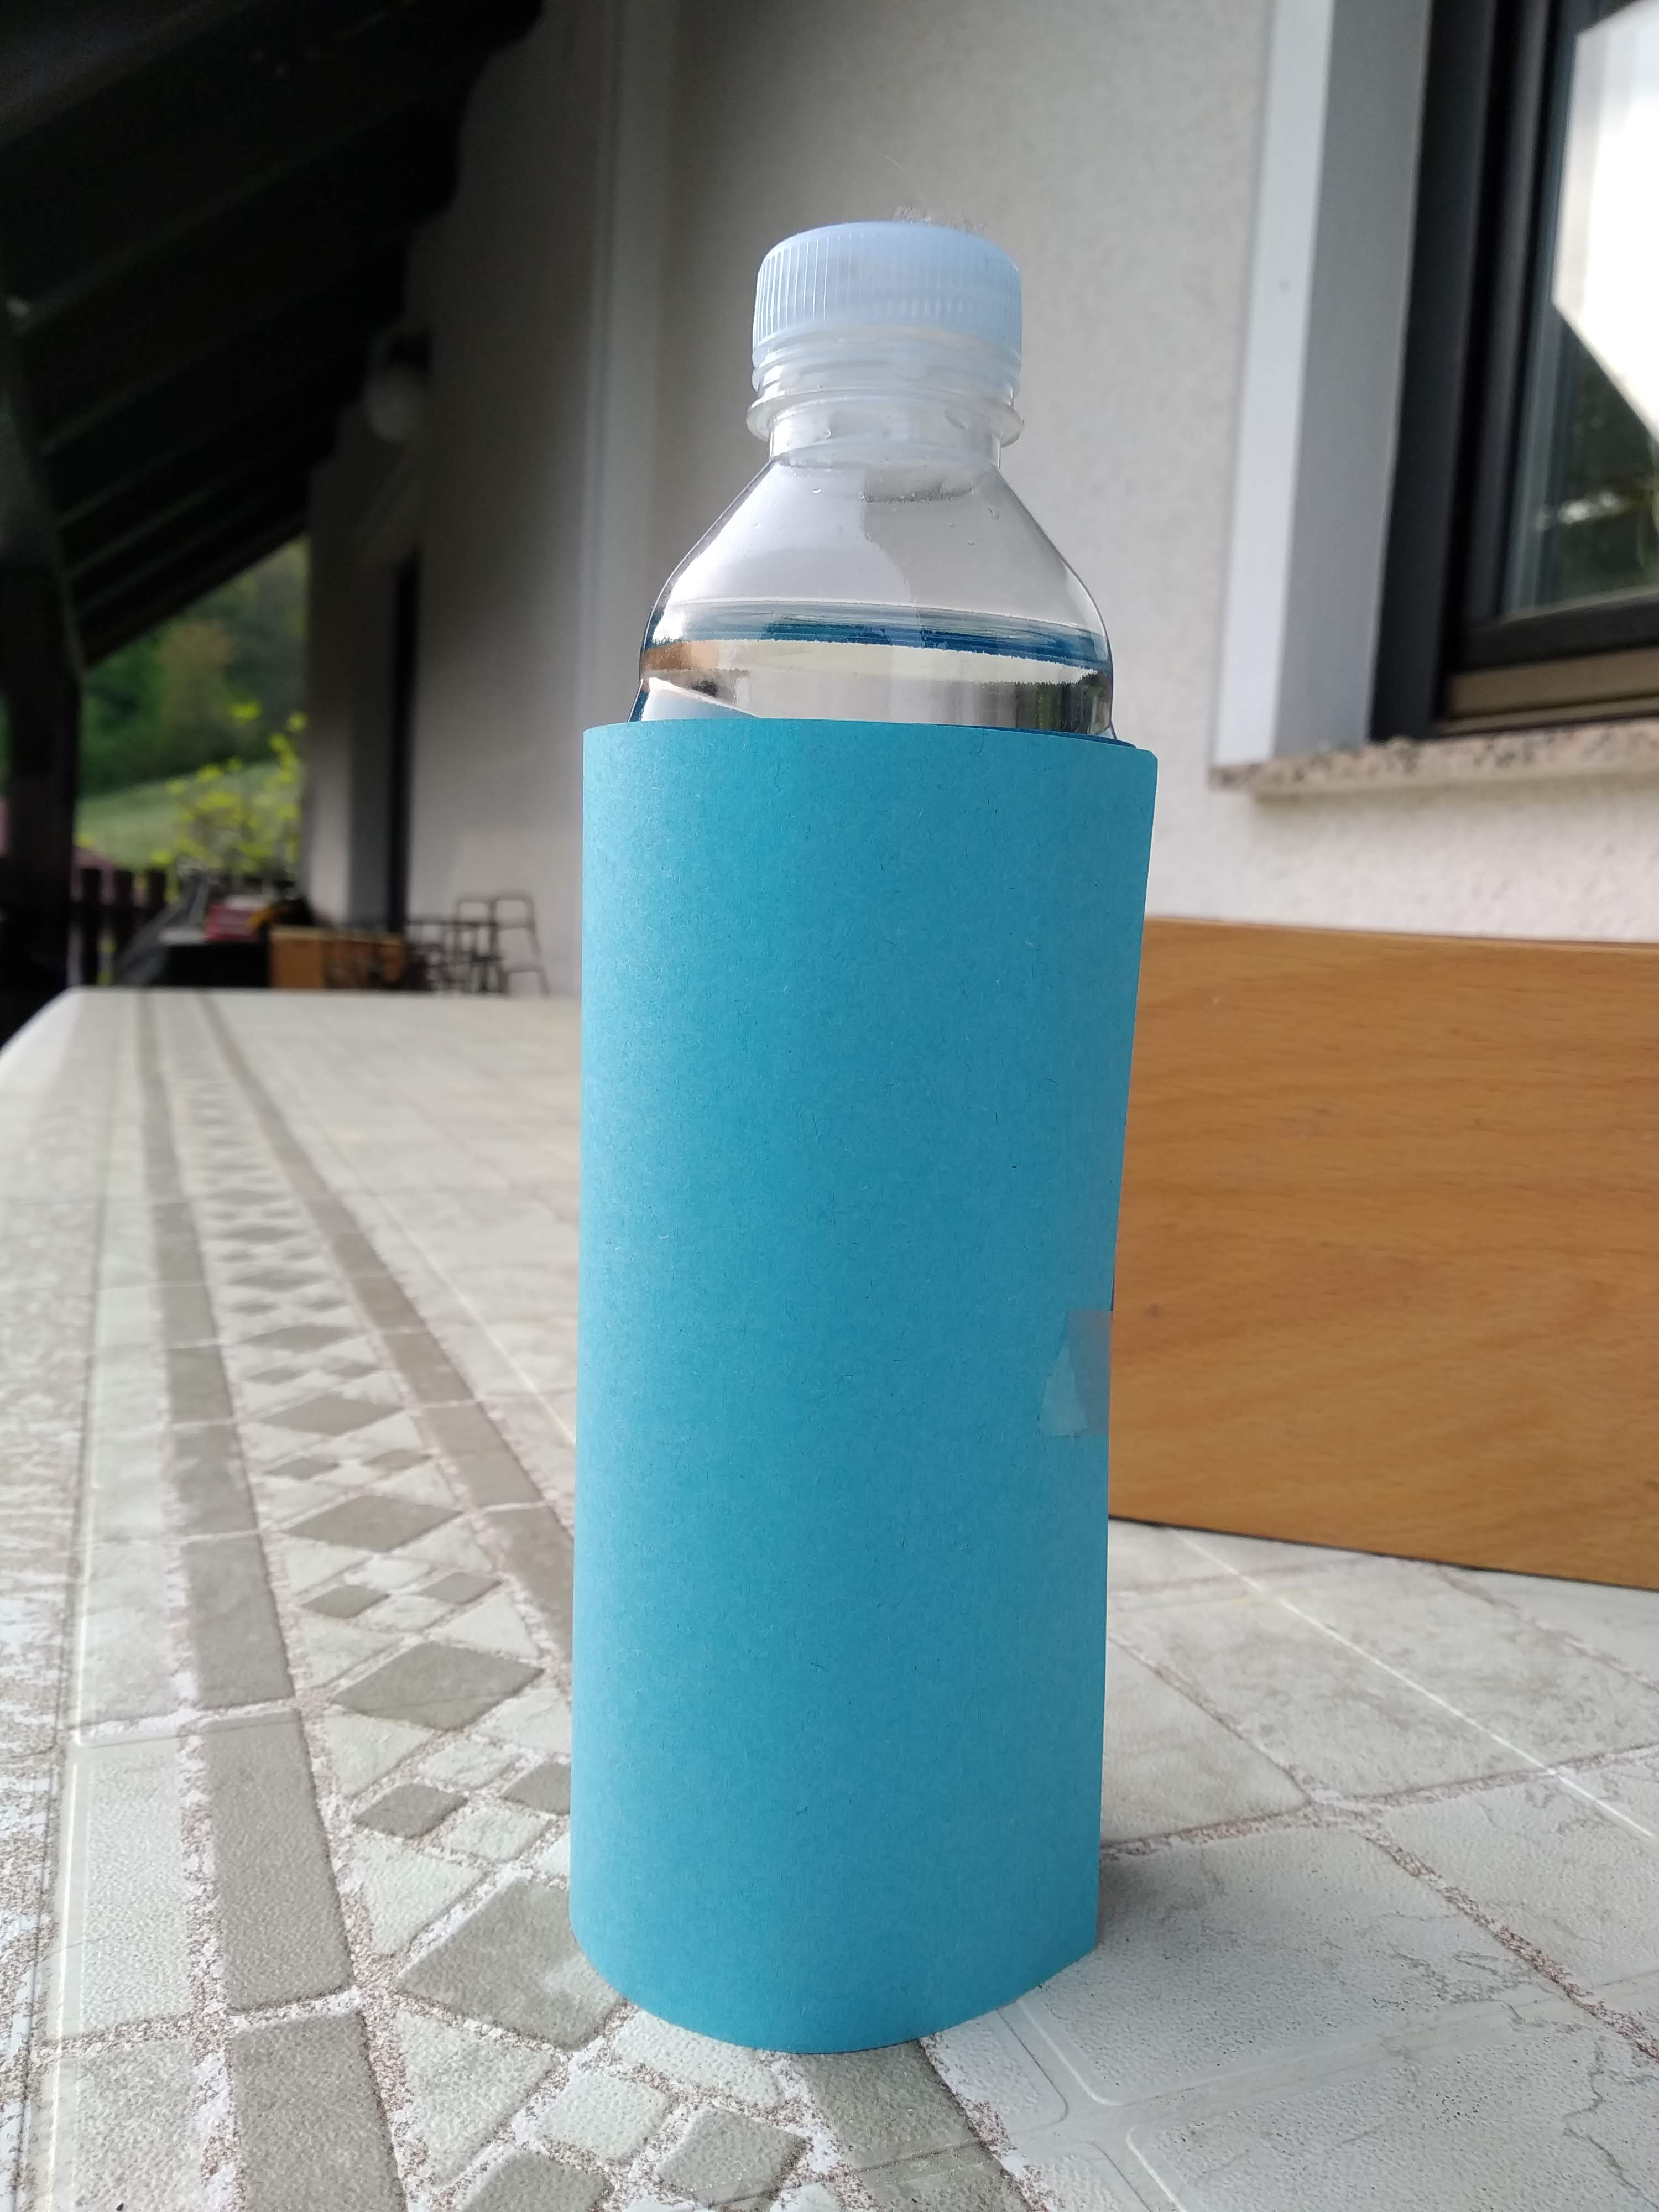
\includegraphics[width=.13\linewidth]{images/test08.jpg}
		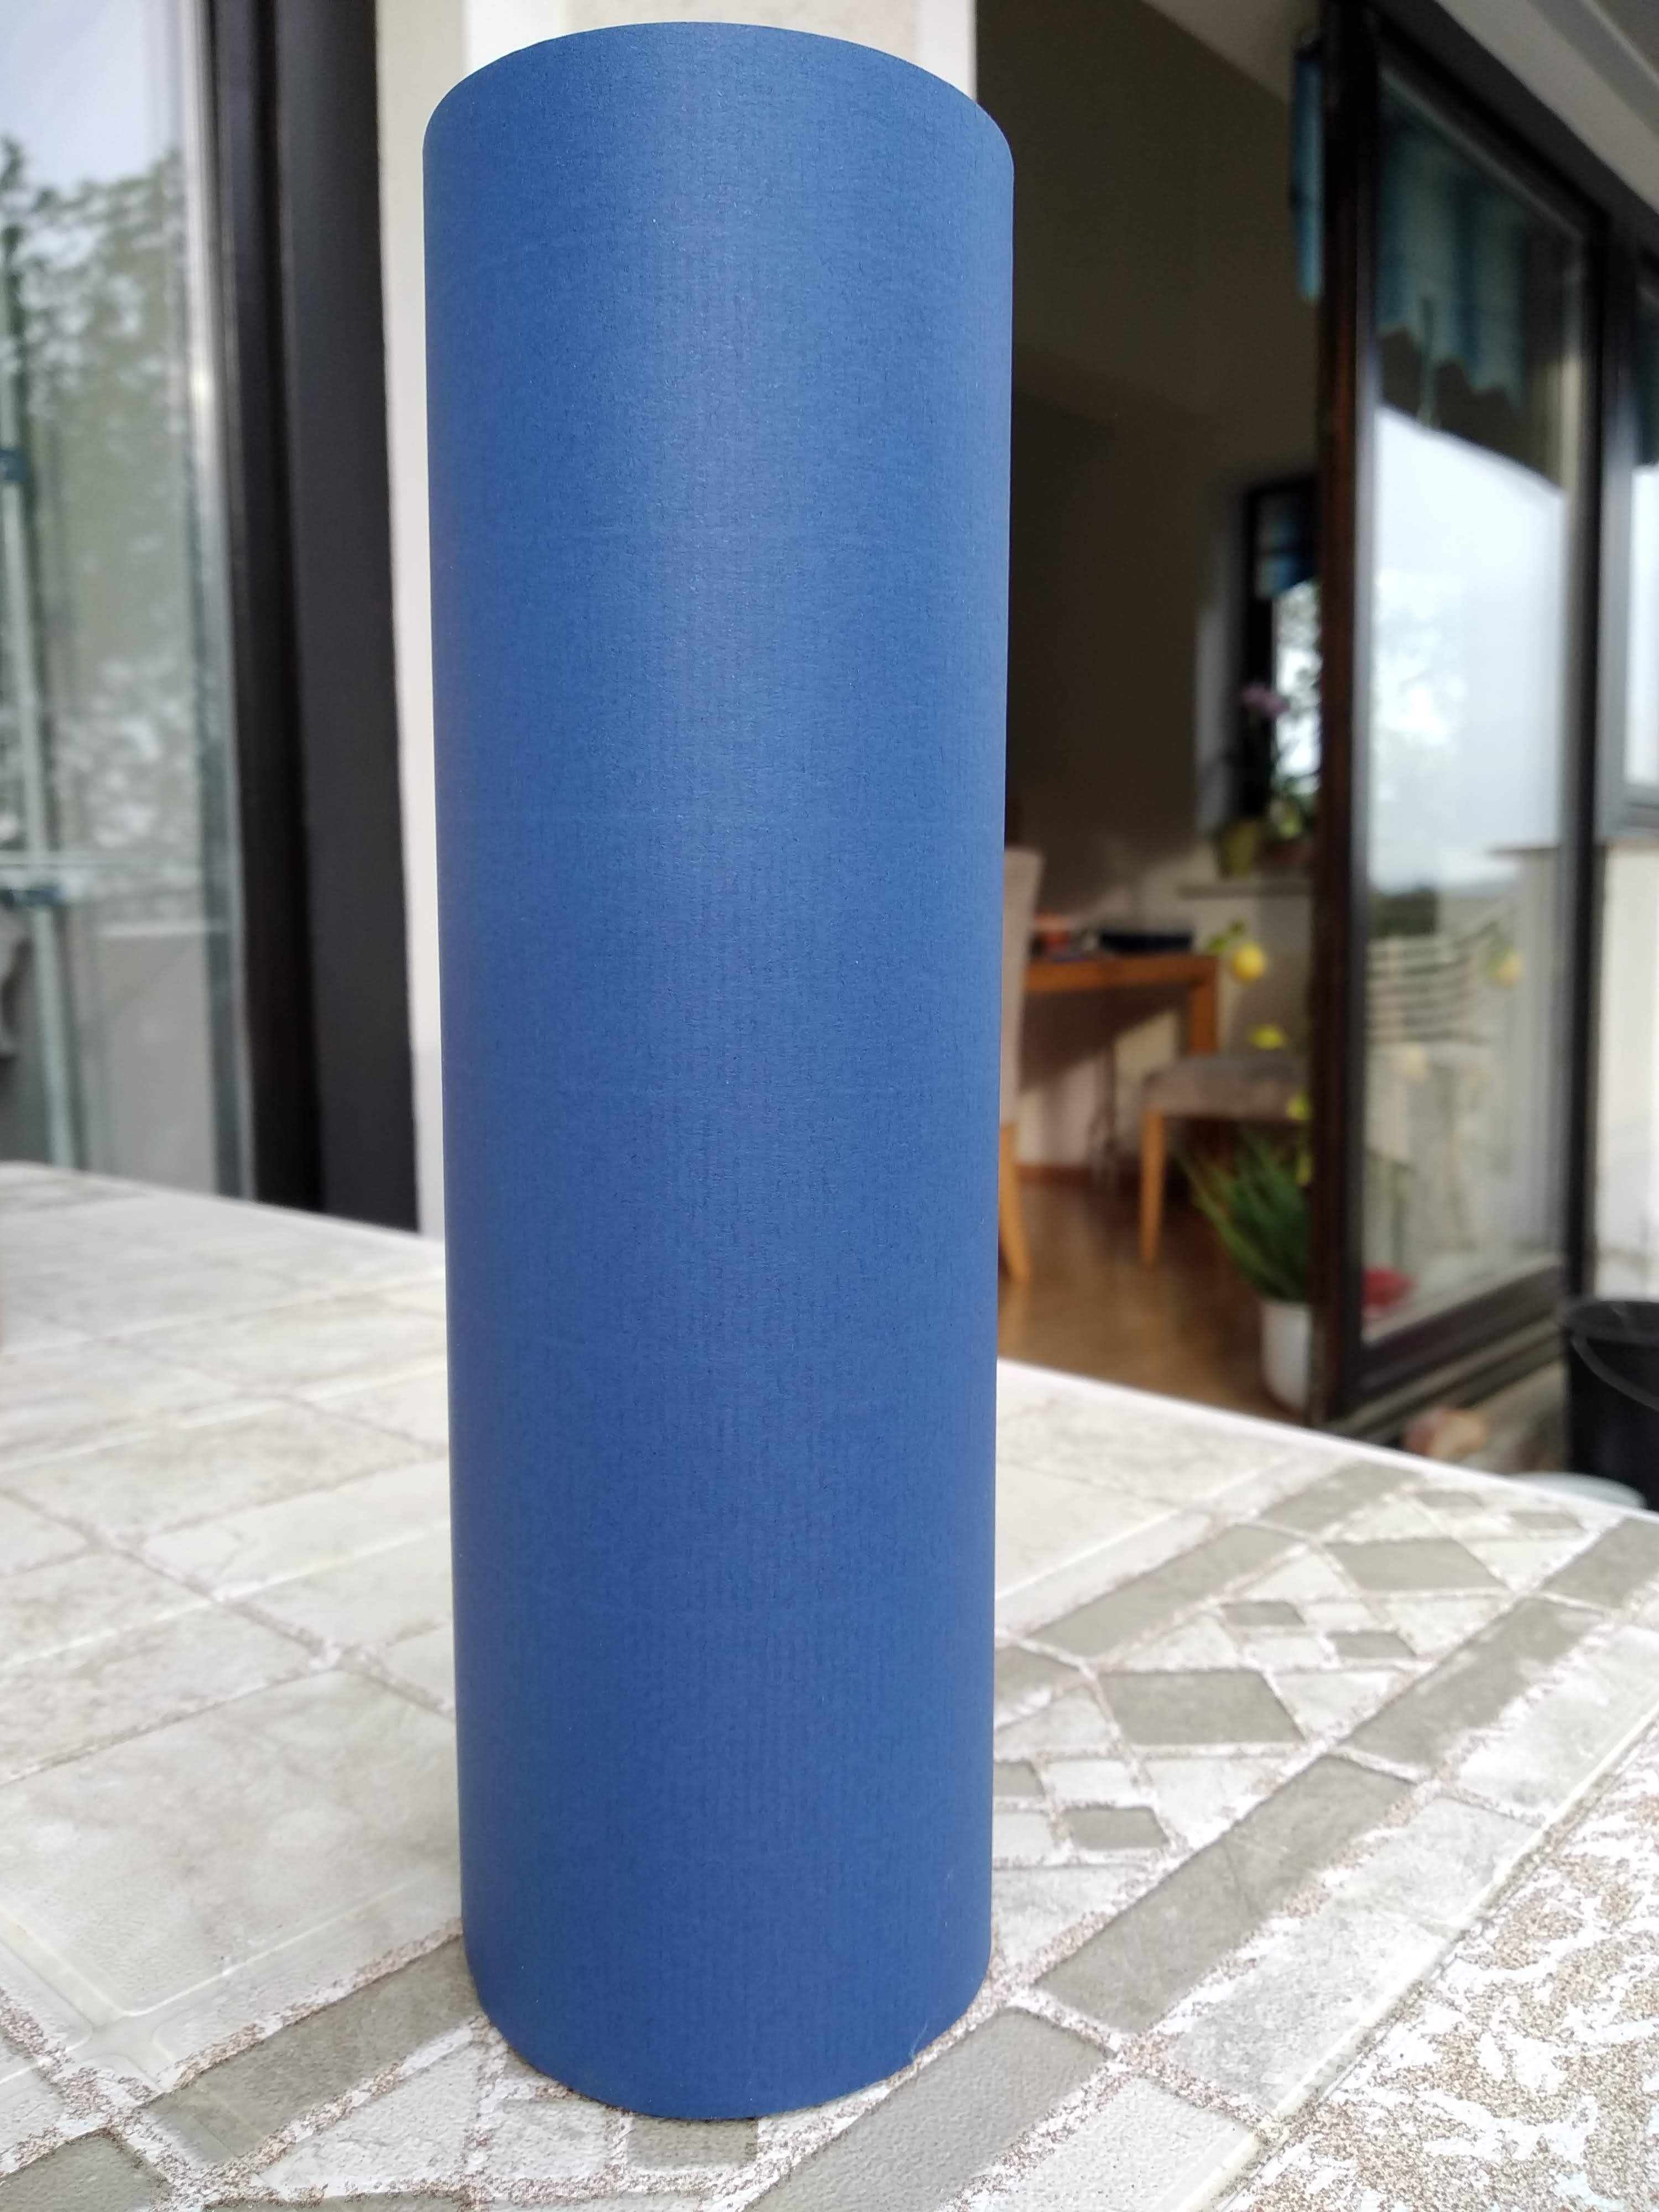
\includegraphics[width=.13\linewidth]{images/test_09_remove_if_too_many_photos.jpg}
		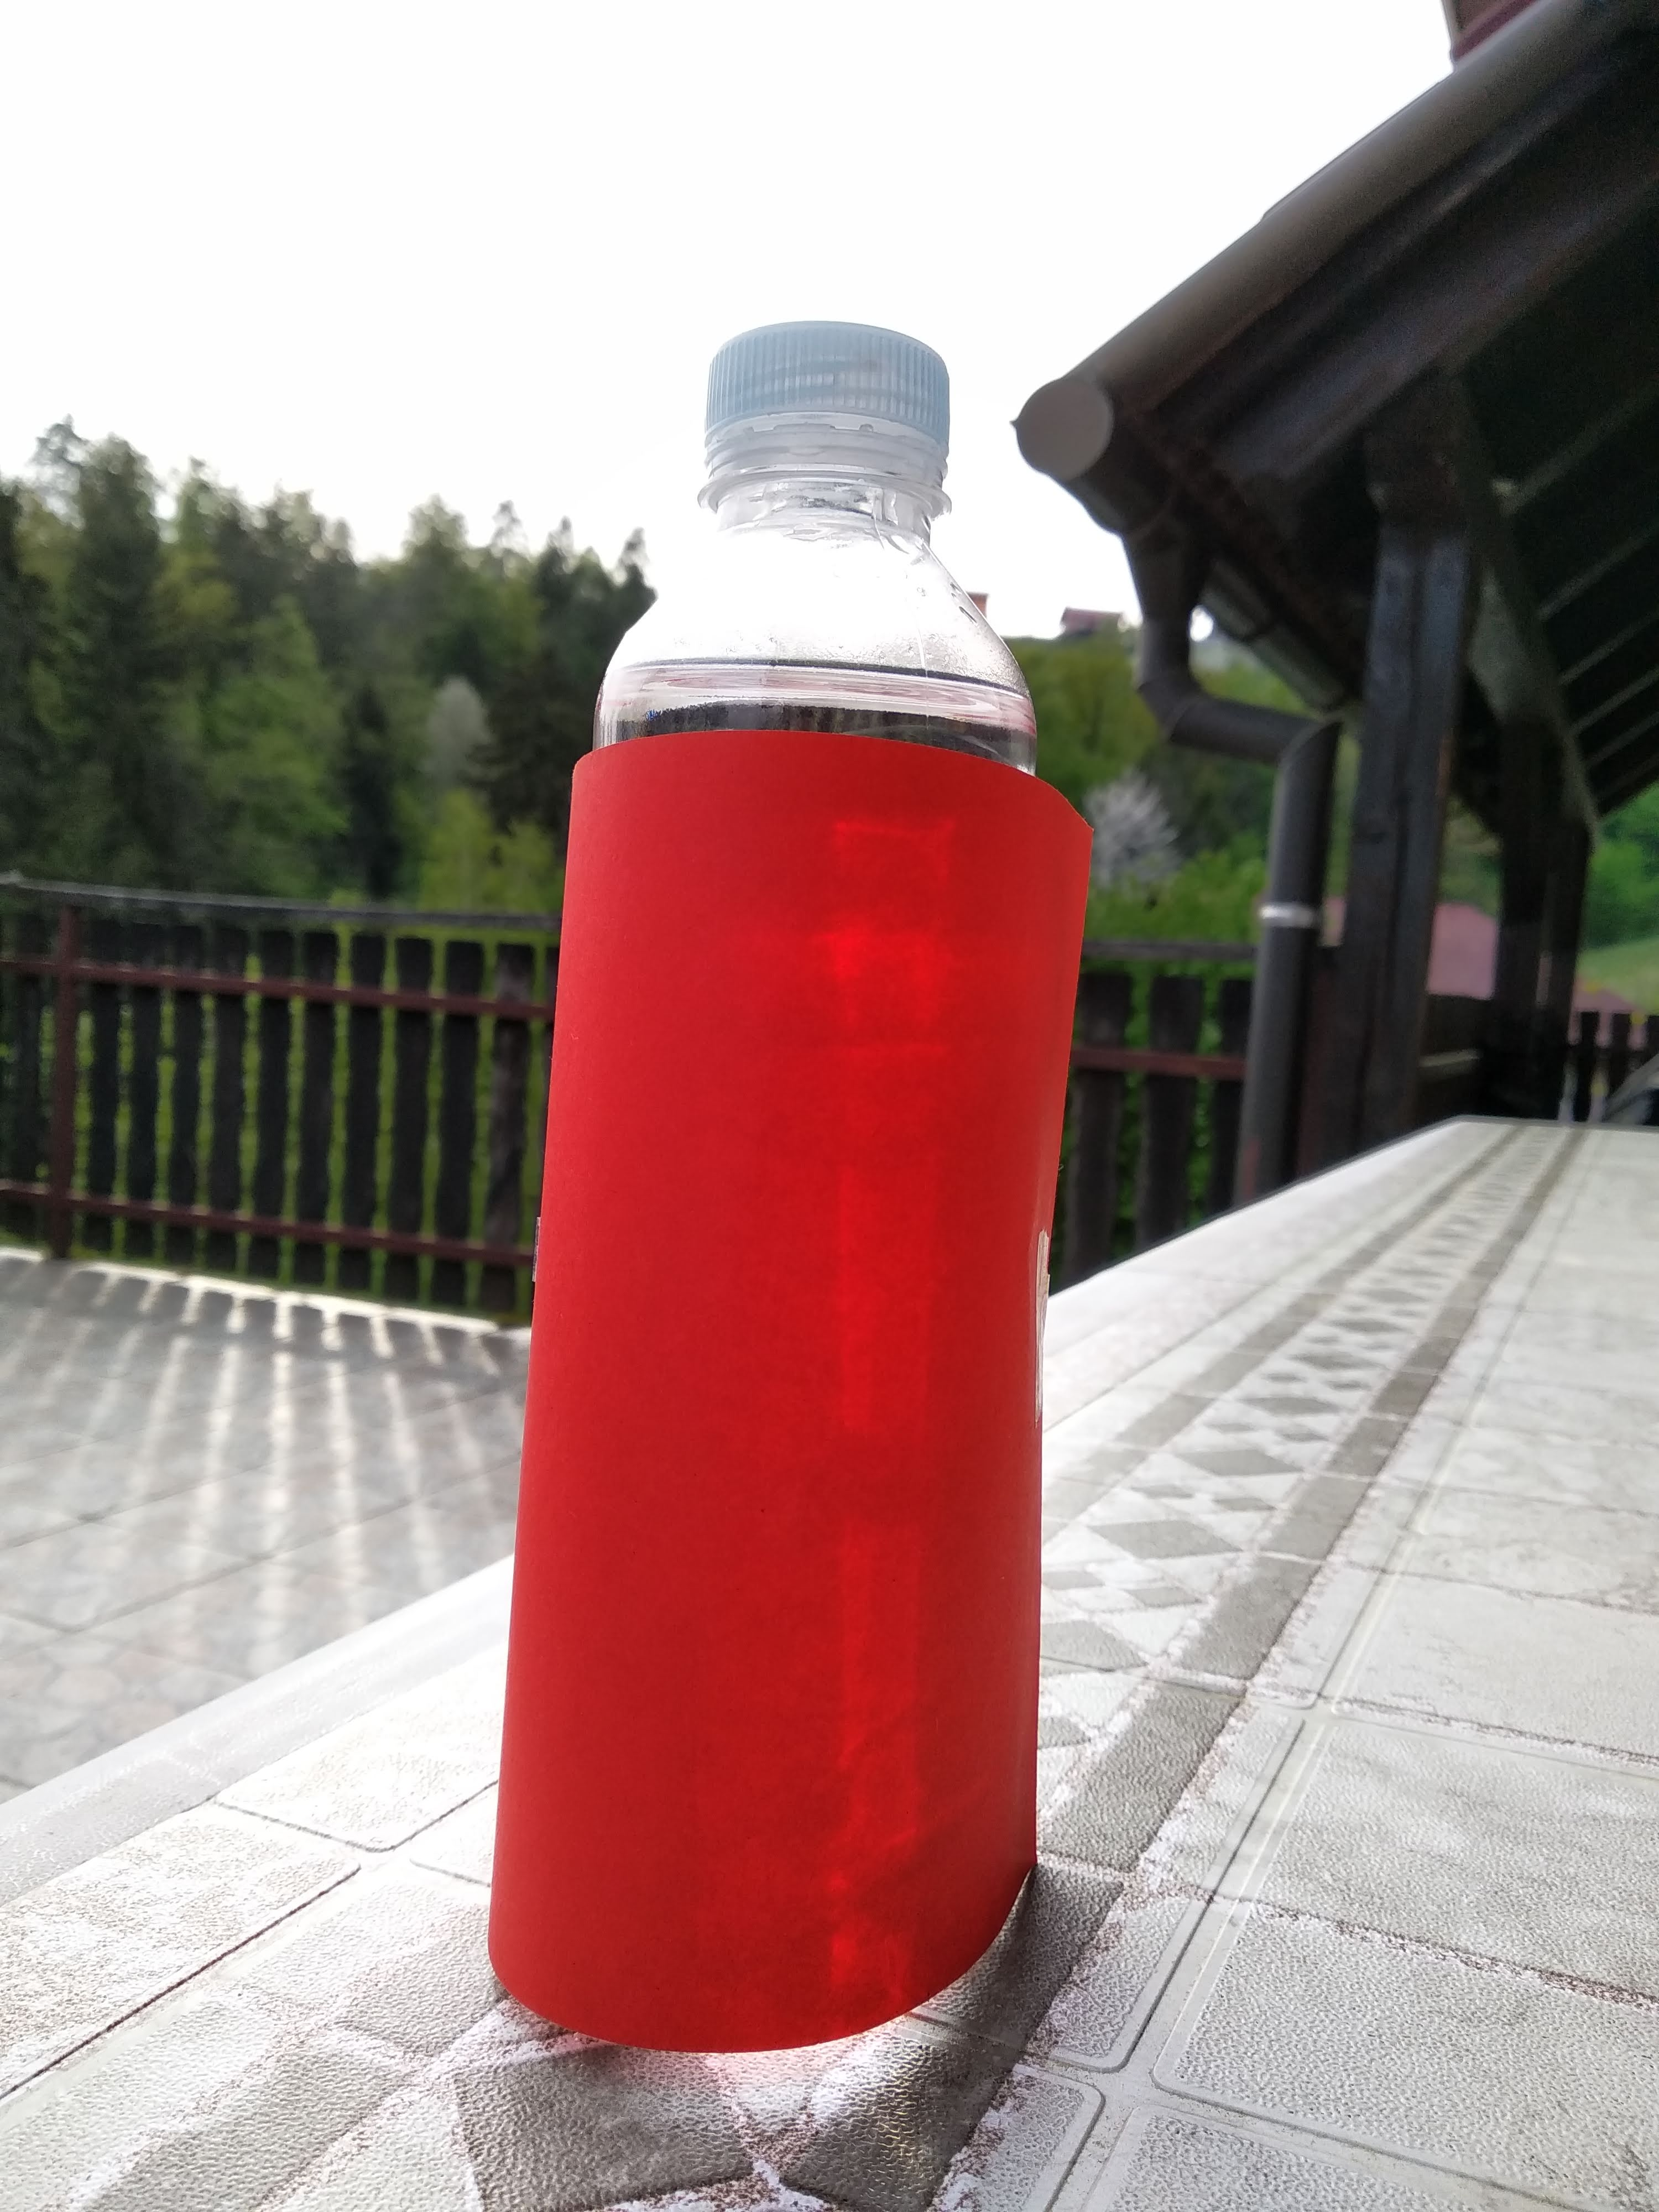
\includegraphics[width=.13\linewidth]{images/test_10_remove_if_too_many_photos.jpg}
		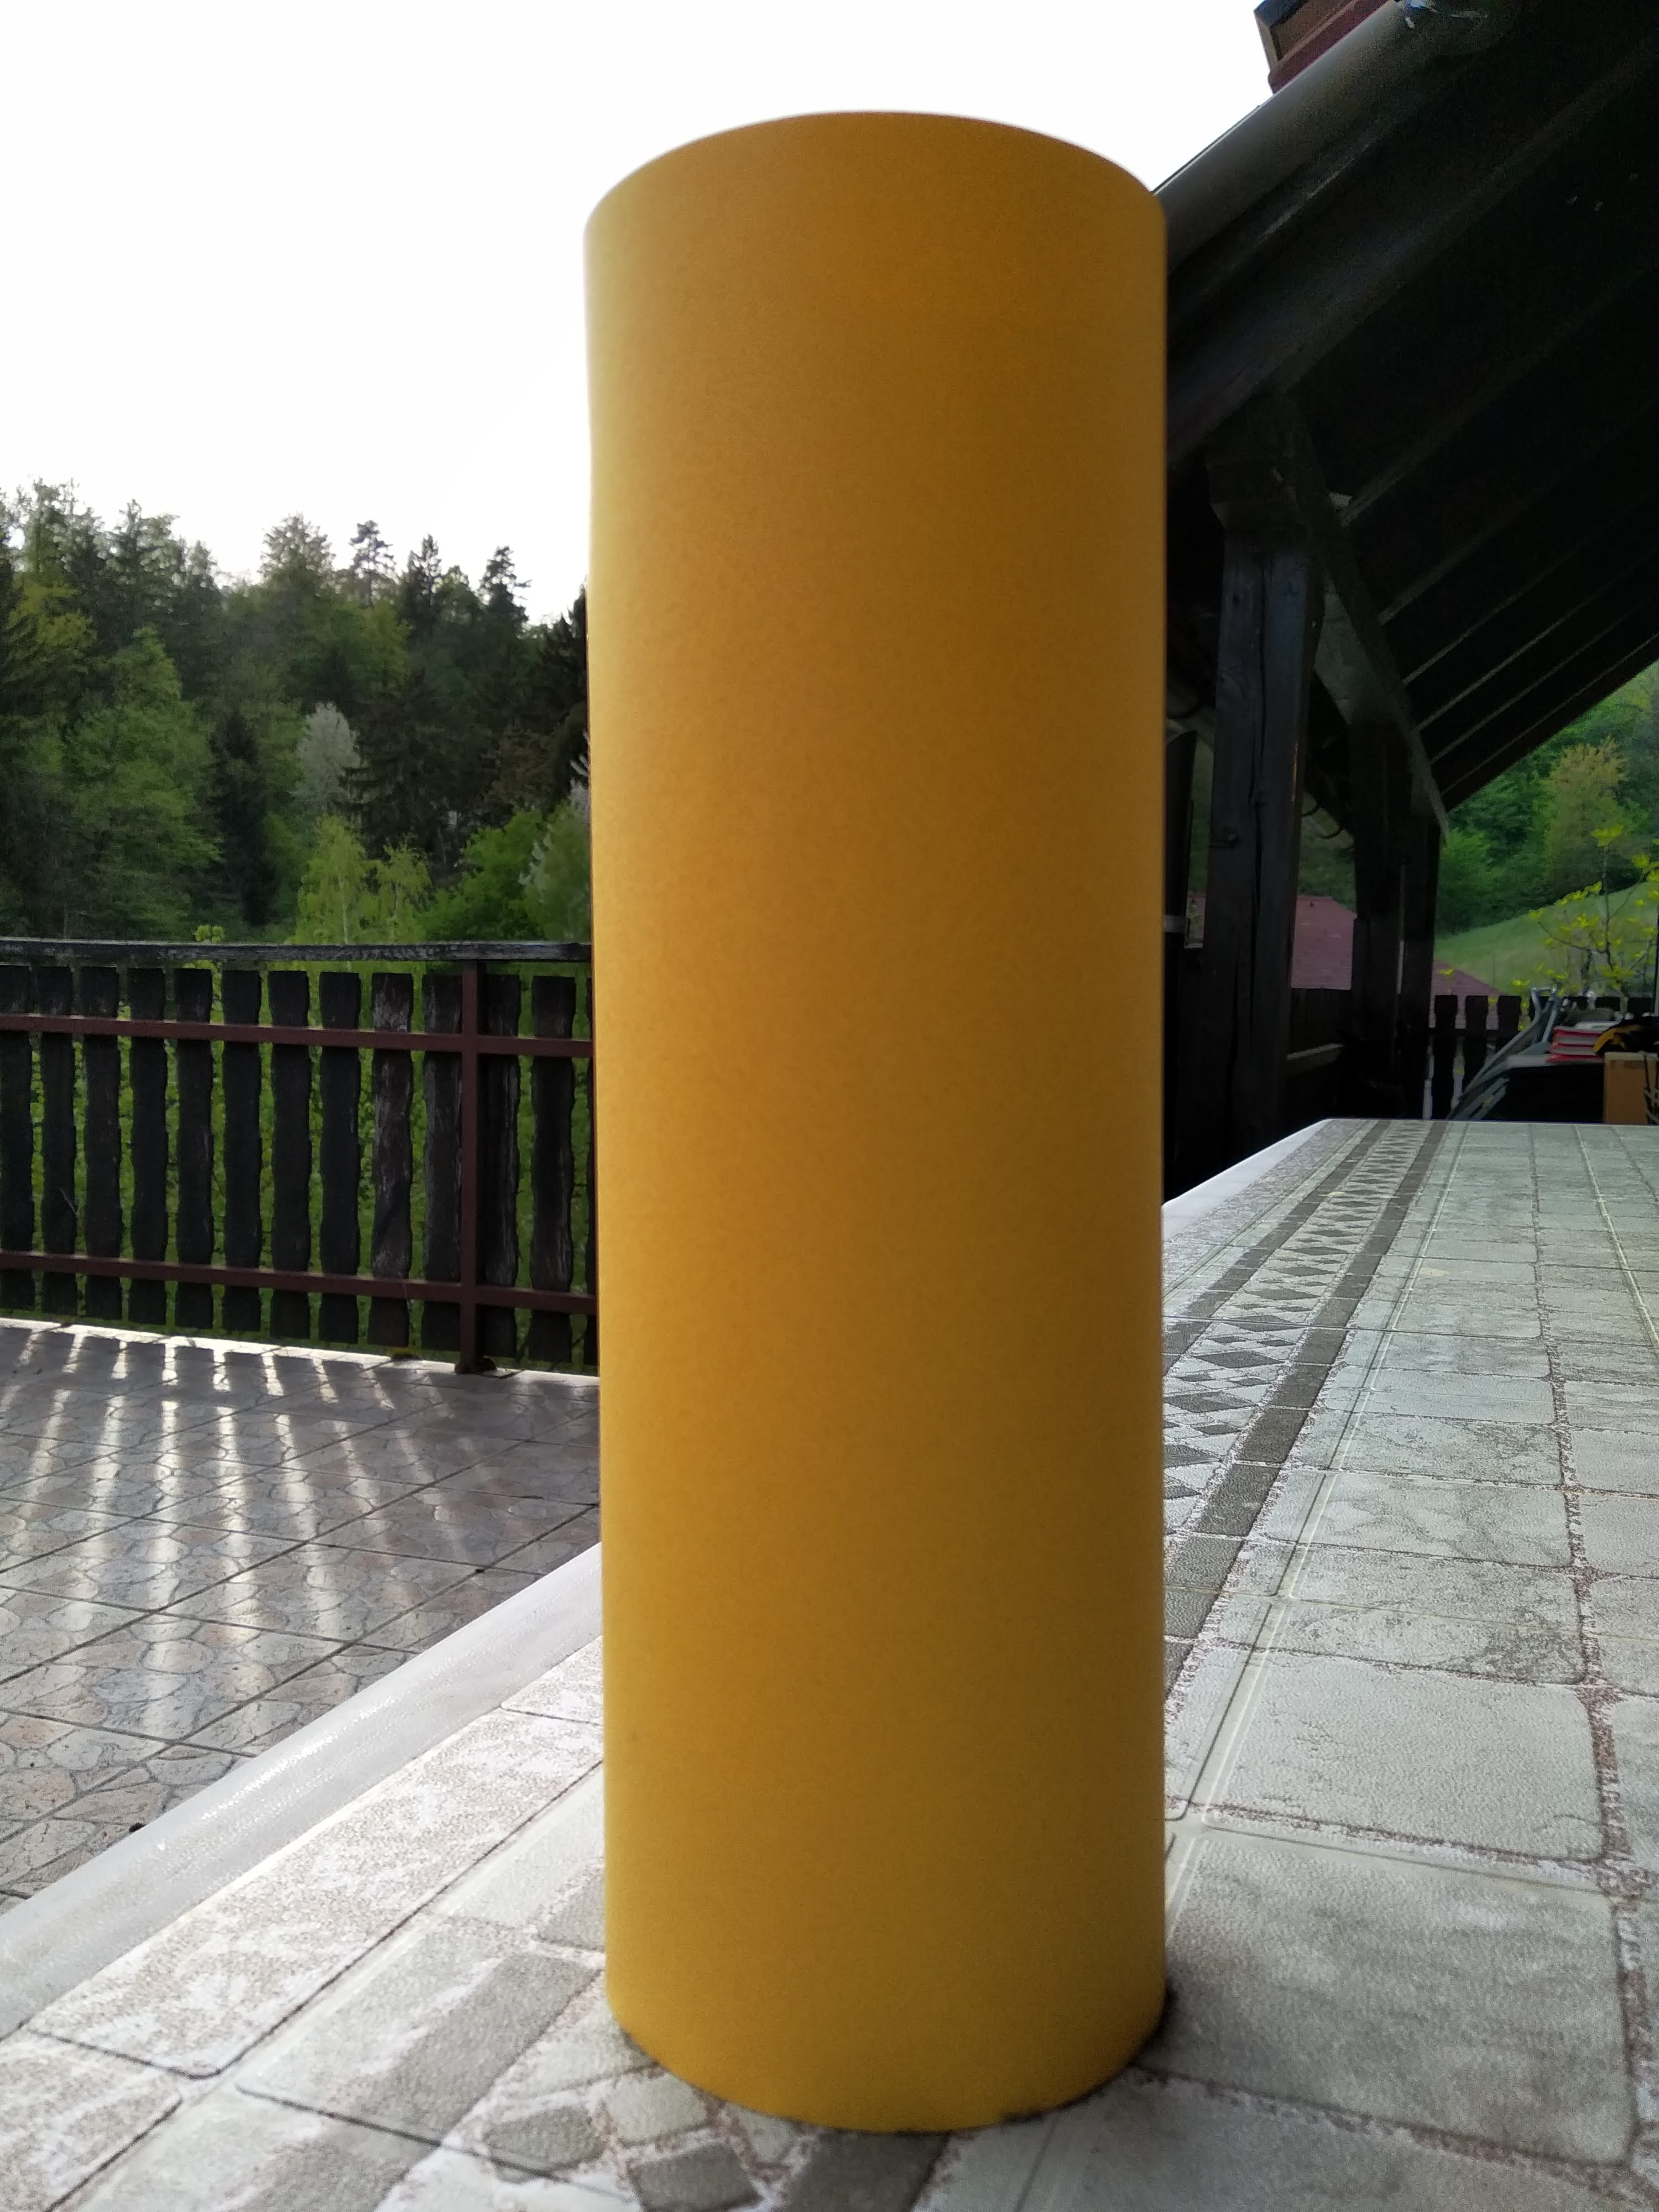
\includegraphics[width=.13\linewidth]{images/test_11_remove_if_too_many_photos.jpg}
		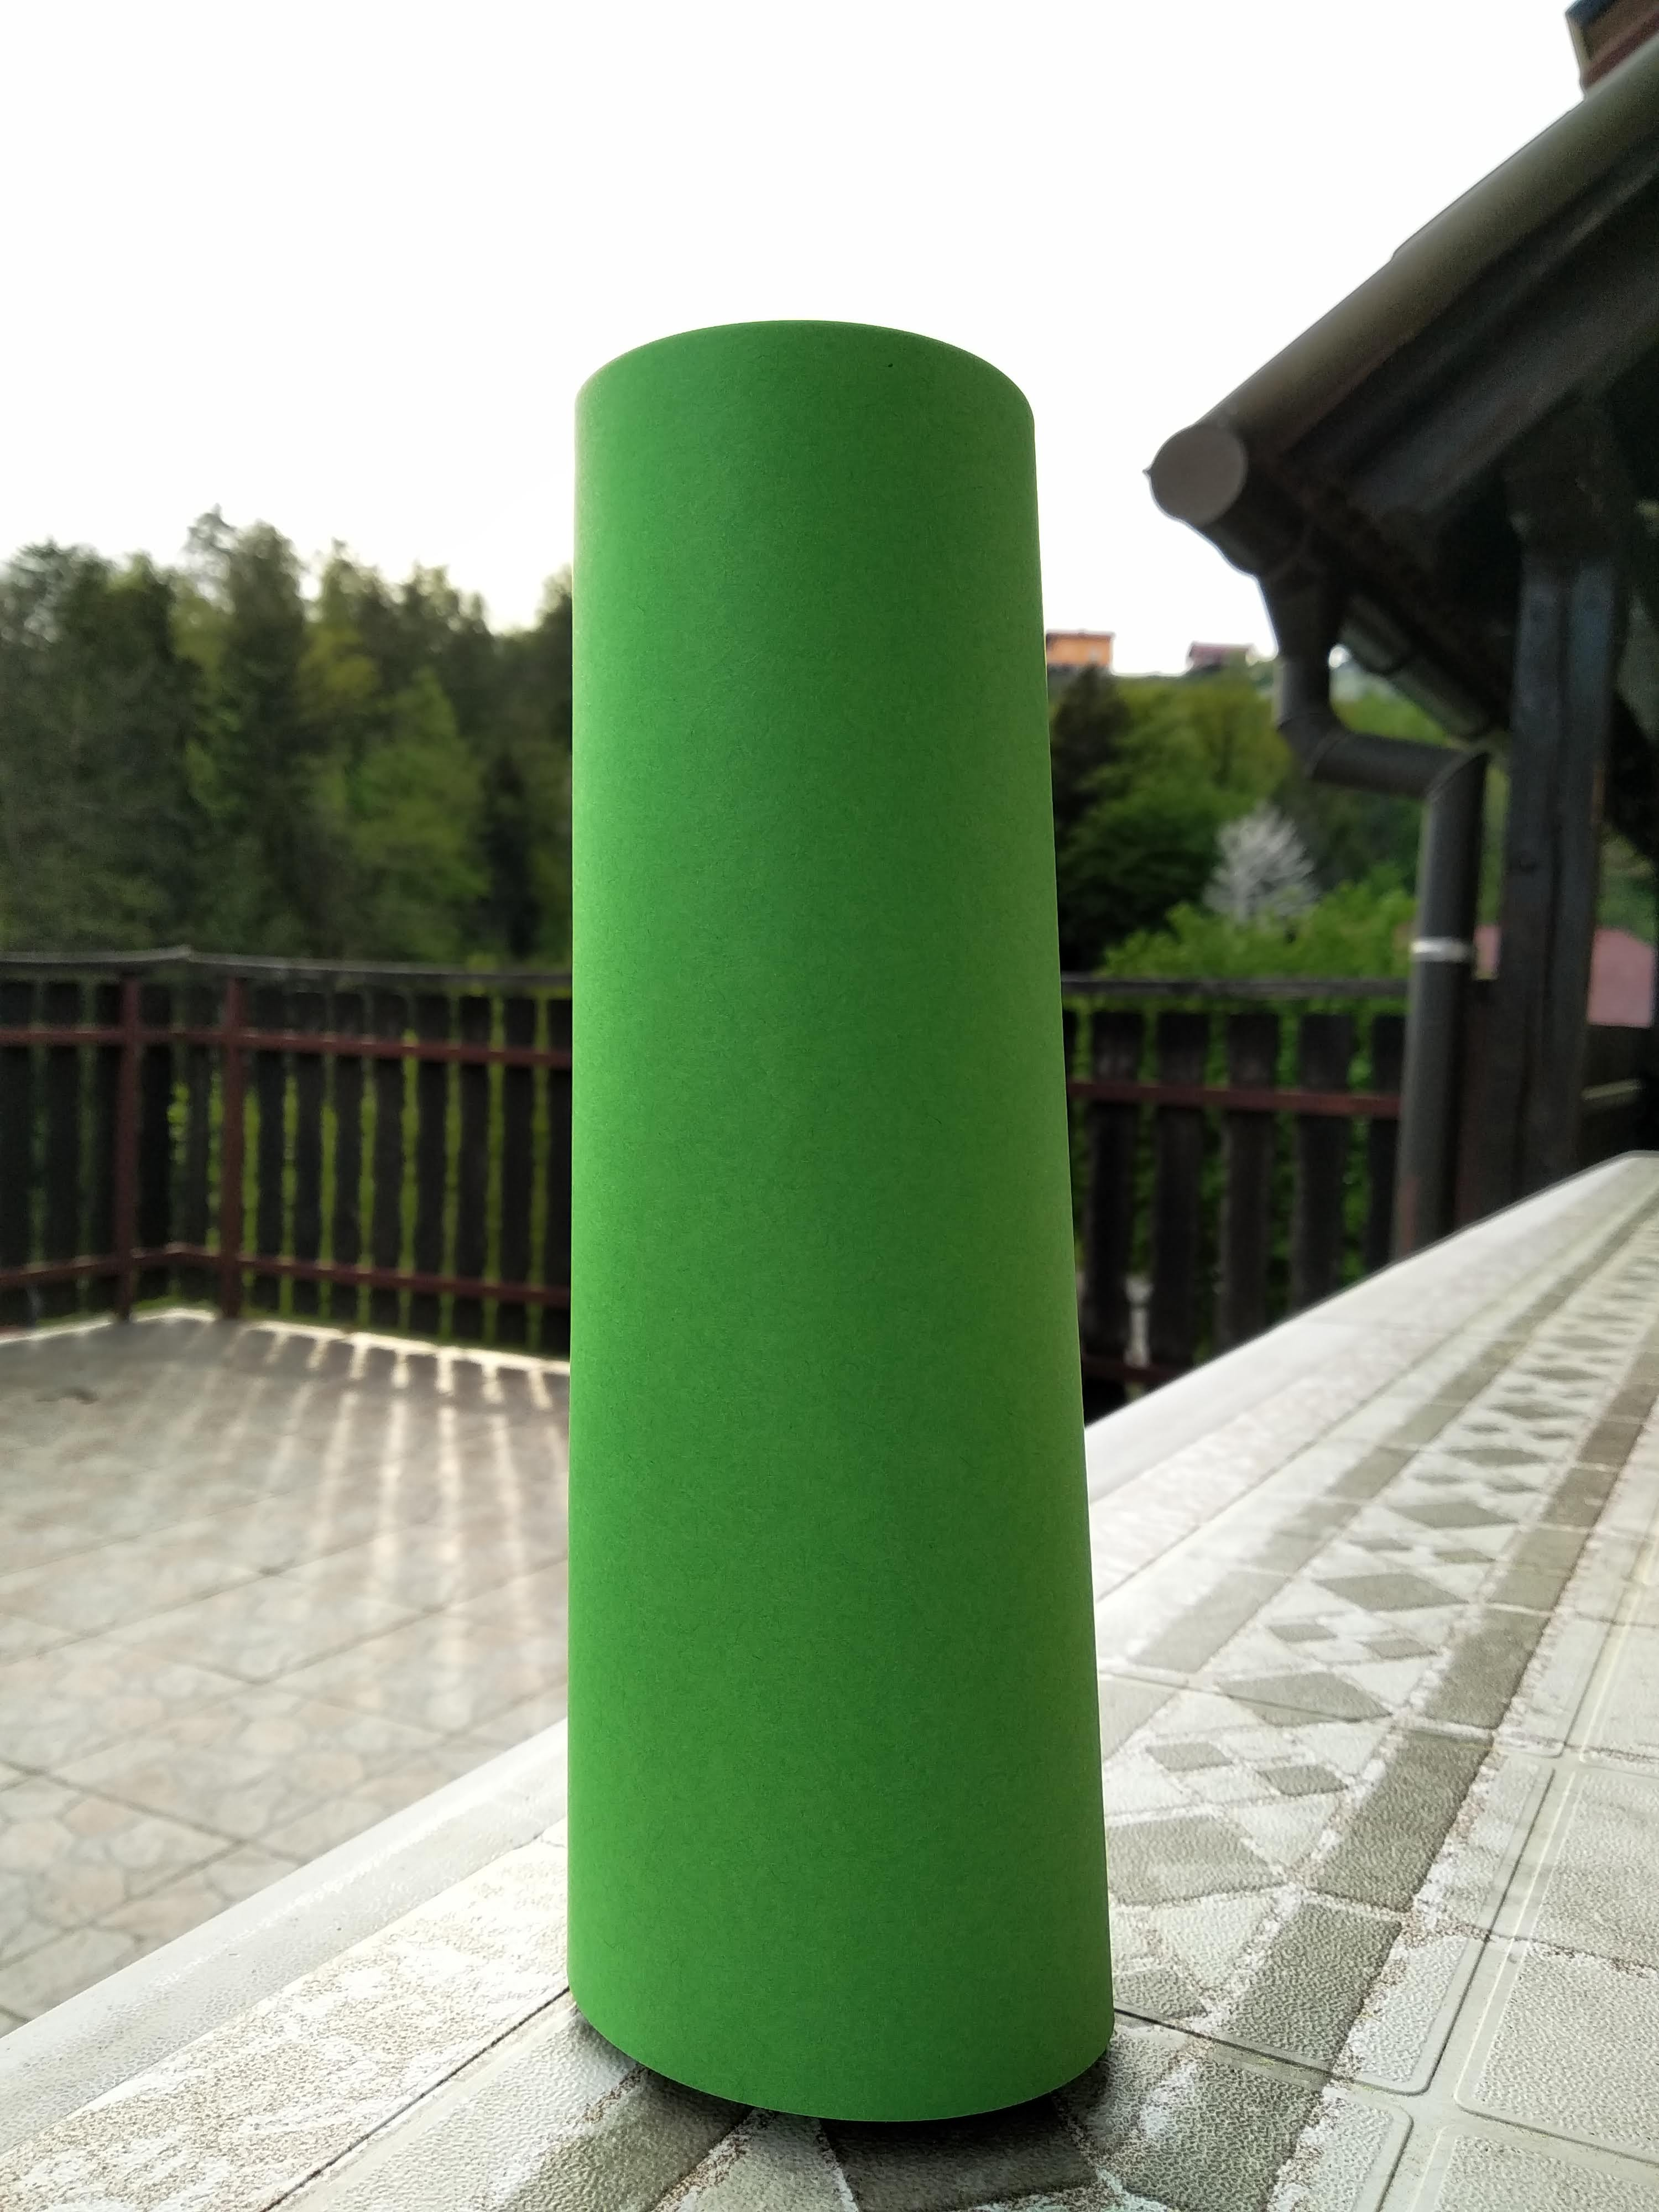
\includegraphics[width=.13\linewidth]{images/test_12_remove_if_too_many_photos.jpg}
		\caption{Second set of photos}
	\end{figure}

	\subsection{Preprocessing photos}

	To prepare the images for classifiers, we cropped the circles to perfect circles and cylinders to rectangles. Some examples of cropped cylinders are shown below.

	\begin{figure}[H]
		\centering
		
\includegraphics[width=.08\linewidth, height=.08\linewidth]{images/test_cut_01.jpg}
		
\includegraphics[width=.08\linewidth, height=.08\linewidth]{images/test_cut_02.jpg}
		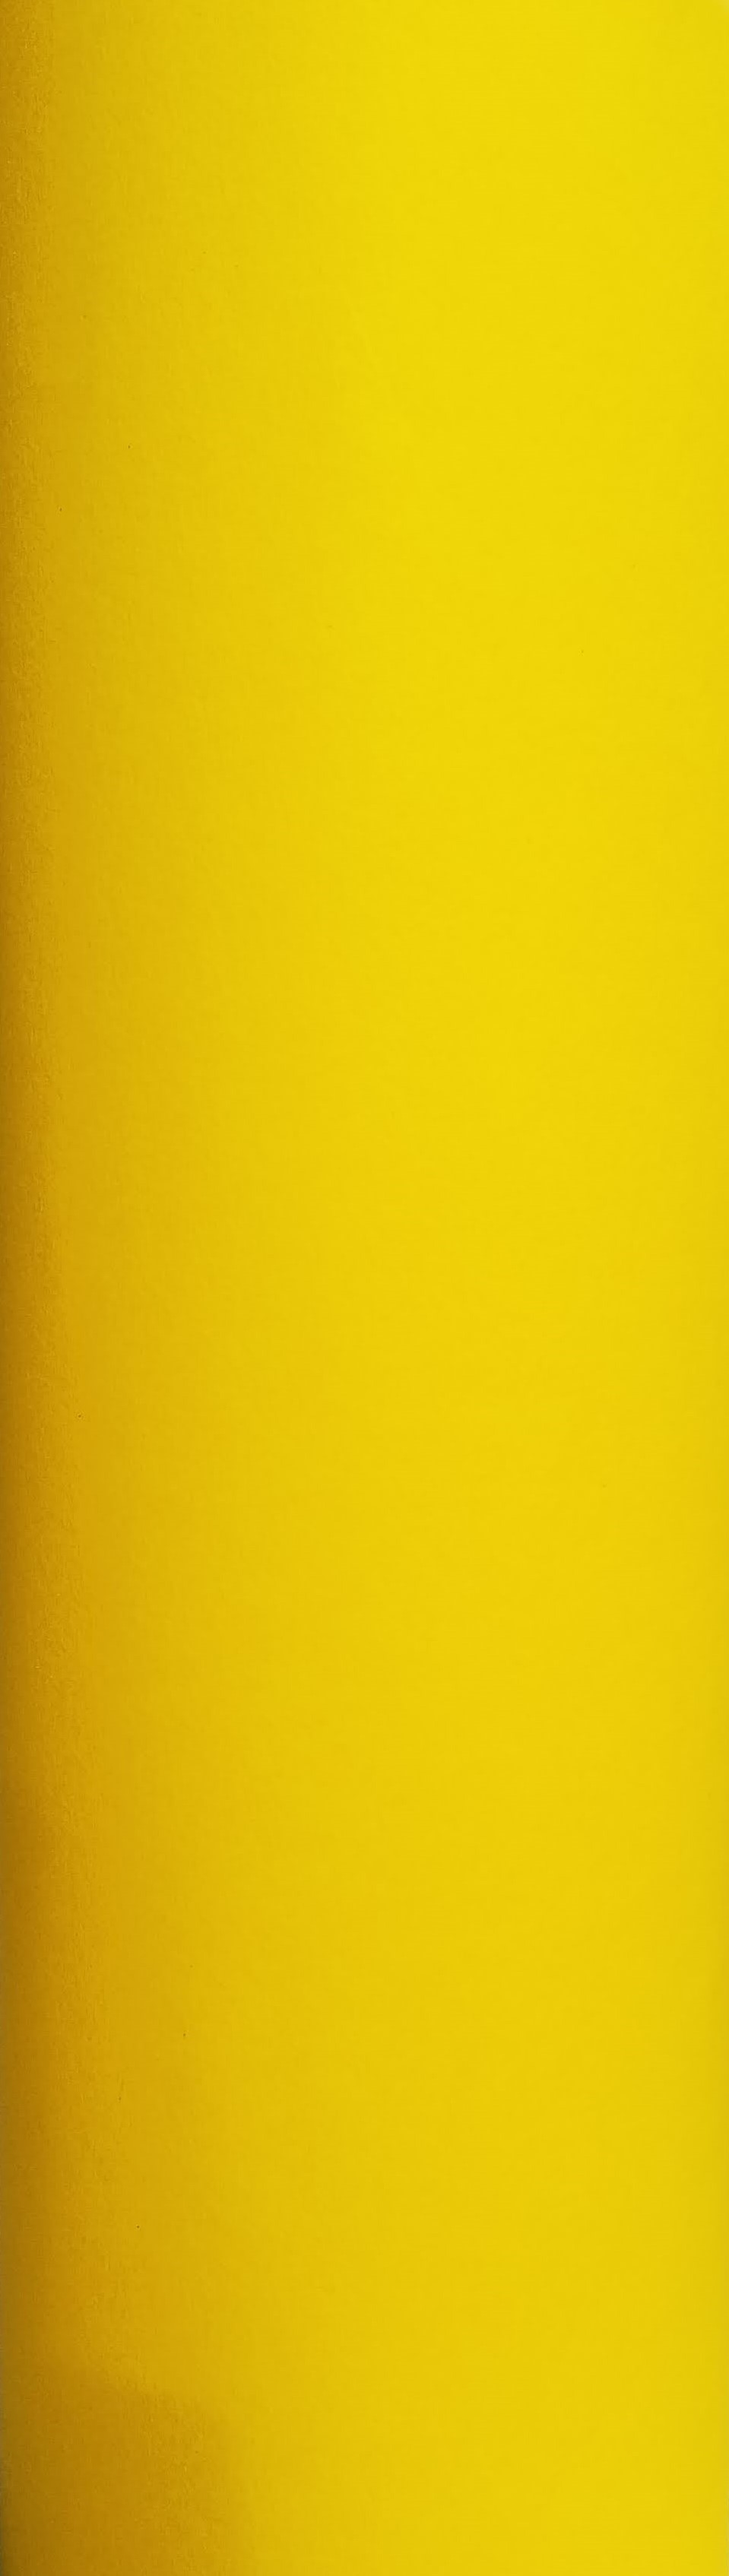
\includegraphics[width=.08\linewidth, height=.08\linewidth]{images/test_cut_03.jpg}
		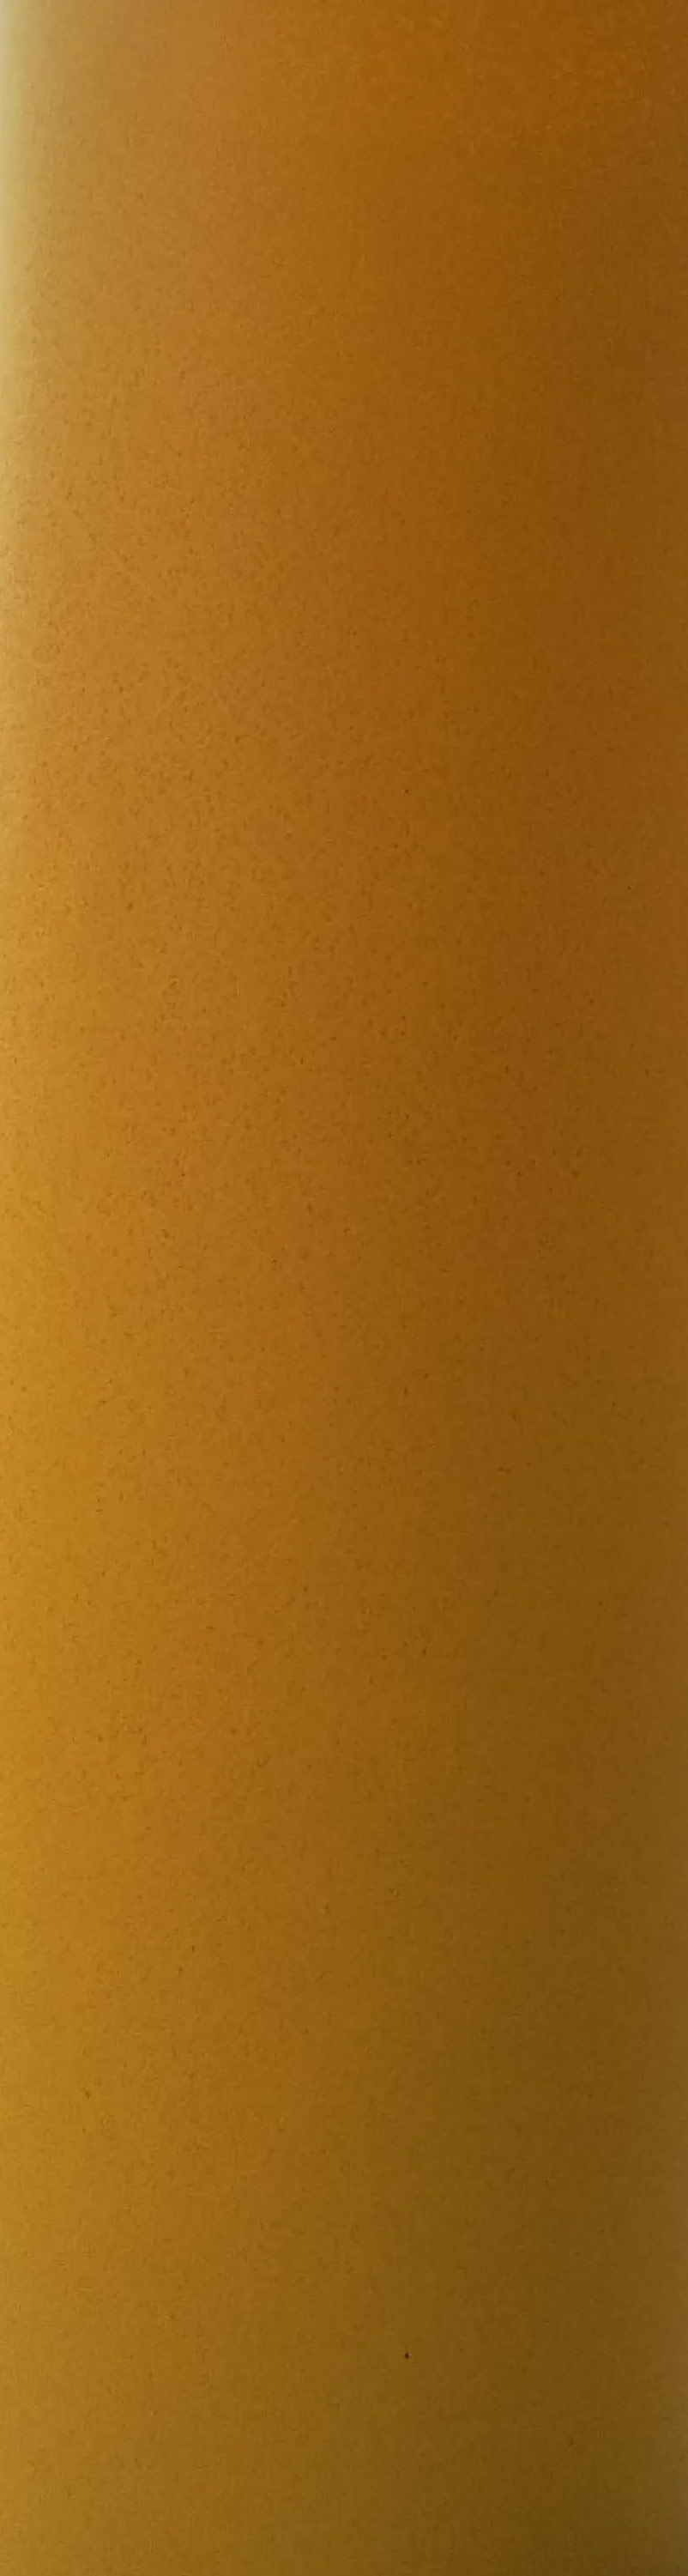
\includegraphics[width=.08\linewidth, height=.08\linewidth]{images/test_cut_04.jpg}
		
\includegraphics[width=.08\linewidth, height=.08\linewidth]{images/test_cut_05.jpg}
		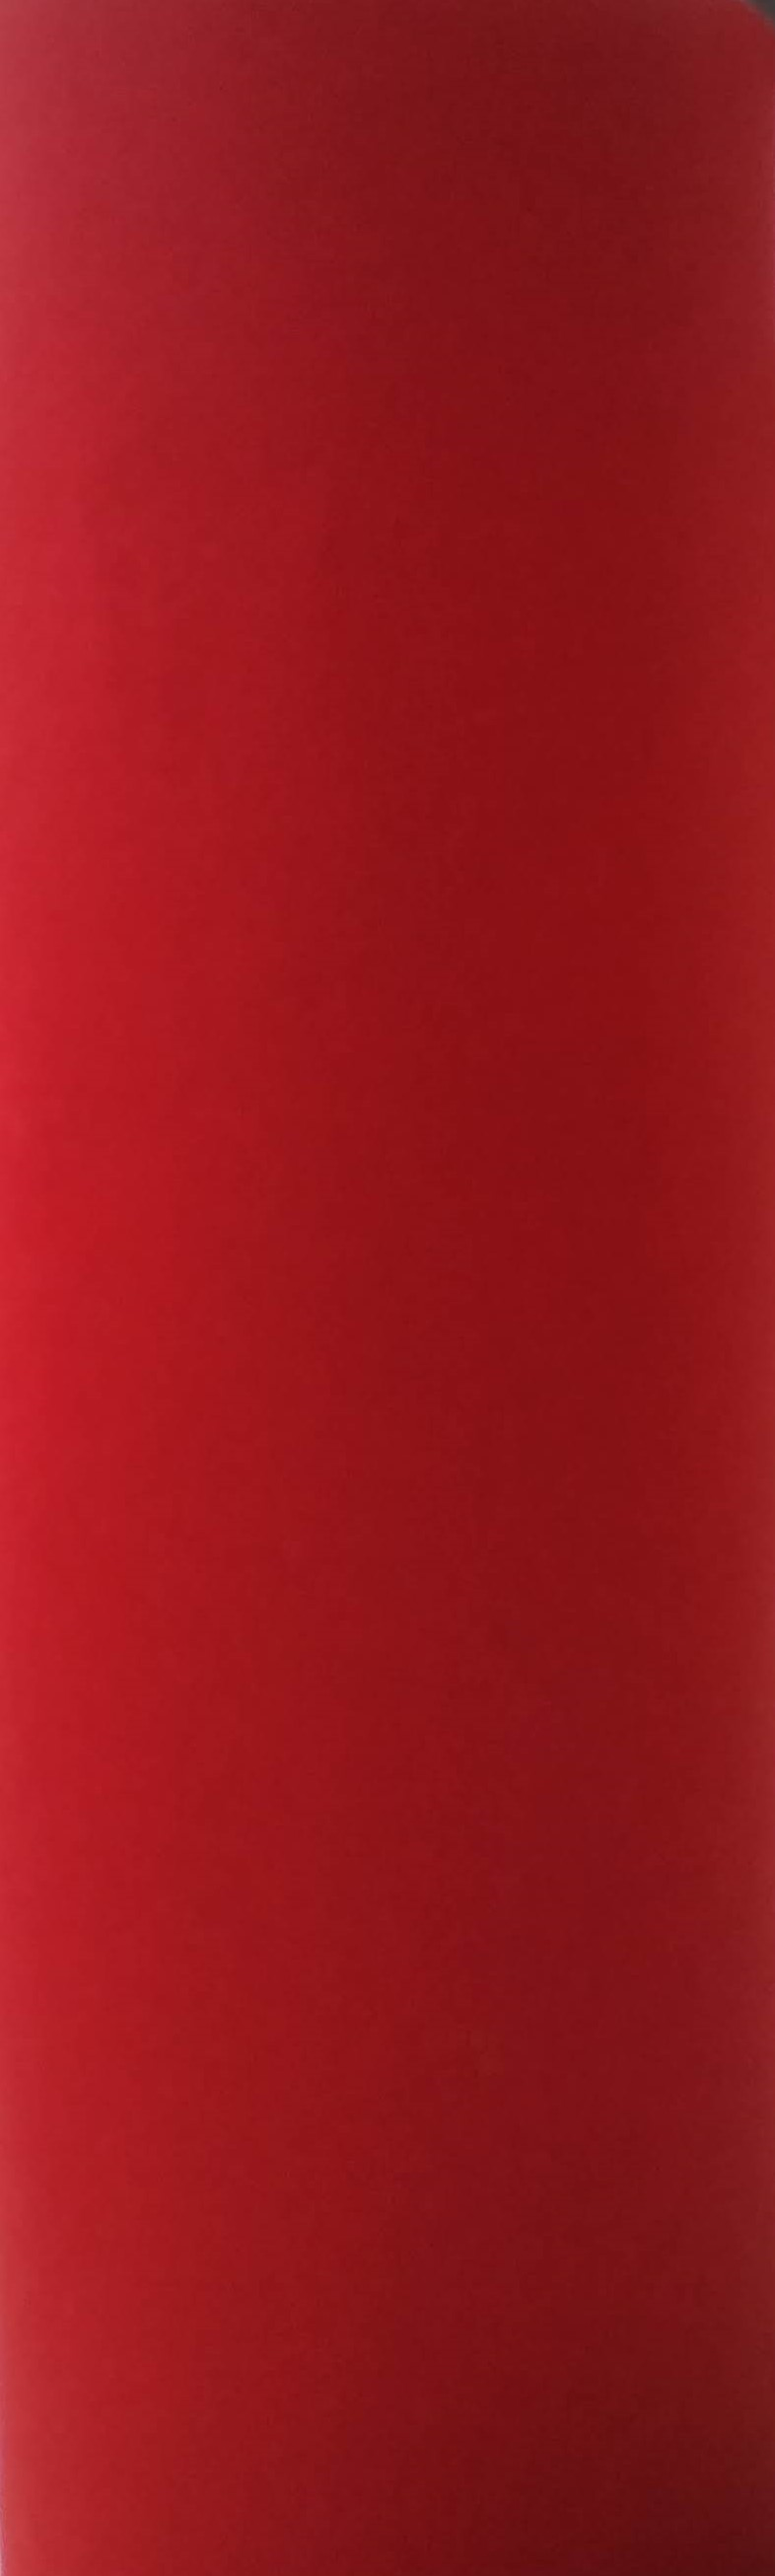
\includegraphics[width=.08\linewidth, height=.08\linewidth]{images/test_cut_06.jpg}
		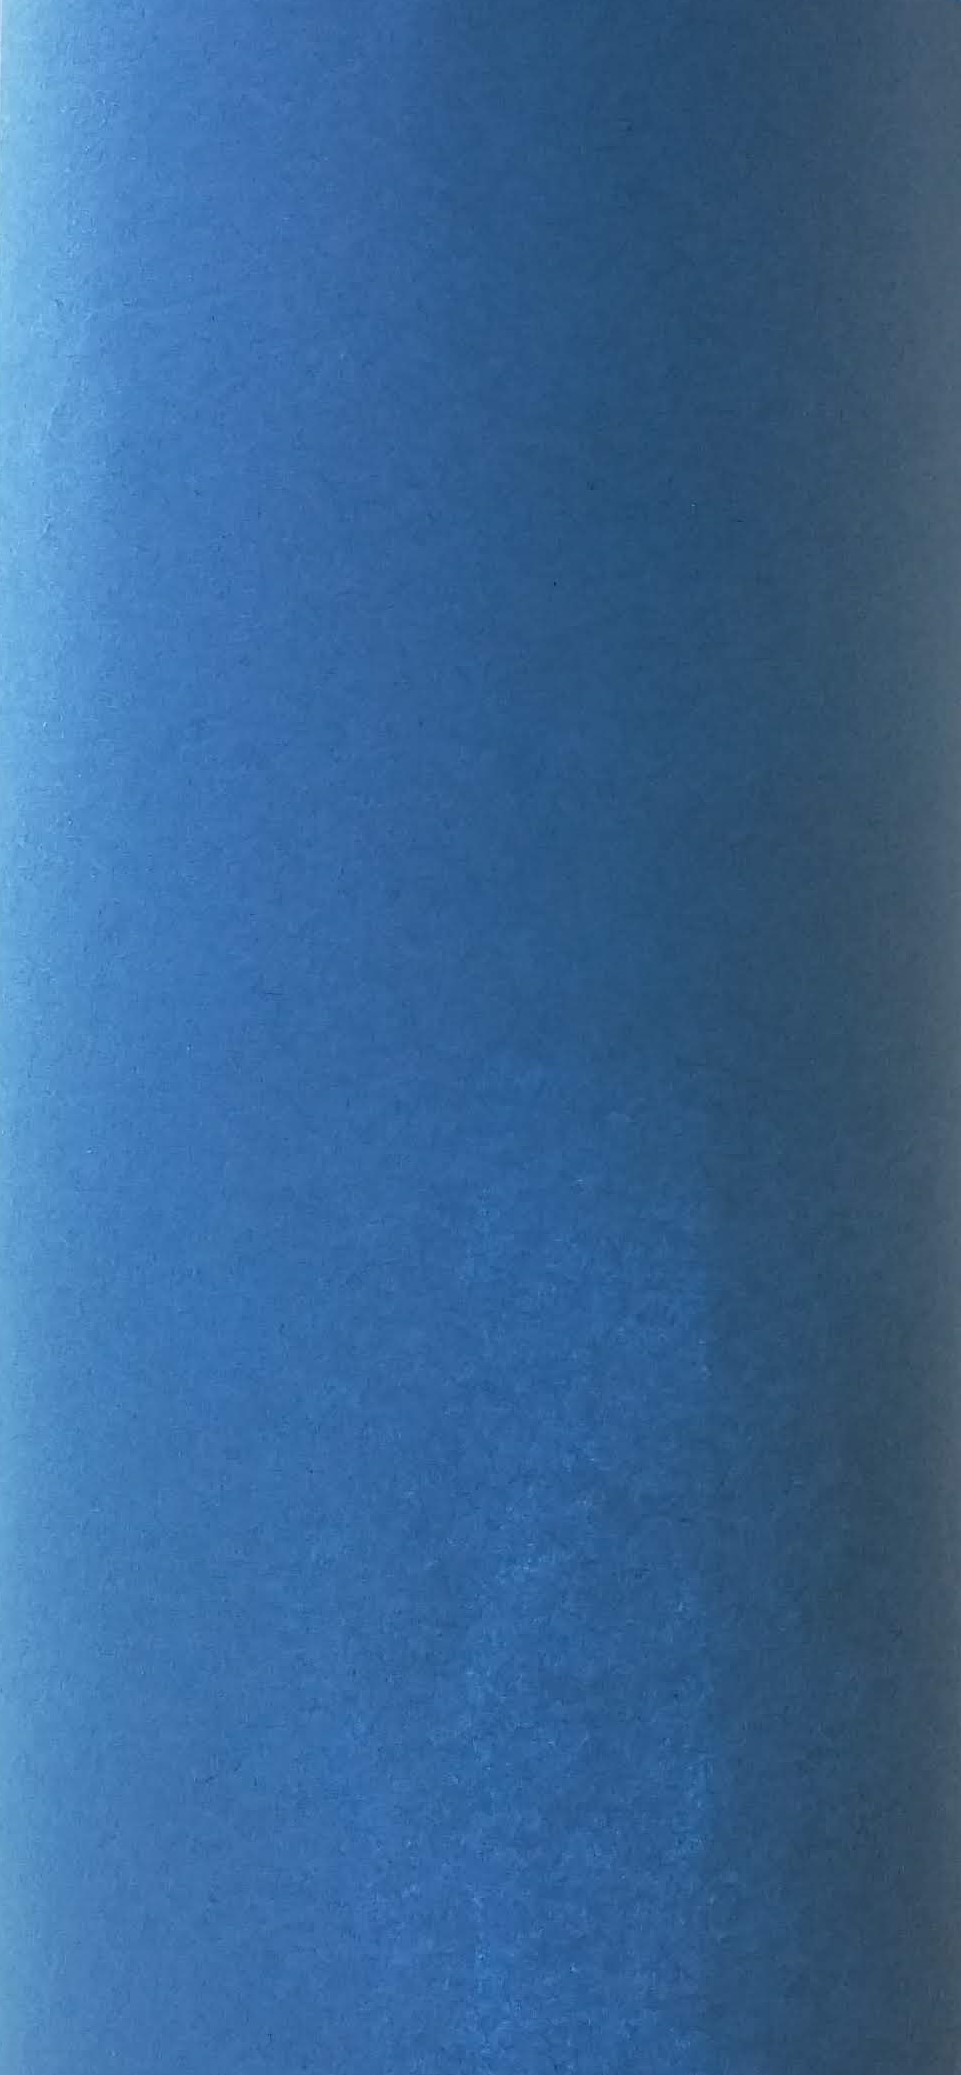
\includegraphics[width=.08\linewidth, height=.08\linewidth]{images/test_cut_07.jpg}
		
\includegraphics[width=.08\linewidth, height=.08\linewidth]{images/test_cut_08.jpg}
		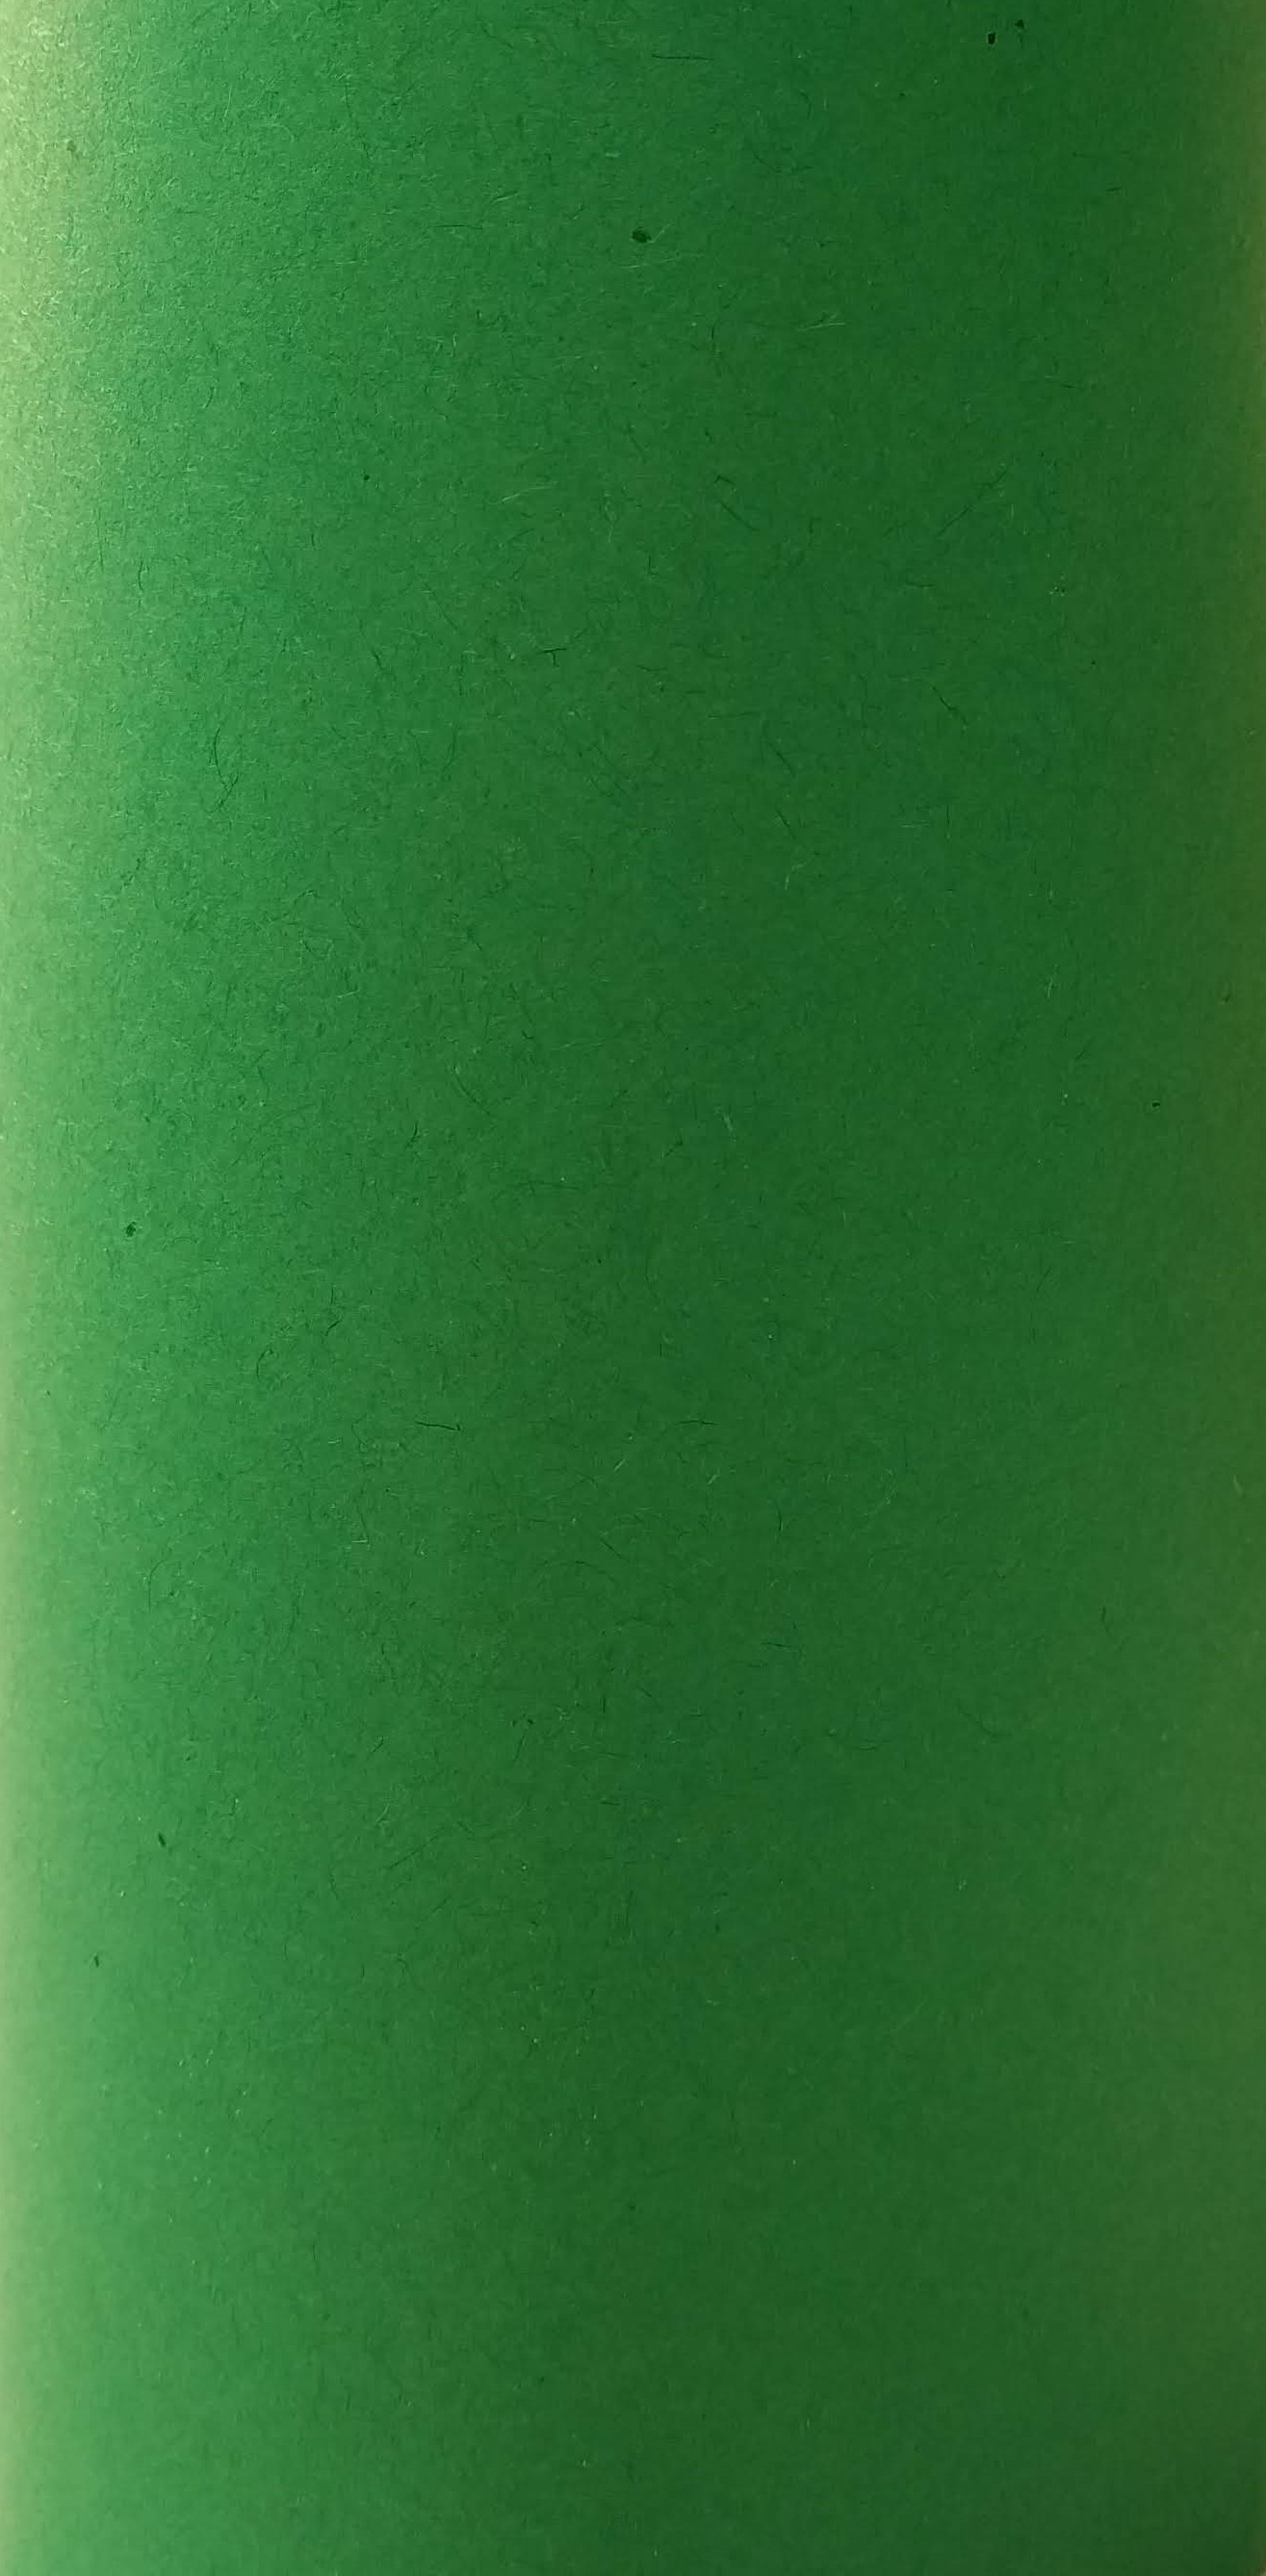
\includegraphics[width=.08\linewidth, height=.08\linewidth]{images/test_cut_09.jpg}
		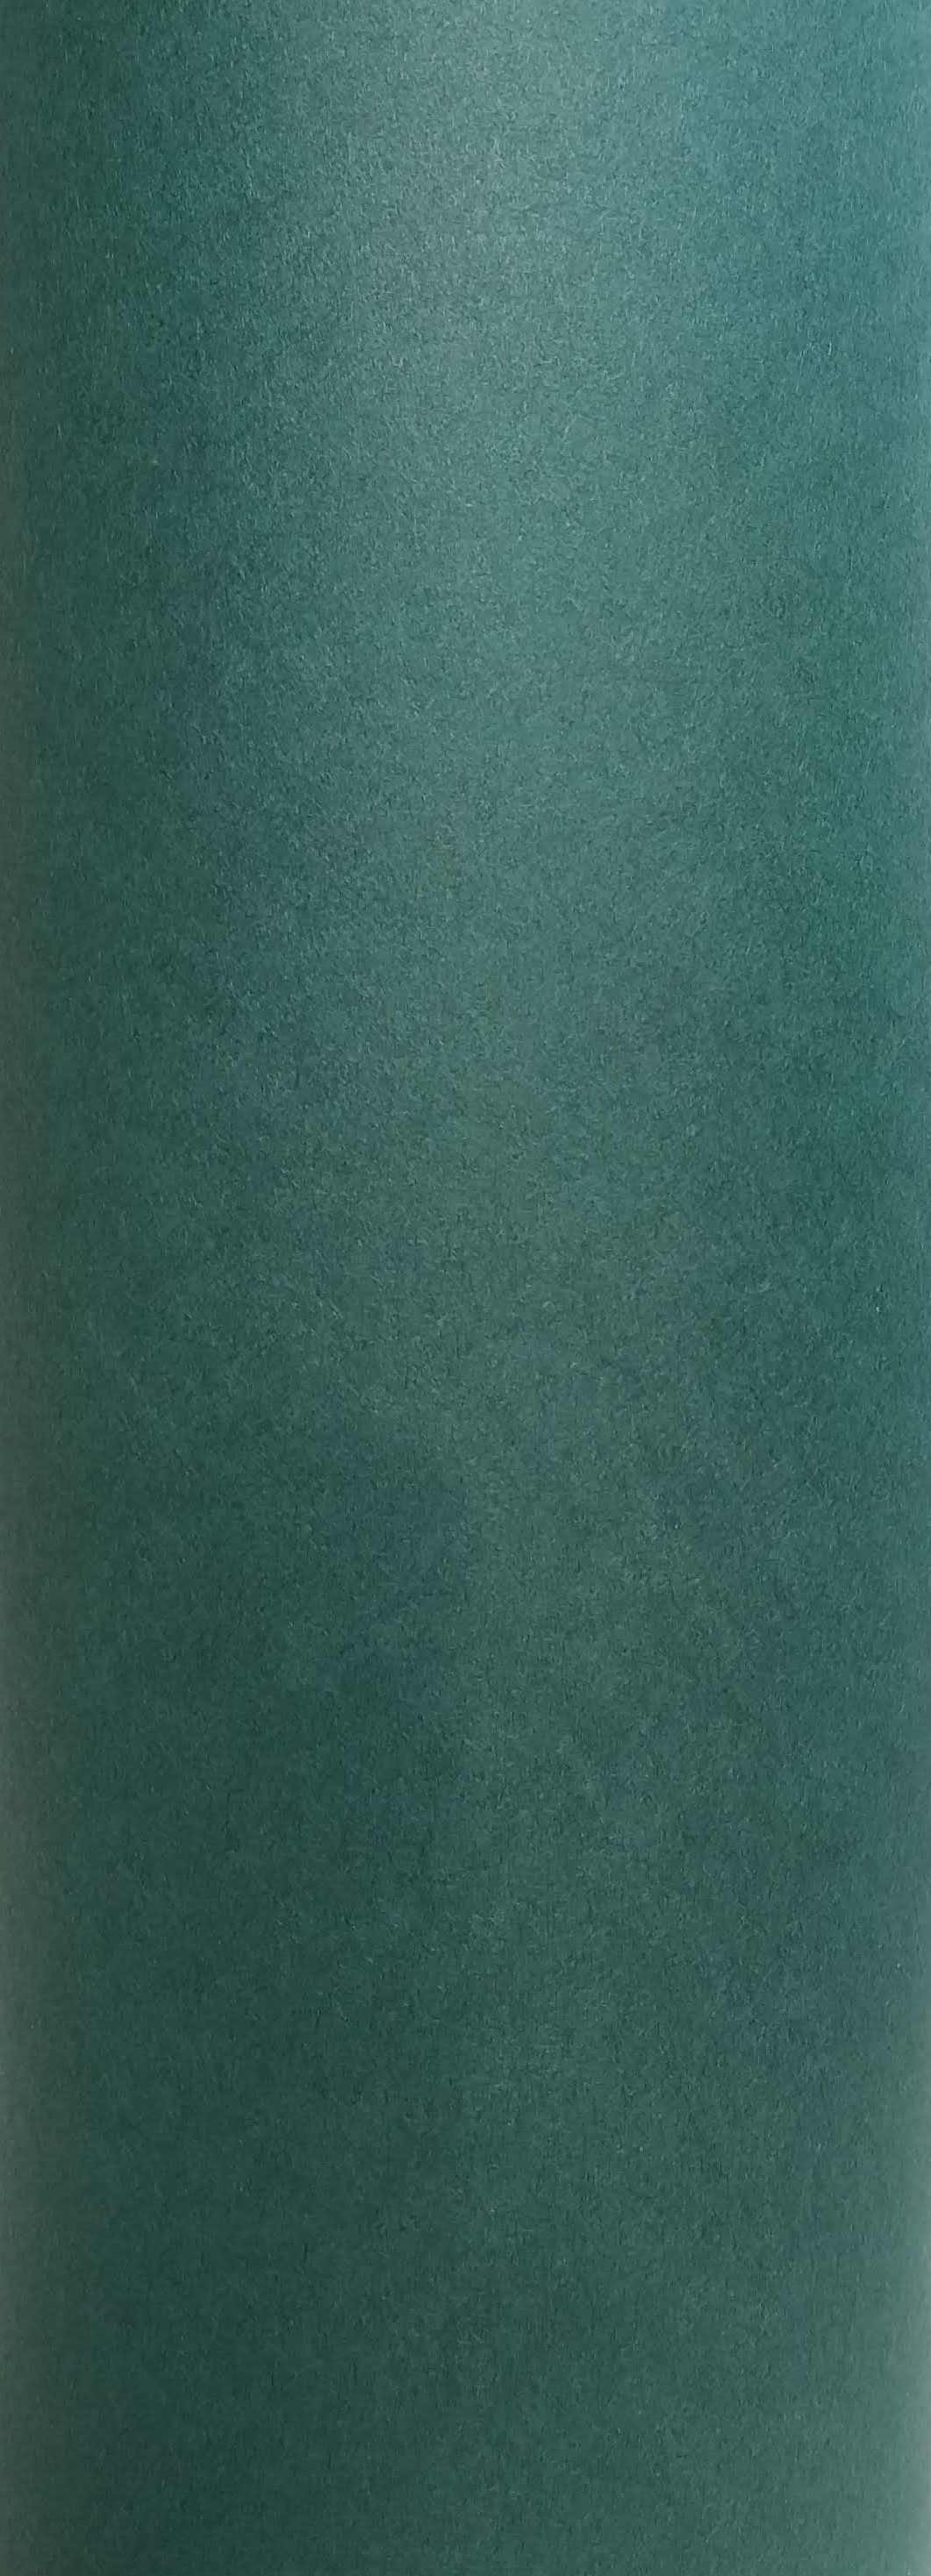
\includegraphics[width=.08\linewidth, height=.08\linewidth]{images/test_cut_10.jpg}
		
\includegraphics[width=.08\linewidth, height=.08\linewidth]{images/test_cut_11.jpg}
		\caption{Cropped images from second set}
	\end{figure}

	These cropped images illustrate very well, why we chose to use cylindrical objects as our test set. Each image contains various shades of the colour which is consequence of light hitting different spots on cylinders at different angle. Another reason for choosing this shape is that we expect encountering similar objects in the task2. 

	\subsection{Training and testing set}

	We split our data on training and testing set in a few different ways. First, we used the first set of images (circles) as our training set and the second set of images (cylinders) as our testing set. We expected this to be the best distribution, since the classifier can learn different shades of colours from the circles and then use that knowledge on images of clinders which have a few different shades of the same colour. \\

	For the second option we chose to swap the training and testing set to see if above hypotesis holds true.\\

	Since colour distribution is not the same among these two groups of images, we expected some missclassifications. The images of circles contain more dark tones as opposed to the images of cylinders.
	
	%TODO
	VSTAVI SLIKI BARVNIH DISTRIBUCIJ GLEDE NA MNOŽICO

	RAZMISLI ALI GRE TOLE ZDAJ RAJE V DISKUSIJO, ZAKAJ NI ACCURACY 1, ALI BOMO NARDILI ŠE TESTE ZA SET Z ENAKOMERNO RAZPOREDITVIJO
	We also noticed that the color within each set of images is not evenly distibuted. For example, the set of images of cylinders only contains 3 photos of black cylinders as opposed to XY photos of blue ones.
	
	\section{Colour classification}

	With our datasets ready, we then trained different classifiers to recognize colours and computed their accuracy on our testing set. To get the best classification accuracy, we also tried different colour spaces. 

	\subsection{Colour spaces}

	We tried \texttt{RGB}, \texttt{HSV} and \texttt{LAB} colourspace.\\

	Our first approach was training a classifier with colours as input vectors. Each colour in colour space can be represented by a vector $v$ and the classification task is to map this vector $v$ to correct class. \\
	
	In the \texttt{RGB} colour space, each vector $v$ can be represented using $v = (red, green, blue)$, where $red, green, blue \in [0, 255]$. \\

	Because the input to our classifier is a simple three dimensional vector, we predict that the knn classifier will perform quite well. \\	
	
	To prepare training data set, we used Hough transformation to detect circles in our images and randomly sampled points inside found circles to obtain RGB vectors corresponding to colours. Instead of sampling colour just from one point in the circle, we averaged colours in a region around sampled point. We chose multiple points from the same circle because object's illumination is almost never uniform. \\
	
	In the figure below we have plotted colours from our training set in \texttt{RGB} and \texttt{HSV} colour space. As we can see, in the \texttt{RGB} colour space, the shades of the same colour lie on the same line. Similar thing happens in \texttt{HSV} color space, but the lines are vertical. Because the \texttt{HSV} colour space is conical, the red colour lies both on the far left and far right of our graph. This is not ideal for knn or linear support vector machines, so we predict that those will perform better on the \texttt{RGB} colour space. \\
	
	The \texttt{RGB} and \texttt{HSV} are not natural colour spaces for humans. If two colours are close in \texttt{RGB} space (using euclidean distance), that doesn't mean that human perceive them as similar. There are some colour spaces that are more suited for human perception, for example the \texttt{CIELAB} colour space, also called \texttt{LAB}. \\

	\texttt{CIELAB} was designed so that the same amount of numerical change in these values corresponds to roughly the same amount of visually perceived change. The  \texttt{CIELAB} gamut includes both the gamuts of the \texttt{RGB} and \texttt{CYMK} color models. It expresses color as three values: $L^*$ for the lightness from black ($0$) to white ($100$), $a^*$ from green (−) to red ($+$), and $b^*$ from blue (−) to yellow ($+$). Because three parameters are measured, the space itself is a three-dimensional real number space, which allows for infinitely many possible colors. In practice, the space is usually mapped onto a three-dimensional integer space for digital representation, and thus the $L^*$, $a^*$, and $b^*$ values are usually absolute, with a pre-defined range. \\
	
	Since \texttt{LAB} is related to \texttt{RGB}, we can expect them to perform similarly.
	
	% ZAMENJAJ SLIKO KO DODAŠ ŠE BELO BARVO!
	\begin{center}
		\begin{figure}[H]
			\begin{subfigure}{.5\linewidth}
				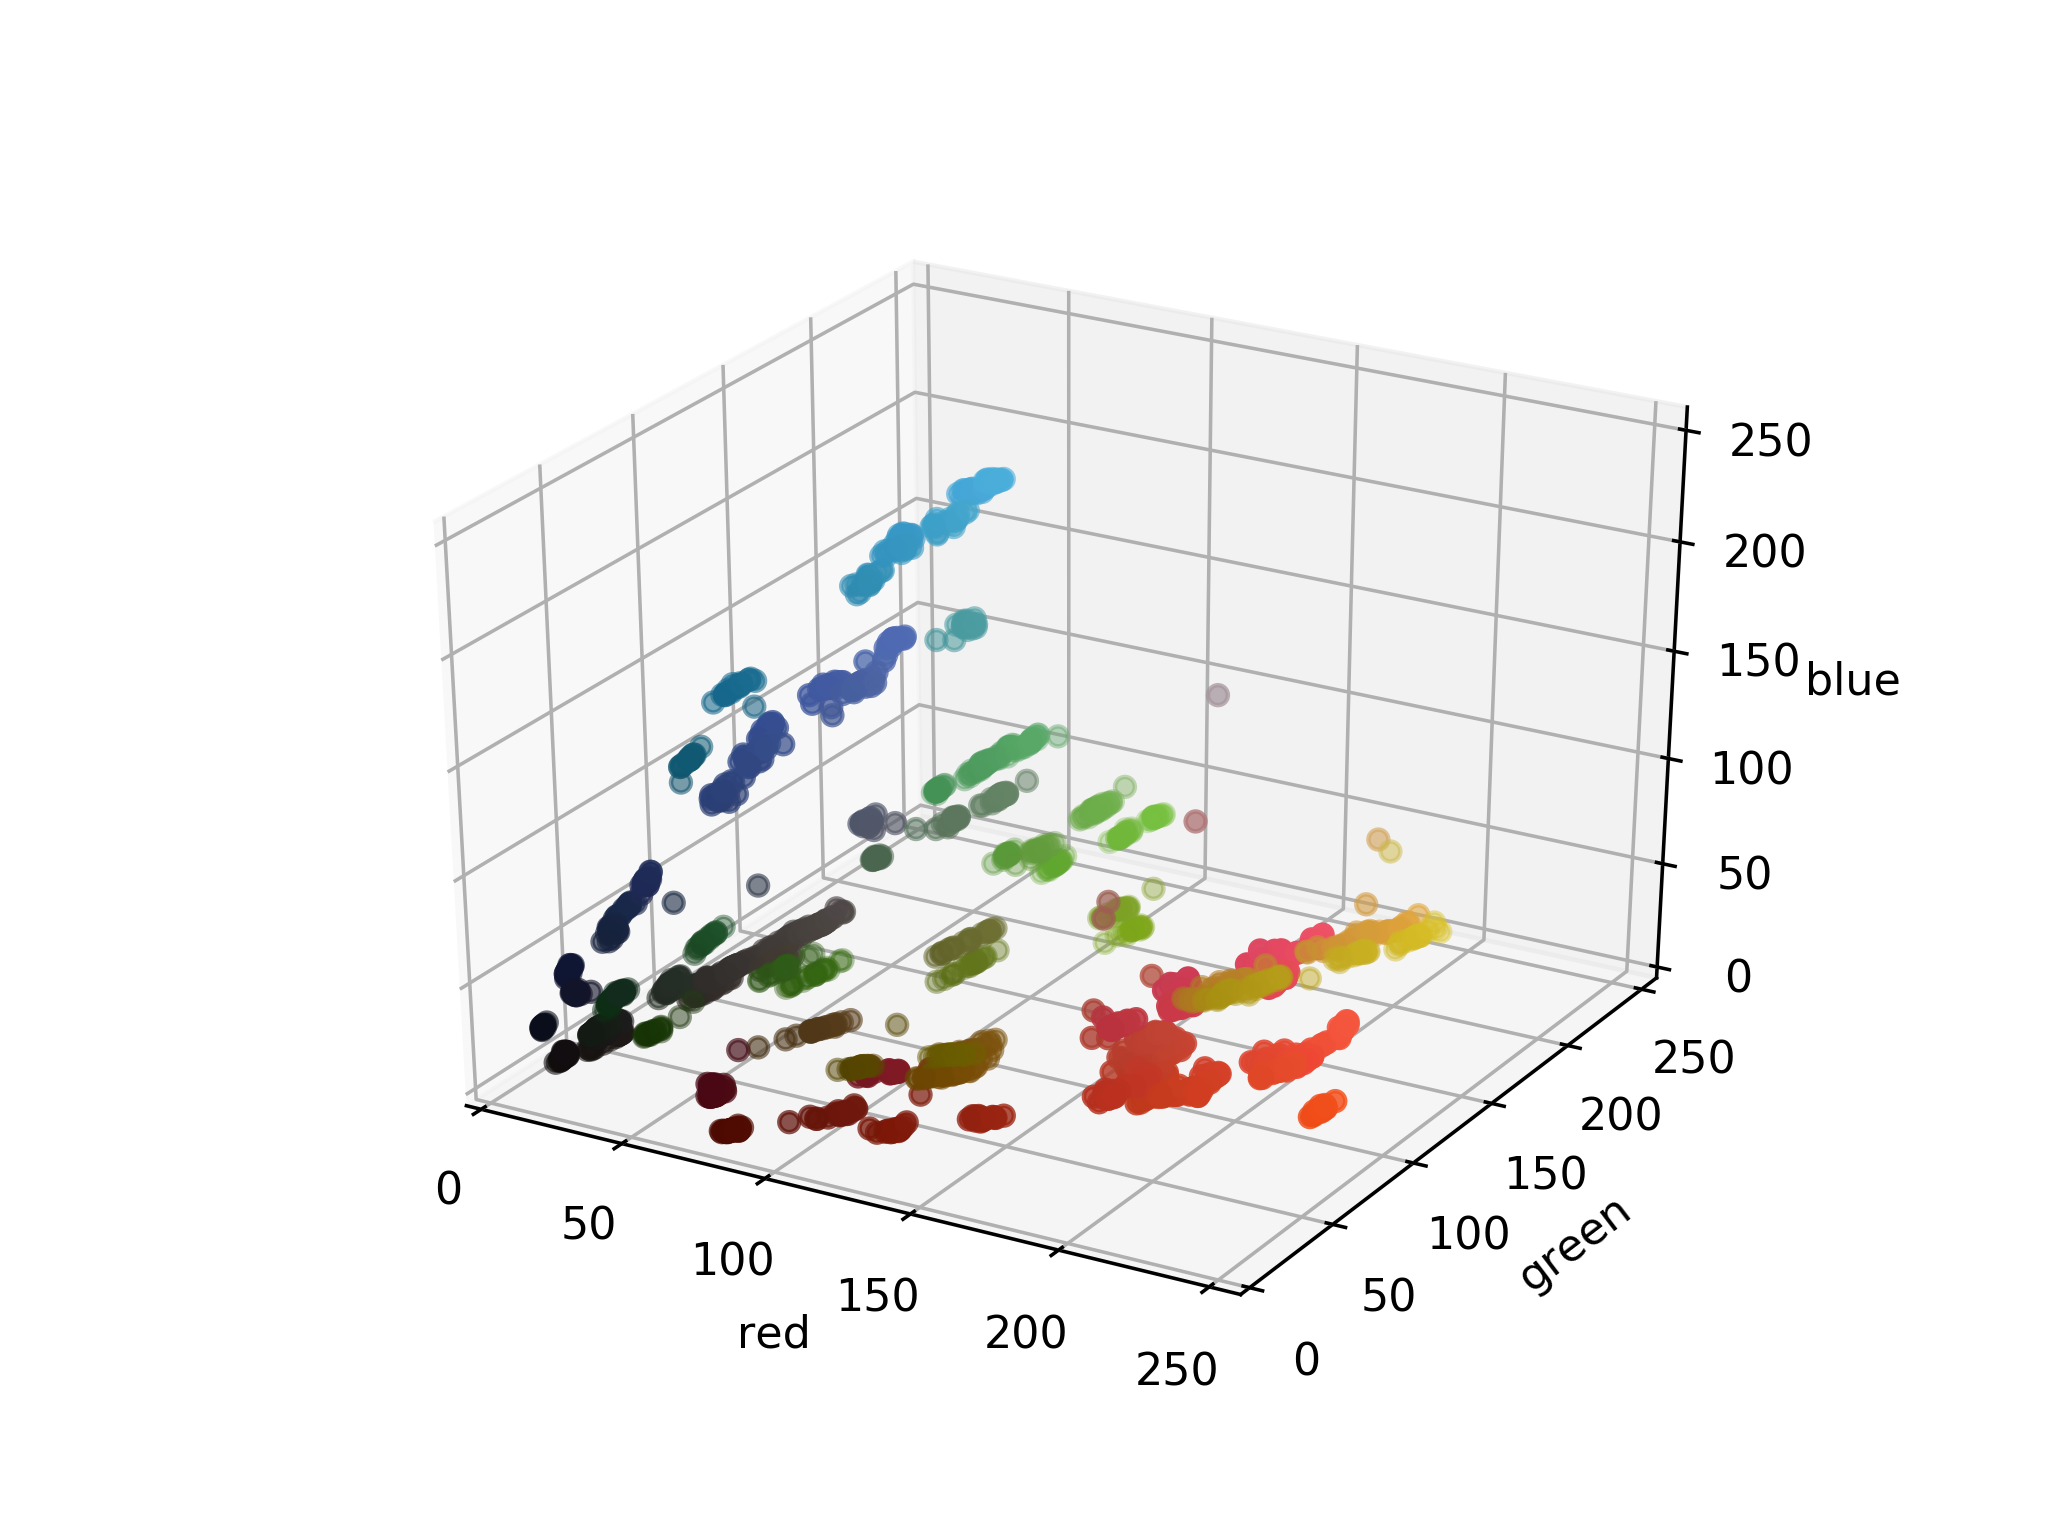
\includegraphics[width=\linewidth]{images/rgb.png}
				\caption{RGB color space}
			\end{subfigure}
			\begin{subfigure}{.5\linewidth}
				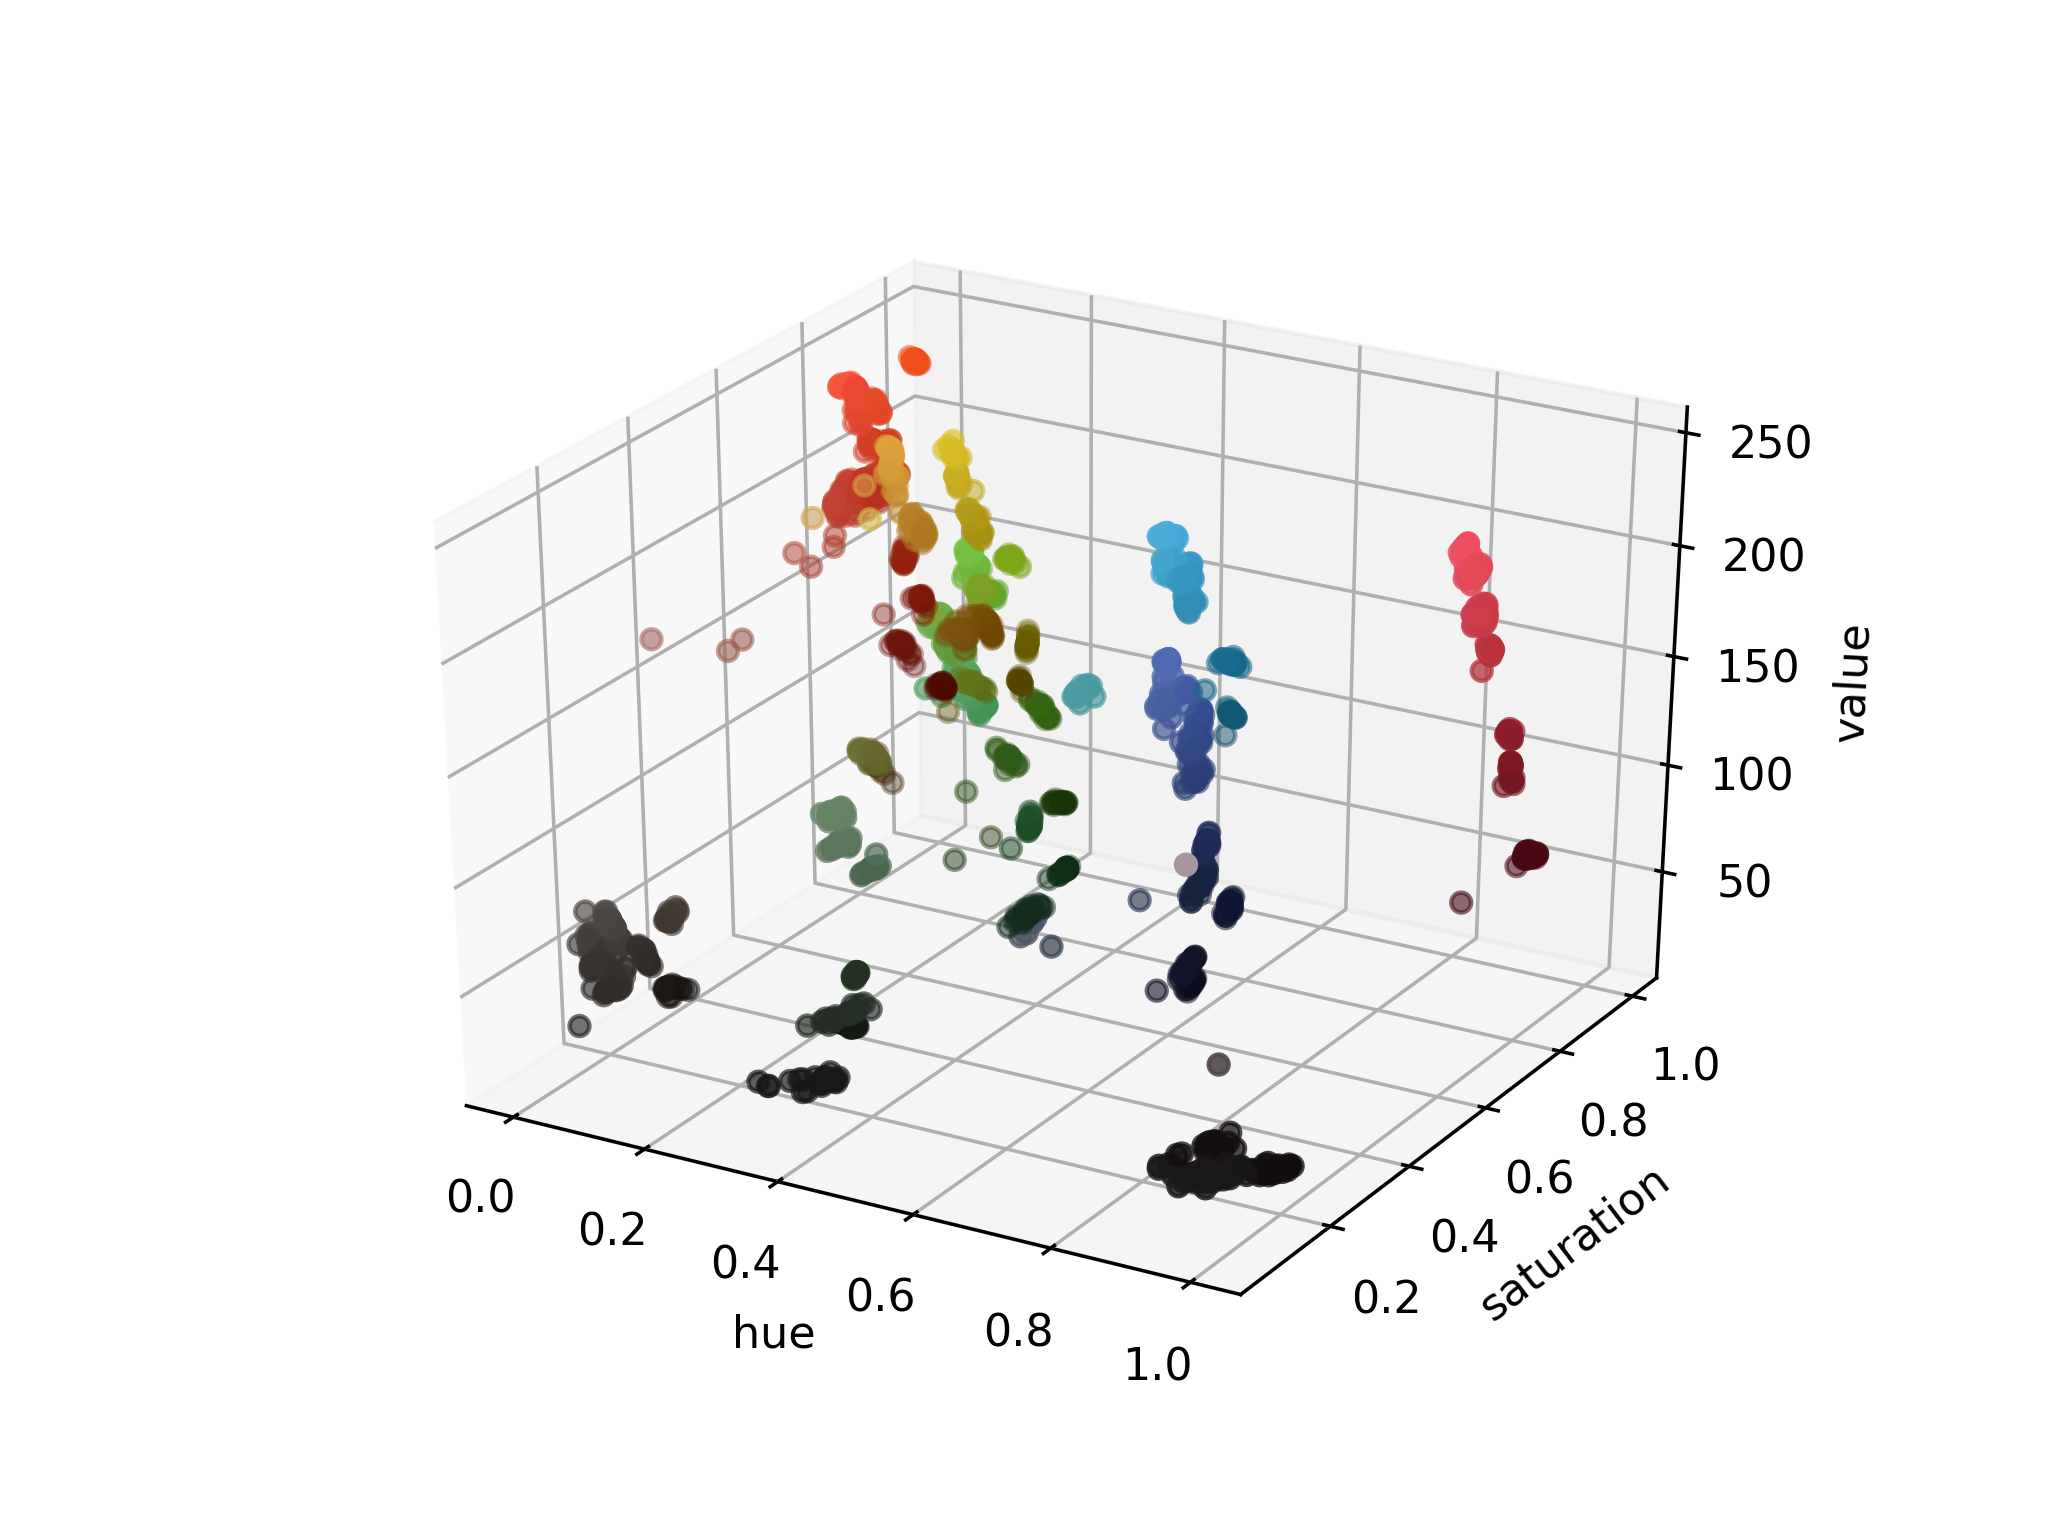
\includegraphics[width=\linewidth]{images/hsv.png}
				\caption{HSV color space}
			\end{subfigure}
		\end{figure}
	\end{center}

	\subsection{Colour distribution in training and testing set}

	MANJKA kk so razporejene barve, kaj smo nardili za enakomernost oziroma zakaj se za njo nismo odločli - A BO TU AL ZGORI
	% TODO: oštevilči vse opcije, ki smo jih sprobali

	\section{Evaluating performance}

	We then tested different classifiers using training data set. Results can be found in the table below. Accuracy is measured using our testing set and is calculated for all three coulour spaces \texttt{RGB}, \texttt{HSV} and \texttt{LAB} colour space.

	% A so že pravi podatki tu?
	
	\begin{center}
		\begin{tabular}{|c|c|c|c|}
			\hline 
			\textbf{Classifier} & \texttt{RGB} & \texttt{HSV} & \texttt{LAB} \\
			\hline
			knn, k = 1 & 0.88 & 0.52 & 0.94 \\ \hline
			knn, k = 1, weights = distance & 0.88 & 0.52 & 0.94 \\ \hline
			knn, k = 3 & 0.89 & 0.51 & 0.94 \\ \hline
			knn, k = 3, weights = distance & 0.89 & 0.52 & 0.94 \\ \hline
			knn, k = 5 & 0.89 & 0.53 & 0.94 \\ \hline
			knn, k = 5, weights = distance & 0.89 & 0.52 & 0.94 \\ \hline
			knn, k = 7 & 0.90 & 0.52 & 0.94 \\ \hline
			knn, k = 7, weights = distance & 0.90 & 0.53 & 0.94 \\ \hline
			decision tree, gini & 0.80 & 0.88 & 0.86 \\ \hline
			decision tree, entropy & 0.82 & 0.87 & 0.85 \\ \hline
			random forest, gini & 0.85 & 0.82 & 0.91 \\ \hline
			random forest, entropy & 0.82 & 0.85 & 0.89 \\ \hline
			naive bayes & 0.71 & 0.87 & 0.96 \\ \hline
			support vector machine, kernel=linear, c=0.025 & 0.92 & 0.61 & 0.92 \\ \hline
			support vector machine, kernel=rbf, c=0.025 & 0.26 & 0.42 & 0.27 \\ \hline
			support vector machine, kernel=linear, c=0.05 & 0.92 & 0.62 & 0.93 \\ \hline
			support vector machine, kernel=linear, c=0.1 & 0.92 & 0.50 & 0.93 \\ \hline
			support vector machine, kernel=linear, c=0.2 & 0.92 & 0.57 & 0.93 \\ \hline
		\end{tabular} \\
	\end{center}

	As we have predicted, the accuracy in \texttt{HSV} color space is lower than that in the \texttt{RGB} space. As expected, \texttt{RGB} and \texttt{LAB} perform similarly, but the \texttt{LAB} performs slightly better. \\
	
	% MANJKA IZBOR NAJBOLJŠEGA KLASIFIKATORJA
	
	% ZA VSAK KLASIFIKATOR NAPIŠI OPOMBO ZAKAJ JE TAKO

	
	\section{Conclusion}

	MANJKA kaj bomo uporabli na robotku, povzetek vsega, ovire (kot navedeno spodaj - dodaj osvetlitev)
	
	% OPOMBA GLEDE TEGA, DA JE POTREBNO IZ OBROČKA DOBITI PRAVO BARVO.
	As we can see from the table above, this type of classification works well. The only problem is that we have to choose points on our object, which can sometimes be problematic. But if we sample multiple points, the probability that our classification will be correct increases.
	
	
\end{document}